% !TeX spellcheck = en_GB
\documentclass{article}

% \usepackage[margin=1in,includefoot]{geometry}
\usepackage{graphicx}
\usepackage{titlesec}
\usepackage{array}
\usepackage[table]{xcolor}
\usepackage{color, colortbl}
\usepackage{stackengine}
\usepackage{fancyhdr}
\usepackage{longtable}
\usepackage{changepage}
\usepackage{tikz, graphicx}
\usepackage{hyperref}
\usepackage{listings}
\usepackage{alloy_language}
\usepackage{float}

\newcommand\xrowht[2][0]
{\addstackgap[.5\dimexpr#2\relax]{\vphantom{#1}}}
% \newcolumntype{C}{>{\centering\arraybackslash}p{0.6cm}}
% \newcolumntype{D}{>{\centering\arraybackslash}p{10cm}}
% \setlength{\parskip}{1em}

\setlength{\arrayrulewidth}{0.4mm}
\setlength{\tabcolsep}{20pt}
\renewcommand{\arraystretch}{1.6}
\setcounter{tocdepth}{4}
\setcounter{secnumdepth}{4}

\pagestyle{fancy}
\renewcommand{\headrulewidth}{2pt}
\renewcommand{\footrulewidth}{1pt}

\begin{document}
\begin{titlepage}
	\begin{center}
		\begin{figure}
			\centering
			
\includegraphics[scale=0.3]{LogoPolimi.PNG} \\
			[0.3cm]
		\end{figure}
		\Huge{\bfseries - RASD -} \\
		[0.5cm]
		\huge{Requirements Analysis and
			
			Specification Document} \\
		[1mm]
		\rule{300pt}{3pt} \\
		[1.0cm]
		\textsc{\Large Computer Science and Engineering} \\ 
		\textsc{\Huge Software Engineering II} \\
		\textsc{\Large A.A. 2020/2021} \\
		[1cm]
		\textsc{\LARGE Daniele Mammone - 10625264} \\
		\textsc{\LARGE Gianmarco Naro - 10610374} \\
		\textsc{\LARGE Massimo Parisi - 10583470} \\
	\end{center}
\end{titlepage}

\newpage
	
	\renewcommand\contentsname{Contents}
	\tableofcontents
	
\newpage

\section{Introduction}

	\subsection{Purpose}
	
	The main target of this document is to describe the {\bfseries Customer Line-Up} (\emph{CLup}) software through functional and non-functional requirement and is used as contractual basis between the customer and the developer. The structure of the document follows the one studied during lectures and aims to describe faithfully the software behaviour in all of its aspects.
	
	\emph{CLup} is a mobile service usable through app, made both for store managers and customers. It facilitates customers to book a visit to a store and to get a spot on the queue for entering a store and, on the other hand, helps store managers to observe the new strict rules due to \emph{Covid-19}.
	
	\subsection{Scope}
	
	The main purpose of \emph{CLup} is to facilitate customers to access at a store in {\bfseries security}, both allowing them to reserve a spot on the queue for entering the store through the app and to book a visit at the store at a determined time of a certain day, selected by the user. Thanks to this, store managers can manage the {\bfseries affluence} in their store more easier, and moreover can reduce the crowd in front of the store, that is one of the main purpose of the application. The main idea is that the system assigns a number to each customers' reservations (both queue spot and booking), and when a person's number is called, he can enter the supermarket. For this purpose, the app generates a \emph{QR Code} associated to the reservation, useful to check-in and check-out a customer in the store. Thanks to this, the system knows who is inside the store, and saves informations about customers' shopping sessions. By this data, it's possible to estimate time needed by people to complete what they need to do inside the store, and to calculate the \emph{ETA} to enter the store from a specific moment. Also, \emph{CLup} can suggest customers alternatives to their choose, either reserving a spot on the queue, and booking a visit. For customers without an electronic device, it's possible to get into the queue at a totem, installed at each store entry. Since someone may need to use only a part of the store, customers can select only the department of their interest; the aim of this is to decrease waiting times. At least, for reservation made by app, notifications are sent when someone must depart from his location, to get to store in time for his turn. The line up management must be {\bfseries fair}, to avoid regrettable situations such as can't entering to the store without booking or trying to access the store when it's the turn of somebody else. In the case the queue goes over the store working hours, customers are alerted by a warning message on their tickets.

	In the following sections, there are described {\bfseries World and Shared Phenomenons} through the "World and Machine" paradigm. In Shared Phenomena section, the \emph{M} stands for phenomenons controlled by Machine and observed by world, \emph{W} the vice versa.


		
		\subsubsection{World Phenomena}
		
		\bigskip
		
		\begin{center}
			
			\rowcolors{2}{}{gray!20}
			\rowcolors{1}{gray!20}{white}
			\renewcommand{\arraystretch}{2.5}
		
			\begin{adjustwidth}{-2.3cm}{}
			\begin{tabular}[h!]{|m{2.5em}|m{37em}|}
				
				\hline
				\xrowht{5pt}
				WP1 & A user enters a store  \\
				\xrowht{5pt}
				WP2 & A user waits in a lineup \\
				\xrowht{5pt}
				WP3 & A user exits the supermarket \\
				\xrowht{5pt}
				WP4 & A certain number of people is inside the supermarket \\
				\xrowht{5pt}
				WP5 & A certain number of people is at a specific department of the supermarket \\
				\xrowht{5pt}
				WP6 & The \emph{Covid-19} pandemic imposes some restrictions on crowds of people\\
				\hline
			\end{tabular}
			\end{adjustwidth}
		
		\end{center}
	
		\smallskip
		
		\subsubsection{Shared Phenomena}
		
		\bigskip
	 
		\begin{center}
			
			\rowcolors{2}{}{gray!20}
			\rowcolors{1}{gray!20}{white}
			\renewcommand{\arraystretch}{2.5}
			
			\begin{adjustwidth}{-2.3cm}{}
			\begin{tabular}[h!]{|m{2.5em}|m{32em}|m{1em}|}
				
				\hline
				\xrowht{5pt}
				SP1 & Customers get a spot on the queue & W\\
				\xrowht{5pt}
				SP2 & Customers book a visit to the store & W\\
				\xrowht{5pt}
				SP3 & Customers using app knows when they should depart for the store & M\\
				\xrowht{5pt}
				SP4 & Customers come to knows how much time they have to wait before entering & M\\
				\xrowht{5pt}
				\xrowht{5pt}
				SP5 & Customers scan the \emph{QR code} and enters in the supermarket & W\\
				\xrowht{5pt}
				SP6 & Customers scan the \emph{QR code} and exits from the supermarket & W\\
				\xrowht{5pt}
				SP7 & Customers can indicate the categories of items that he intend to buy & W\\
				\xrowht{5pt}
				SP8 & Customers are called to enter the store & M\\
				\hline
				
			\end{tabular}
			\end{adjustwidth}
		
		\end{center}
		
		\subsubsection{Goals}
		
		\bigskip
		
		\begin{center}
			
			\rowcolors{2}{}{gray!20}
			\rowcolors{1}{gray!20}{white}
			\renewcommand{\arraystretch}{2.5}
			
			\begin{adjustwidth}{-2.3cm}{}
			\begin{tabular}[h!]{|m{2.5em}|m{37em}|}
				
				\hline
				\xrowht{5pt}
				\centering G1 & Allow customers to select a store and book a visit on a certain date and time from \emph{CLup} app \\
				\xrowht{5pt}
				\centering G2 & Allow customers to select a store and take a spot on the queue to enter as soon as possible the store from \emph{CLup} app \\
				\xrowht{5pt}
				\centering G3 & Allow customers to book a spot on the queue from a physical ticket dispenser \\
				\xrowht{5pt}
				\centering G4 & Allow customers to have suggestions on better store options \\
				\xrowht{5pt}
				\centering G5 & Allow customers to decrease waiting times specifying departments they want to visit \\
				\xrowht{5pt}
				\centering G6 & Allow customers to manage their reservations \\
				\xrowht{5pt}
				\centering G7 & Allow customers to depart from their location in time to avoid waiting too much, and to avoid losing their turn for entering \\
				\xrowht{5pt}
				\centering G8 & Allow the store manager to know the real situation of people that are inside the building and in which departments of his store \\
				\xrowht{5pt}
				\centering G9 & Allow to grant a fair management of users that can access the building \\
				\xrowht{5pt}
				\centering G10 & Allow to manage optimally the influx in the building and avoid gathering inside it \\
				\xrowht{5pt}
				\centering G11 & Allow the store manager to interact with customers and their reservations \\
				\hline
				
				
			\end{tabular}
			\end{adjustwidth}
		\end{center}
	
		\bigskip
		
	\subsection{Definitions, Acronyms, Abbreviations}
	
		\smallskip
		
		\subsubsection{Definitions}
		
		\begin{center}
			
			\rowcolors{2}{}{gray!20}
			\rowcolors{1}{gray!20}{white}
			\renewcommand{\arraystretch}{2.5}
			
			\begin{adjustwidth}{-2.3cm}{}
			\begin{tabular}[h!]{|m{8em}|m{31em}|}
				
				
				\hline
				\xrowht{5pt}
				QR Code & Bi dimensional bar code that allows the user to check-in/check-out at the store entries/exits \\
				\xrowht{5pt}
				Reservation & Indicates both booked visits and spots on the queue to enter the store as soon as possible
				\\
				\xrowht{5pt}
				Customer & The clients of the store, that uses the system to get a reservation to access the store \\
				\xrowht{5pt}
				Store manager & The app user that access to stores' bookings, occupancy and settings, in order to manage the flow of customers \\
				\xrowht{5pt}
				QR Code Reader & Device used to scan customers' \emph{QR Code} \\
				\xrowht{5pt}
				Totem & Electronic device that allows customers to physically get a spot on the queue to enter the store as soon as possible; it allows to specify the same parameters that can be inserted through the app \\
				\xrowht{5pt}				
				QR Code Printer & Device used by totems to print \emph{QR Code} \\
				\xrowht{5pt}
				Department & Part of the store that contains the same category of products \\
				\hline
			\end{tabular}
			\end{adjustwidth}
			
		\end{center}
	
		\smallskip
		
		\subsubsection{Acronyms}
		
		\begin{center}
			
			\rowcolors{2}{}{gray!20}
			\rowcolors{1}{gray!20}{white}
			\renewcommand{\arraystretch}{2.5}
			
			\begin{adjustwidth}{-2.3cm}{}
			\begin{tabular}[h!]{|m{4em}|m{35em}|}
				
				\hline
				\xrowht{5pt}
				\centering RASD & Requirement Analysis and Specification Document \\
				\xrowht{5pt}
				\centering ETA & Estimated Time of Arrival \\
				\xrowht{5pt}
				\centering GPS & Global Positioning System \\
				\xrowht{5pt}
				\centering API & Application Programming Interface \\
				\xrowht{5pt}
				\centering UML & Unified Modeling Language \\
				\hline
				
			\end{tabular}
			\end{adjustwidth}
			
		\end{center}
	
		\bigskip
		
		\subsubsection{Abbreviations}
		
		\bigskip
		
		\begin{center}
			
			\rowcolors{2}{}{gray!20}
			\rowcolors{1}{gray!20}{white}
			\renewcommand{\arraystretch}{2.5}
			
			\begin{adjustwidth}{-2.3cm}{}
			\begin{tabular}[h!]{|m{2.5em}|m{36.5em}|}
				
				\hline
				\xrowht{5pt}
				WPn & World phenomena number n \\
				\xrowht{5pt}
				\centering SPn & Shared phenomena number n \\
				\xrowht{5pt}
				\centering Gn & Goal number n \\
				\xrowht{5pt}
				\centering Rn & Requirement number n \\
				\hline
				
			\end{tabular}
			\end{adjustwidth}
		\end{center}
	
		\smallskip
		
	\subsection{Revision History}
	
	\bigskip
	
	\begin{center}
		
		\renewcommand{\arraystretch}{1.5}
		\begin{adjustwidth}{-2.3cm}{}
		\begin{tabular}[h!]{|m{4em}|m{5em}|m{26em}|}
			
			\hline
			\rowcolor{gray!20}
			\xrowht{5pt}
			\centering Version & \centering Date & Changelog \\
			\hline
			\xrowht{5pt}
			\centering 1.0 & 29/11/2020 & First version \\
			\hline
			\xrowht{5pt}
			\centering 1.1 & 05/12/2020 & Update of some domain assumption and functional requirements \\
			\hline
			\xrowht{5pt}
			\centering 1.2 & 17/12/2020 & Update of some use cases and other fixes in order to be consistent with queue management \\
			\hline
			\xrowht{5pt}
			\centering 1.3 & 18/12/2020 & First revision \\
			\hline
			\xrowht{5pt}
			\centering 2.0 & 19/12/2020 & Stylistic revision of the document \\
			\hline
			\xrowht{5pt}
			\centering 2.1 & 23/12/2020 & Deliverable version\\
			\hline
			
		\end{tabular}
		\end{adjustwidth}
		
	\end{center}

	\bigskip
	
	\subsection{Software and Tools}
	
		\begin{itemize}
			\item {\LaTeX} as software system for docuement preparation
			\item Alloy as model analyzer
			\item UMLet for the UML diagrams and other diagrams
			\item Photoshop for the mockups
			\item Git \& Github as work space. The repository is \href{https://github.com/danmaam/MammoneNaroParisi}{here}.
		\end{itemize}
	
	\newpage
	
	\subsection{Reference Documents}
	
	\smallskip
	
	\begin{itemize}
		
		\item Specification Document
		\item Slides of the lectures
		
	\end{itemize} 
	
	\subsection{Document Structure}
	
	The structure of the document is thought with the intention of allowing simple navigation through it. Also, various abbreviations, highlighted in Abbreviations section, have been used to make the content smoother.
	Hence, the structure of the document is the following one:
	
	\begin{itemize}
		
		\item {\bfseries Introduction}: introduces in a general way the scope of the application through the analysis of the \emph{World Phenomena}, \emph{Shared Phenomena} and \emph{Goals}. Moreover, the main functions of the software are illustrated and the abbreviations, acronyms and definitions are reported in order to allow an easy reading.
		
		\item {\bfseries Overall Description}: The section starts with a summary description of the \emph{UML} of the software, so as to have a general presentation of the operations of the application. Then, in order to clarify the behavior of the system, there are state charts of the most important and critical functions and the detailed description of all software functions. Subsequently, the section ends with the most important phenomena that cannot be managed by the system.
		
		\item {\bfseries Specific Requirements}: The main focus of this section is to describe the essential hardware and software interfaces and requirements necessary to \emph{CLup} for providing its services. After this, there is the core of the section containing the use cases that provides detailed information about the interaction with the system.
		
		\item {\bfseries Formal Analysis Using Alloy}: This section describes formally the model using Alloy language, highlighting the main problems of the software, solving them in a formal way.
		
		\item {\bfseries Effort Spent}: The main focus of this section is to track the time spent to complete this project. In particular, is highlighted the subdivision of the working hours of the various sections
		
		\item {\bfseries References}: This section is dedicated to all references used in this project.
		
	\end{itemize}
	
\newpage	

\section{Overall Description}

	\subsection{Product Perspective}
	
	
	In \emph{Figure 1} is reported an {\bfseries UML Class Diagram} that represents the domain of the application with main concepts and data involved, including their relationships.
	
	The store managers registers to the application providing all the necessary informations and can decide at a later stage to modify some options (also regarding each department of the store), such as working hours for each week's day, capacities ecc. Customers download the application on their device and registers to the service to be able to use it, or requests ticket at the store entry. Here we can identify the main aspects related to \emph{CLup}:
	
	\begin{itemize}
		
		\item The customer can generate a {\bfseries reservation}, choosing between a registered chain store (and one of their specific store) or a normal store and, optionally, the departments that they want to access; \emph{CLup} will store the reservation and send customers a (digital) ticket containing the reservation's \emph{ID} and a \emph{QR Code}. Furthermore, the ticket contains the \emph{ETA} to enter the store, and it's always recalculated when it's visualized on the application.
		
		\item The customer can {\bfseries entry} in the store where he has a reservation (when his ticket's number is called to entry) scanning the \emph{QR Code} through the \emph{QR Code Reader}. The system registers his entry.
		
		\item The customer {\bfseries exits} the store reusing the same \emph{QR Code}, updating the number of people inside the store.
		
	\end{itemize}

	The \emph{UML} does not include every class of the actual implementation of the system.
		
		\subsubsection{UML Description}
		
			The {\bfseries UML Class Diagram} in \emph{Figure 1} contains many classes and in this section we are going to explain shortly their functions and their scope in the project.
			
			\begin{itemize}
				\item {\bfseries Transportation}: Is an abstract class that defines the generic means of transport that could be chosen by the customer, such as:
				
					\begin{itemize}
						\itemsep-0.20em
						\item Public transport
						\item On foot
						\item Bike
						\item Car
					\end{itemize}
				
				\item {\bfseries User}: Is an abstract class that defines the generic user that can use the application. An user could be either a customer or a store manager based on their privileges in the application.
				
					\begin{itemize}
						\item {\bfseries Customer}: Can generate a reservation and manage his ones. Moreover, each client is associated with his preferred mean of transport.						
						\item {\bfseries Store manager}: A store manager is associated to a store, and can manage it, modifying its parameters and working hours.
					\end{itemize}
				
				\item {\bfseries Statistic}: Is an abstract class that defines the generic statistic that can be used from the software to infer the customers' shopping time.			
				\begin{itemize}
					\item {\bfseries Customer statistics}: The system uses the customer statistic in order to provide the average time spent during a visit in the store by a specific user. If the customer, during a booking, decides to not specify the time that will be used during his shopping, the system make an estimation based on his previous visits.
					
					\item {\bfseries Department statistics}: The system uses the statistic obtained from customers that visit a certain department's store in order to calculate the average time spent by customers in each store's department. Having done this, if a customer does not have his personal statistic and decide to not specify the time that he will use during his shopping, the system can base its estimation on statistics of other customers. 
				
				\end{itemize}
			
				\item {\bfseries Store}: Represents the store with his unique \emph{ID}. Each store is related to its departments, increasing its granularity, so that store manager that can control its parameters in a detailed way, and so that customers can choose to visit only a part of it. Each store is associated with its map position, necessary to generate suggestions, and to know how much a customer need to reach the store's position from his location. Moreover, the store has a  queue of callable tickets, reservations for other days and the working hours for each day of the week, associated with a flag about store opening in that day.
				
				\item {\bfseries Department}: This class represents a store's department and is related to its statistics The store manager can modify the \emph{maxCapacity} and the \emph{maxAllowedBooking} parameters for each department's store in order to avoid an overcrowding inside the store, and to grant fair balance between allowed booked clients and non booked ones. Moreover, the class takes trace of each customer inside the specific store zone.
				
				\item {\bfseries Chain Store}: Each store can belongs to a chain
				
				\item {\bfseries Reservation}: Each reservation is associated to a customer and is managed by the store and it has many attributes that provides informations about both the entry and exit time (expected and effective).
				
				\item {\bfseries Ticket}: Every reservation has a ticket that provides the most important things: \emph{QR Code} and number to be called. Indeed, if a customer want enter or exit the shop, must scan his \emph{QR Code}.
			\end{itemize}
		
		\begin{figure}
			\begin{adjustwidth}{-3cm}{}
				\centering
				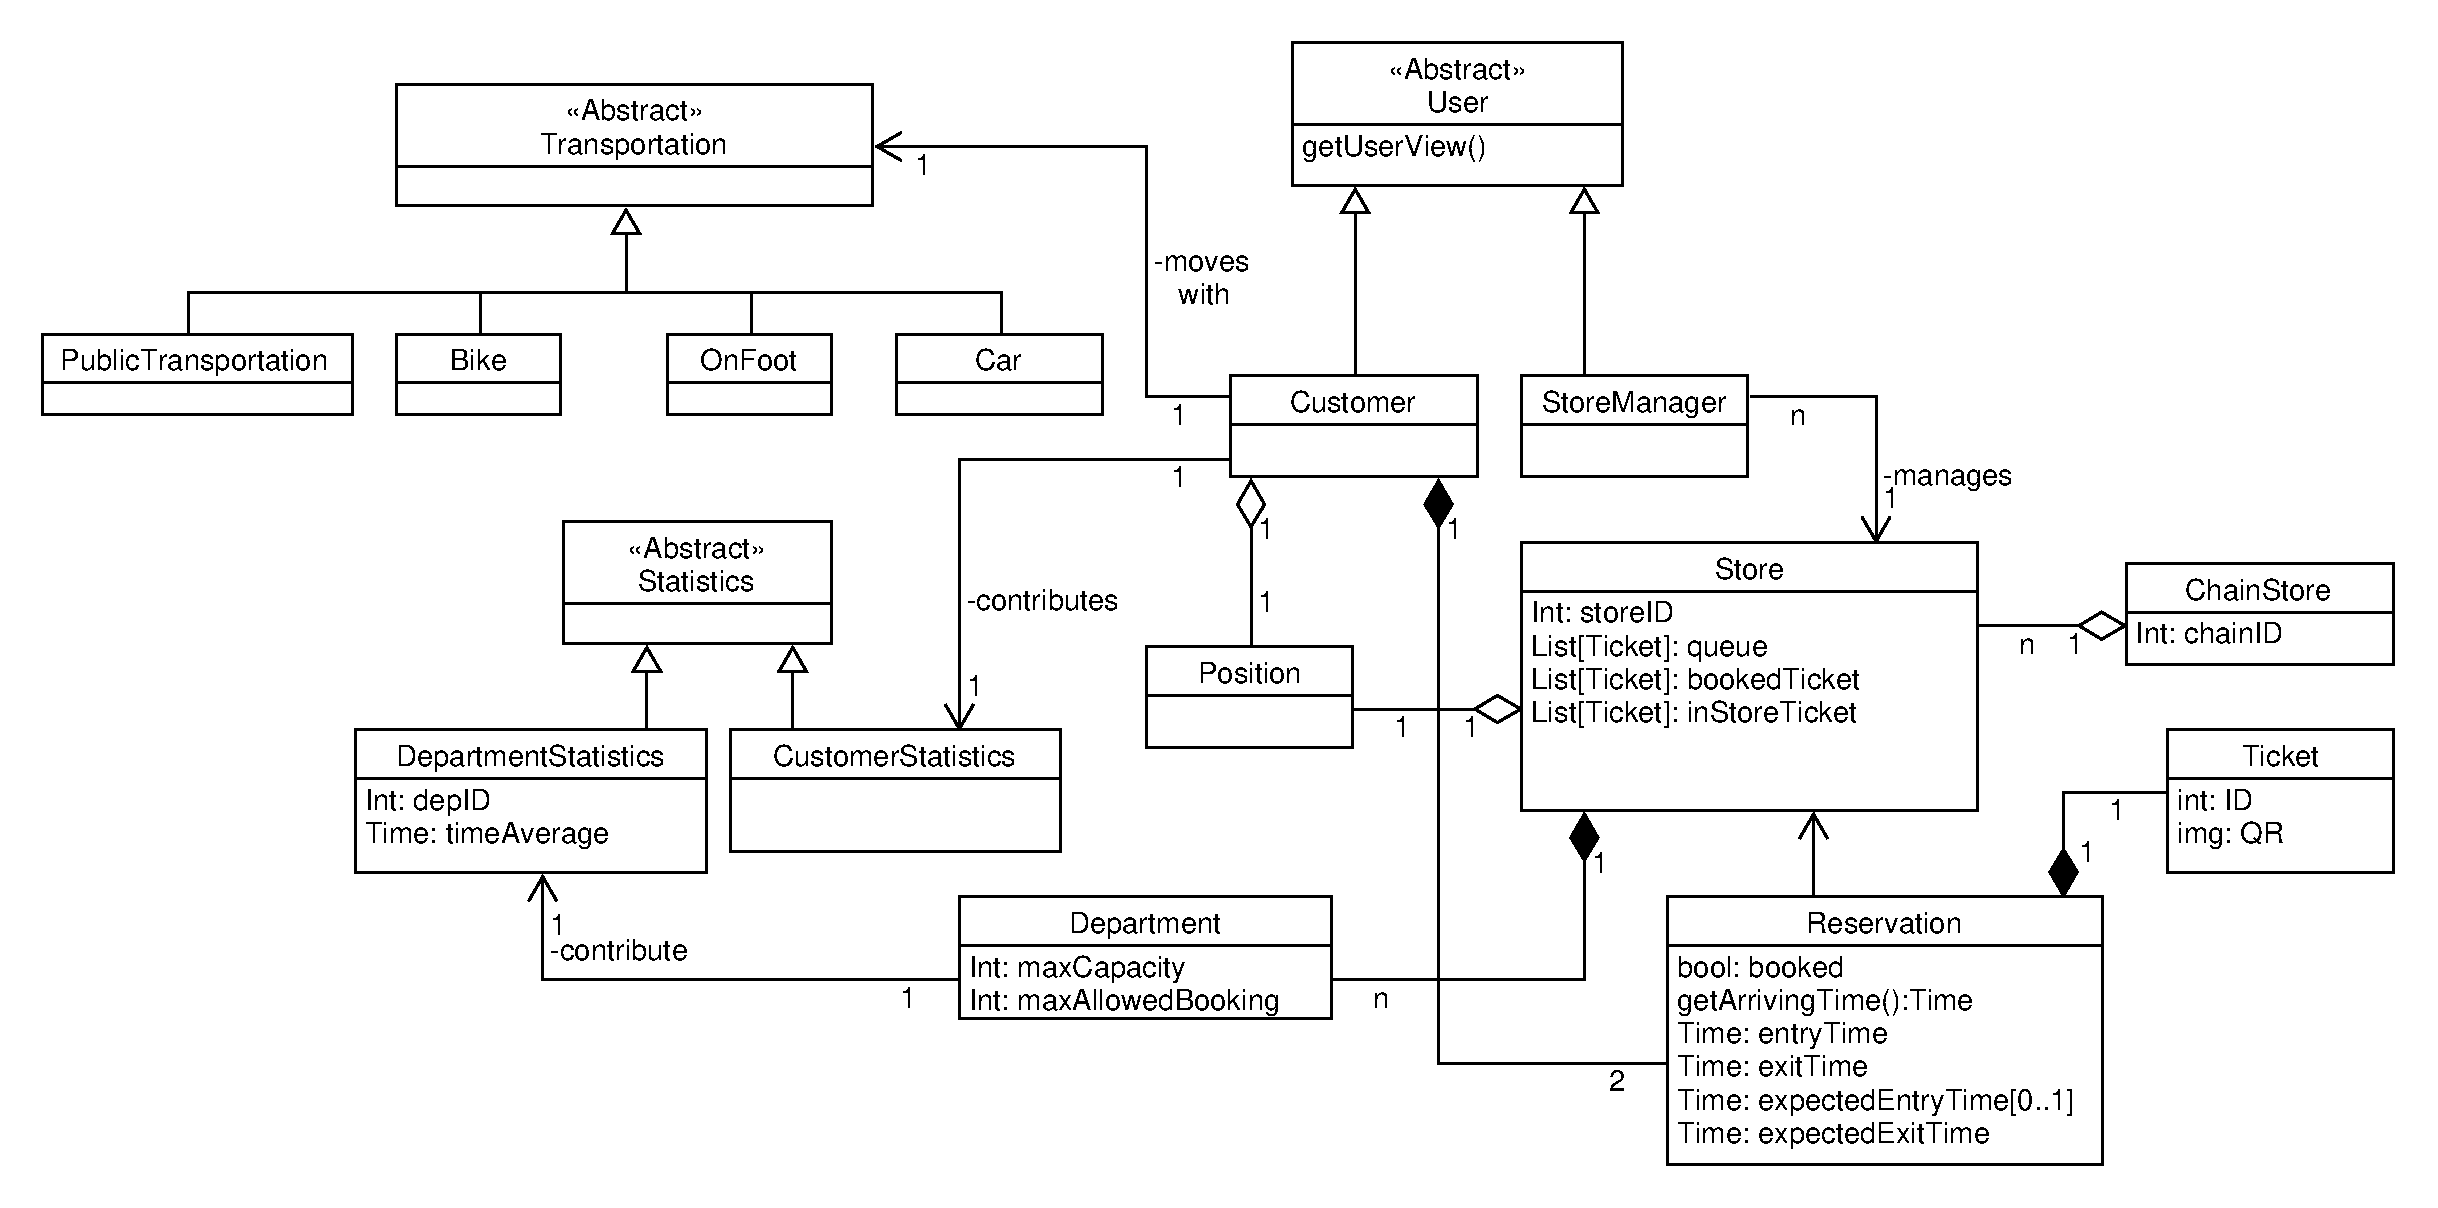
\includegraphics[scale=0.43, angle=90, trim= 0 0 0 -5cm]{ClassDiagrams/classDiagram.pdf} \\
				\caption{\emph{UML Class Diagram}}
			\end{adjustwidth}
		\end{figure}
	
		\newpage
		
		\subsubsection{State Charts}
		
		Now we are going to examine some essential aspects of the application, modelling their behaviours and evolution over time through adequate state diagrams, which are reported below. All the state machines are supposed to start at store opening, and to stop at closing.
		
		\begin{figure}[!h]
			\centering
			\hspace*{-1.9cm}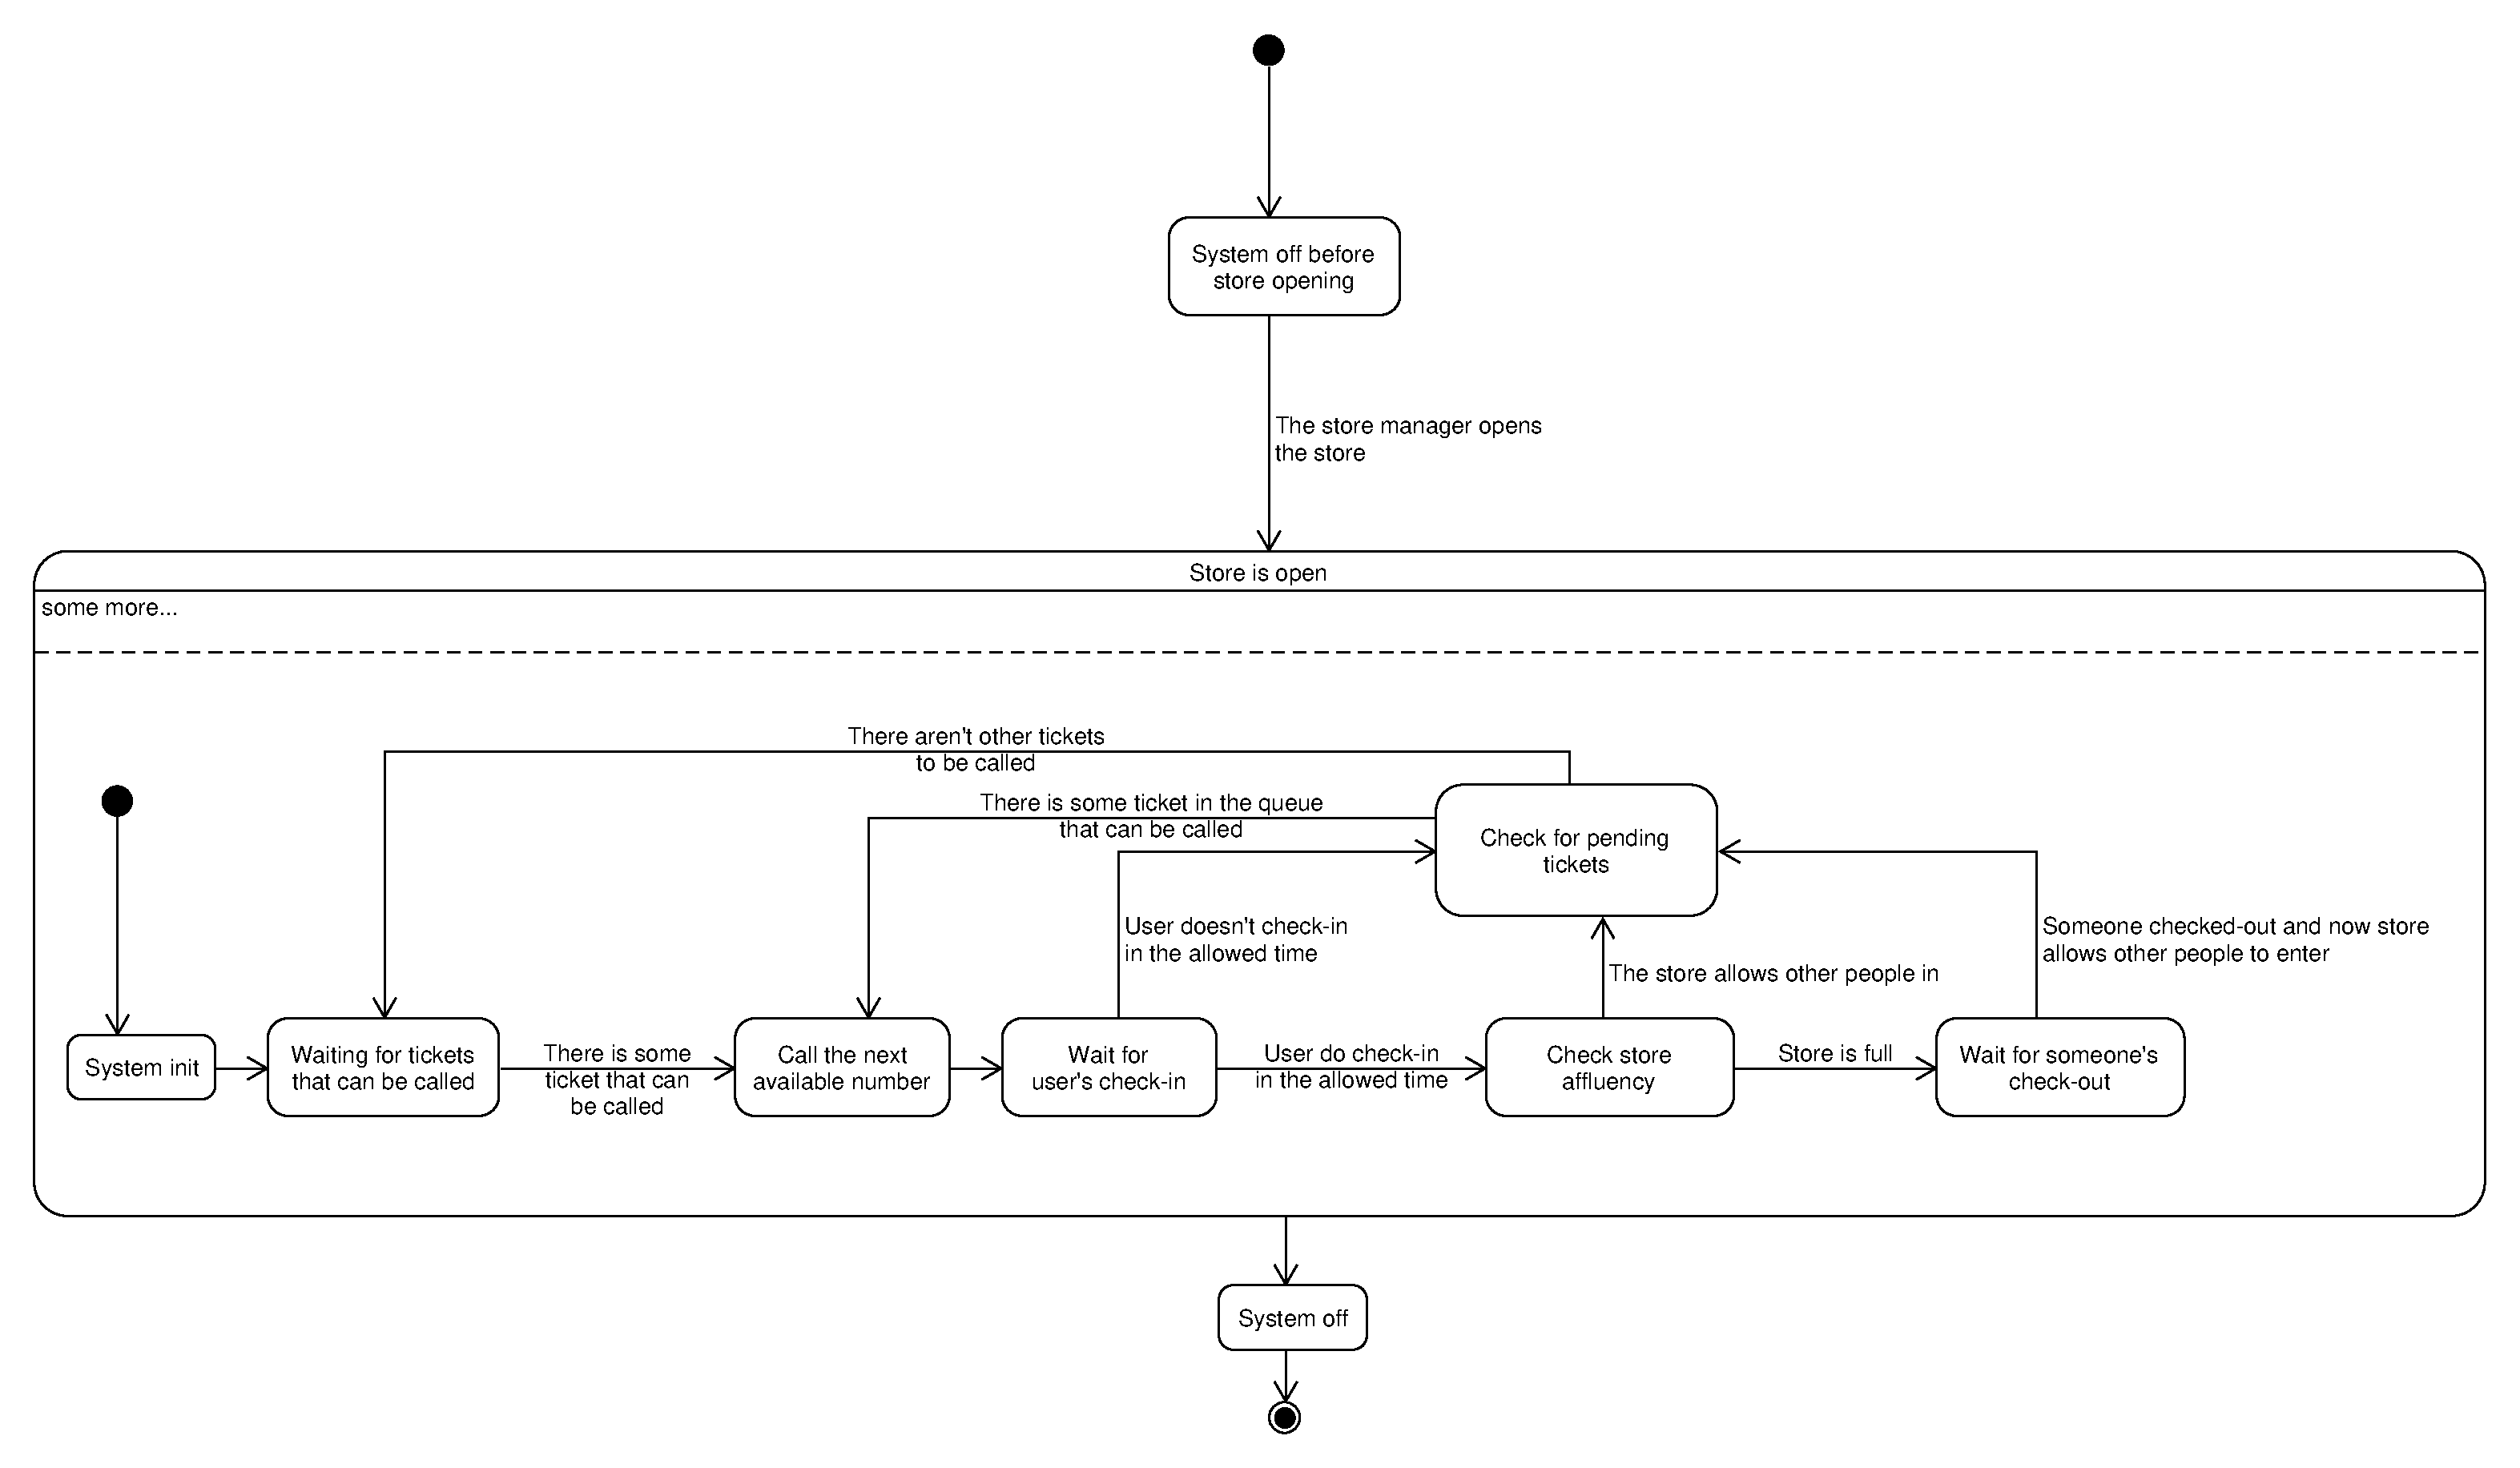
\includegraphics[scale=0.32]{StateCharts/number_calling_system.pdf} \\
			\caption{\emph{Number calling system}}
		\end{figure}
	
		When the store manager opens the store, the system initialize itself, clean up the queue if some ticket remained from the previous day, initialize the queue with the booked tickets, and waits for some ticket that can be called. After a ticket is available to be called, the system notify in some way (e.g. through a store employee) that now certain ticket is allowed to enter the store. At this point, the system waits for the scan of the associated \emph{QR Code}. If the customer doesn't check-in in the assigned time, the system discard the ticket and checks if there are other available tickets. If so, it returns in the calling number state; else, it will wait for an eligible ticket to be called. If the user, otherwise, scan his \emph{QR Code} in time, the system checks the affluence of the store. If it's full, the system will wait for someone's check out, in order to check if some ticket can be called. Else, if the store isn't full, the system doesn't have to wait for a check out to check if there is some ticket eligible to be called. When at some time the store manager will close the store, the system begins its shutdown procedure.
		
		\bigskip
		
		\begin{figure}[!h]
			
			\centering
			\hspace*{-0.0cm}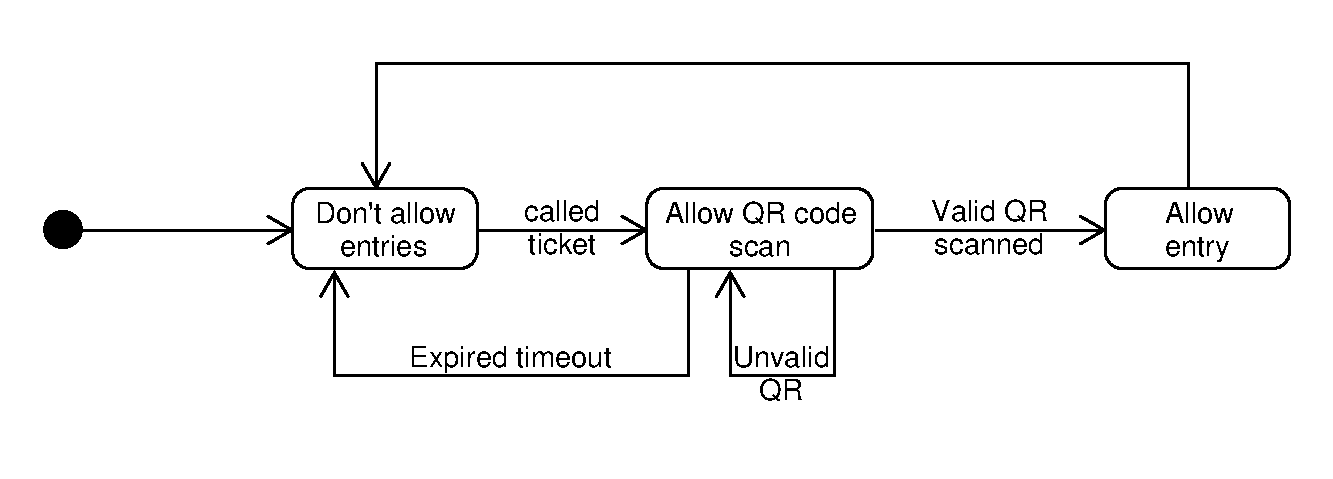
\includegraphics[scale=0.54]{StateCharts/qr_scanner_uml.pdf} \\
			\caption{\emph{QR Code scanner state machine for entering the store}}
			
		\end{figure}
		
		The system doesn't allow entries until a ticket is called by the system described above. Then, the \emph{QR Code} reader waits for a \emph{QR Code} to be scanned. When a \emph{QR Code} is passed under the optical reader, the system checks if it's a valid one; if so, allows the entry, otherwise notify the wrong \emph{QR Code} and continue waiting for the right one. If the valid \emph{QR Code} isn't scanned in time, the system blocks the entry, discards the current called ticket and waits for the next reservation to be called. Otherwise, if the valid \emph{QR Code} is scanned in time, the system allows and registers the entry.
		
		\bigskip
		
		\begin{figure}[!h]
			
			\centering
			\hspace*{-1.9cm}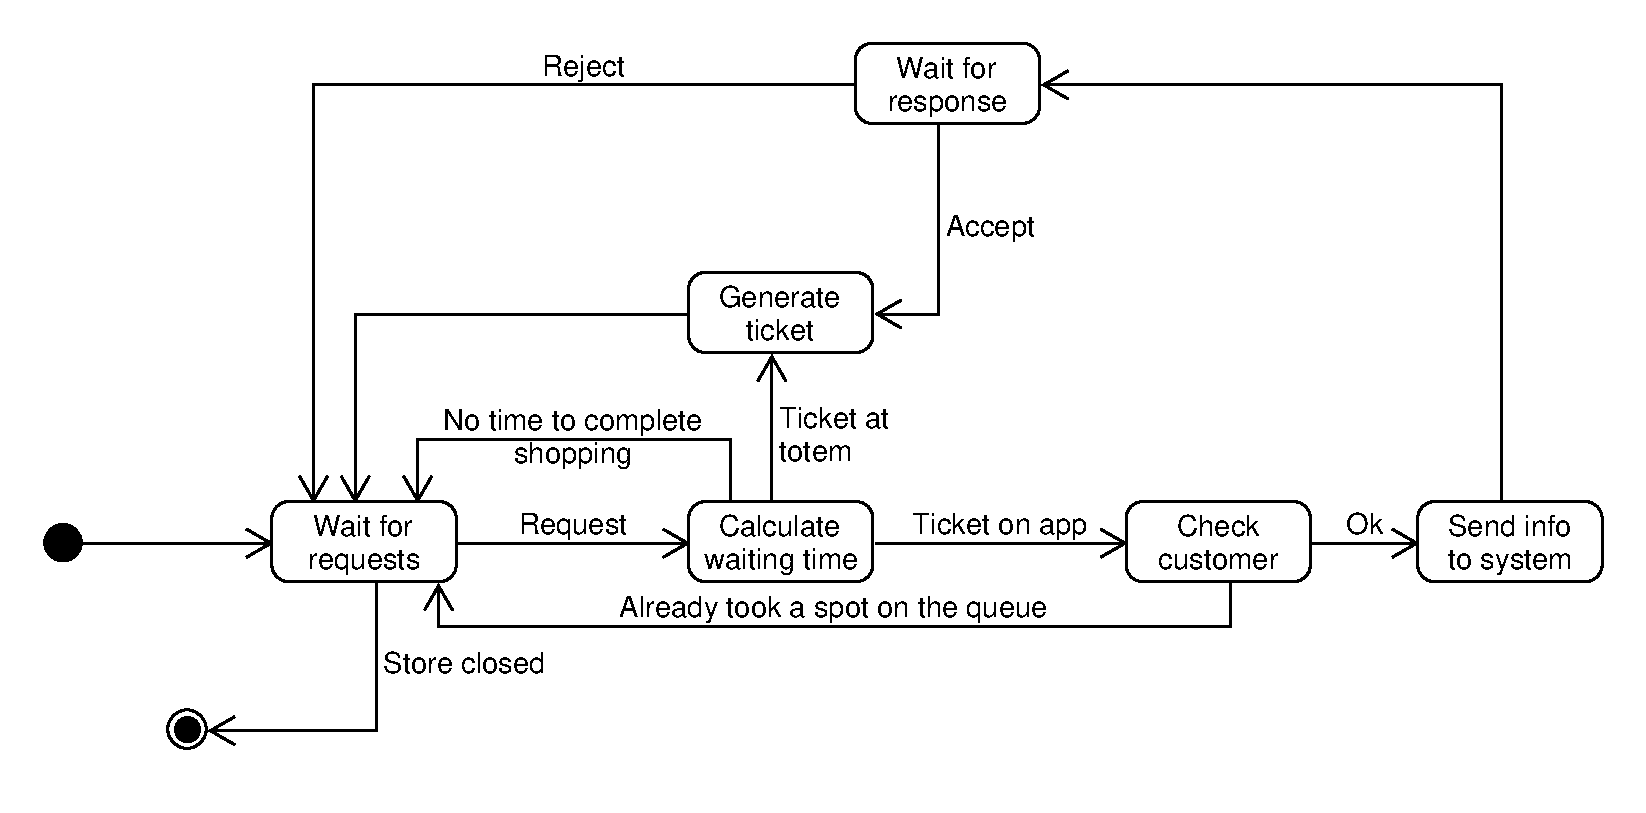
\includegraphics[scale=0.55]{StateCharts/ticket_generation_system.pdf} \\
			\caption{\emph{Ticket generator system state machine for entering as soon as possible in the store}}
			
		\end{figure}
	
		Here is described the state machine of the generation of ticket to enter as soon as possible in the store. First, the system calculates the waiting time. Then, if there is time to complete shopping and the request arrives from a totem, the reservation is issued; else, if the reservation process happens on the app, and there is time to complete shopping, if the customer isn't already on the queue, the system elaborates data and two things happen, depending on waiting time: if it's low, an automatic response is sent, and the reservation processed; else, when the \emph{ETA} is high, it's waited a response from customer, that can follow some suggestions from the system, or maintain his preference. Another situation may happen: there is no time to complete the shopping, since the customer may require to shop more time than how much is missing to the store closure. In this case, the ticket is not issued.

	\newpage
	\subsubsection{Scenarios}
	
	{\bfseries Scenario 1: User without application} \\
	Marta is a university student unfavorable to consumerism and for this reason she does not have a smartphone. She go to her favorite store to do shopping and thanks to our system she can still book a place in the queue to enter in the store. To do this, she just go to the totem placed near the supermarket and fill in the reservation with the requested data, that is the departments she intends to visit and an estimate of the time spent inside the store. In this way, the system will queue her to enter as soon as possible, providing her with an estimated entry time. Knowing this, Marta can still do other activities before being called to enter the store, so as not to create crowds at the store exit. As with the app, Marta has to scan the ticket at the  entrance and exit. In this way the system can manage the queue and reservations. \\ \\
	{\bfseries Scenario 2: Fake \emph{QR Code}} \\
	Jonathan arrives at the store and notices that he has many people in line before him. Jonathan is not a very patient guy, so having kept another \emph{QR Code}, he tries to skip the line trying to scan it. The system recognizes that the \emph{QR Code} is not valid, therefore it does not allow Jonathan to enter the store, forcing him to respect the queue. \\ \\
	{\bfseries Scenario 3: User books from the application} \\
	Adalgiso must go shopping but does not want to wait a long time outside the store and wants to be sure that he can enter the moment he arrives. So, he opens \emph{CLup} on his smartphone, sets up a preferred means of transport and begins a reservation. He selects the store, the departments he wants to visit and the estimated time. Once the booking is complete, the app will send the notification to Adalgiso, inviting him to depart from his position to go to the store in time. When he will arrive, his number will be called shortly.\\ \\
	{\bfseries Scenario 4: Store manager have to smartly manage accesses} \\
	Apu is a store manager whose work is made more difficult by the current pandemic, since he has a small shop and no ways to manage crowds. Thanks to our application, now Apu is able to avoid assembles in front his store, he doesn't worry anymore about the number of people inside the store, and thanks to the real time statistics, he is able to regulate better the number of allowed people and booked ones for each department of his small store.\\\\
	{\bfseries Scenario 5: Arrives near the store closing} \\
	Caterina arrives at the store near the closing, but her shopping would last over the closing time. To avoid that she waits in vain, a ticket isn't issued. So, Caterina reduces the departments that she should visit. She may have time to complete the shopping, but she have to hope that the crowd runs fast, or her ticket won't be called. Since there are possibilities to enter, the ticket is issued, but she is alerted that may not be able to enter the store.
	\newpage
	\subsection{Product Functions}
		
	In the previous chapter there were introduced, sketchily, the main features of the software in order to understand, in general, its functioning. Alternatively, in this section will be illustrated and described accurately all the functions that the software allows to do.
	
		\subsubsection{Getting a ticket}
		
		In order to manage the accesses to stores' buildings, it's used a system based on the "call of numbers". Each user in the queque has a unique \emph{ID}, and when his number is called (eg. by a store employee), the user is authorized to enter. This mechanism works also for the booking feature, since the system generates a number that won't be called until the beginning of the time slot selected by the user, in according to the previously reported criteria. Users can get a ticket both on the application and at a totem installed at the entry of the store (obviously, on the app users are required to select some specific store of their preference from a given list, sorted by the nearest one from the position obtained from the \emph{GPS}). With the generation of the ticket, the user will get both an \emph{ID} and a \emph{QR Code} associate to it, to be scanned at the enter of the store. When getting a ticket on the application, users must be logged in with their credentials (if not, they must register at the services), while at the \emph{totem} they can simply get the ticket without giving any data. At the store's \emph{totem}, customers can only get a ticket to enter as soon as possible. On the app, customers can see at any moment their reservations, along with the expected calling time, and the time needed to reach the store by the preferred mean of transport selected in the settings. \emph{ID} and \emph{QR Code} are always available offline, while the other informations need an internet connection and a \emph{GPS} signal to be updated (without them, inaccurate data may be visualized). On app, customers get a digital ticket with its associated \emph{QR Code}; at \emph{totem}, the ticket and the \emph{QR Code} are printed. On both of them, there is displayed the expected time of call, based on the queue situation at the ticket issuing. This time is indicative, and can decrease if some customers doesn't enter the store. In case it's estimated that a reservation can enter the store after store's closing time, a warning on tickets is printed, along with the time store closes. This reservations are always generated, since, as previously explained, customers may give up line, reducing waiting times. Making the reservation, the user can indicate the department in which he is interested, and using the app can decide both to have a ticket to enter as soon as possible in the store or to plan his visit. 
		
		\subsubsection{Calling process}
		
		The process to admit people without a booking in the store follows a \emph{FIFO} logic: the first one that got a ticket, is the first to access the store. When called, a person is authorized to access the store. To register his entry, he is requested to check-in at the entry in a certain amount of time. Tickets related to the \emph{FIFO} queue can be called as soon as the requested zones are available, and tickets related to bookings can be called only after the start time of the booked time slot, and will be called around this time, when all the booked zones become available (to avoid starvation on calling bookings, other tickets requesting at least one booked zone won't be called until the booked tickets enters the supermarket). Obviously, in the queue may happen to be some reservations that needs to stay inside the store after the closing time. In such cases, these tickets are not called.
		
		\subsubsection{Check-in/Check-out}
		
		At the store entries and exits, users have to scan their \emph{QR Code} to respectively Check-in and Check-Out in the supermarket. If someone doesn't check-in in a prefixed amount of time, definable by the store manager, he'll lost his turn in the queue. \emph{QR Code} scan is required for some important reasons: register someone's entry in the store for contact tracing purposes, to know the actual affluence of the store, to mine statistics and to check that the person entering the store is the one called, to avoid stoles of turns.
		
		\subsubsection{Plan a visit}
		
		The app allows customers to plan a visit in a store of their preference. At the end of the process of getting a reservation, customers can select to plan their visit to the store. After inserting the preferred day (in a 7 day range from the day of the request), and available the time needed by customer to complete the shopping, the app will propose customer some time intervals in which he can enter the store, to satisfy both estimated time of permanency and the maximum simultaneously bookings allowed in a department. 
		
		\subsubsection{Managing store and single departments}
		
		Store managers are able to modify some settings of the store. It's possible to have different parameters for each day of the week. Regarding the entire store, the editable parameters are:
		\begin{itemize}
			\item The available departments (with the constraint of at least one department)
			\item For each day of the week, if the store is closed or opened, and if opened the working hours;
			\item The maximum allowed bookings per week from a single customer;
			\item The maximum waiting time between a ticket calling and its scan at the entry
		\end{itemize}
	
		Instead, for each department, the store manager is able to define:
		\begin{itemize}
			\item The maximum number of simultaneous customers allowed in it;
			\item The maximum number of simultaneous booked customers allowed in it.
		\end{itemize}
	 When a department setting is changed, the already made bookings will be rescheduled at the first available entry time, notifying each user of the change. The priority is to allow customers that booked the visit to enter in the same day, if it's possible. If any time on the same day can be allocated, the bookings will be cancelled and the customers notified. For tickets got from the \emph{totem}, customers will be alerted from a store assistant of the possible delays. A such operation may reduce in the already booked days the number of admitted non-booked clients. 
	 The app also allows store managers to see the real time situation in their stores.
	
		\subsubsection{Notify users}
		
		If some account have pending reservations, depending on the position of the customer (retrieved by \emph{GPS}), and the preferred option of reaching the selected store (eg. on foot, by car or public transport), the app will notify the customer when he should depart from his position, by the selected mean, to arrive in time to enter the supermarket, without losing its turn and avoiding long waiting times. Notice that not all of the moving options may be available in all the places, since it depends on the used map service. This service is obviously available only with the internet connection and the GPS active.
		
		\subsubsection{Cancel and modify reservations}
		
		If the user can not reach the store in time, he can decide to cancel or modify the booked visit, or to leave his spot on the queue. So, the system deletes the customer from the queue (if inside it) and rearrange the last one. Also store managers are able to perform the same operations on customers' reservations. 
		
		
		\subsubsection{Infer waiting time from users}
		
		The system can infer the average time spent by a user in the supermarket using previous visits as informations. If the client is taking a spot on the queue or booking a visit on the app, he will be asked to insert a reasonable duration of his visit; however, he can let the application to manage this parameter for him. If there aren't enough informations on the specific client, the app will infer this time from other clients' visits that did a similar shopping. Otherwise, it will find the information from client's previous visits. The same thing happens at the totem, where or the client inserts an estimation, or the system will use the whole stored informations.
		
		\subsubsection{Allow a fair management of the accesses}
		The system is able to manage in a fair way the process of releasing tickets and accepting bookings. In fact, depending on the store's closing time, and other informations in its possession, such as the number of people in queue, the estimated time of permanency and some other statistics, it's able to notify customers about risk to not enter the store, if any, and to block the generation of new tickets, if there isn't enough time to do the shopping. The store manager is able to decide the maximum number of contemporary bookings allowed in each department, to avoid that it's really difficult to enter the store without a booking. Moreover, a user can make a limited number of bookings per week, and on app can't simultaneously take more than one spot on a queue. \\
		
		\subsubsection{Make suggestions}
		\emph{CLup} is able to suggests customers better options than the chosen ones. In fact
		\begin{itemize}
			\item If the customer is taking a spot in the queue, and the waiting times are really high, depending on customer's \emph{GPS} position and the preferences inserted in the process, some alternative stores with lower waiting times (where it's considered also the time needed to reach store's position) may be proposed.
			\item If the customer is booking a visit, and the proposed time intervals are not of his interest, it's possible to request, from the same page, suggestions on other near stores with more booking possibilities.
		\end{itemize}

	\bigskip
	
	\subsection{User Characteristics}
	
	\emph{CLup} gives access to two different sets of functionalities to make easier the life of two categories of users:
	
	\bigskip
	\begin{itemize}
		
		\item {\bfseries Customer}: \emph{Covid-19} made challenging going to a store in the right time to avoid crowds and high waiting times. So, for customers, the aim of the application is to make less frustrating going at a supermarket, helping them to plan a visit, to take a spot on queue before exiting home and to be alerted when they should depart from home. \\
		
		\item {\bfseries Store Manager}: The pandemic made life harder also for store managers. Now, with this system they can manage in an almost automatic and safe way the access to their stores. \\
		
	\end{itemize}

	\subsection{Assumptions, Dependencies, Constraints}
	
	\bigskip
	
		\subsubsection{Domain Assumptions}
			
			\begin{center}
				
				\rowcolors{2}{}{gray!20}
				\rowcolors{1}{gray!20}{white}
				\renewcommand{\arraystretch}{2.5}
				
				\begin{adjustwidth}{-2.4cm}{}
					\begin{tabular}[h!]{|m{3em}|m{37em}|}
						
						\hline
						\xrowht{5pt}
						\centering DA1 & Date and time on the devices on which \emph{CLup} runs are always correct \\
						\xrowht{5pt}
						\centering DA2 & Internet connection works always without errors \\
						\xrowht{5pt}
						\centering DA3 & Customer’s position retrieved by \emph{GPS} is accurate \\
						\xrowht{5pt}
						\centering DA4 & In each store, different objects belonging to the same category are in the same department \\
						\xrowht{5pt}
						\centering DA5 & Totems always work properly and are not damaged \\
						\xrowht{5pt}
						\centering DA6 & The customer’s smartphone screen is not damaged and the \emph{QR Code} is readable \\
						\xrowht{5pt}
						\centering DA7 & The \emph{Maps API} always calculate the optimal route \\
						\xrowht{5pt}
						\centering DA8 & Every store has a unique name and address combination \\
						\xrowht{5pt}
						\centering DA9 & \emph{QR Code} readers are always working \\
						\xrowht{5pt}
						\centering DA10 & The store capacity inserted by store manager is always correct \\
						\xrowht{5pt}
						\centering DA11 & Customer tries to respect their estimate, without remaining over time \\
						\xrowht{5pt}
						\centering DA12 & Each customer scans his \emph{QR Code} at the enter and enters the supermarket only through the allowed entries. \\
						\centering DA13 & Each paper ticket is not ruined and readable. \\
						\centering DA14 & The working days and hours of the store inserted in the system are corrected\\
						\centering DA15 & All users are ready to depart for the store when they are notified \\
						\hline
						
						
					\end{tabular}
				\end{adjustwidth}
			\end{center}
\newpage

\section{Specific Requirements}

	\subsection{External Interface Requirements}
	
		\subsubsection{User Interfaces}
		
			Customers can use the service using a personal mobile device (eg. a smartphone, a smartwatch or a tablet), or through a totem externally installed at each store to get a spot on the queue. Store managers can also use a device to manage the store. Here there are some mockups of the application. A complete description of all the \emph{UI} will be in the Design Document, attached to this specification document.
			\bigskip
			\bigskip
			\bigskip
			
			\begin{figure}[!h]
				\centering
				\begin{minipage}[!h]{0.4\textwidth}
					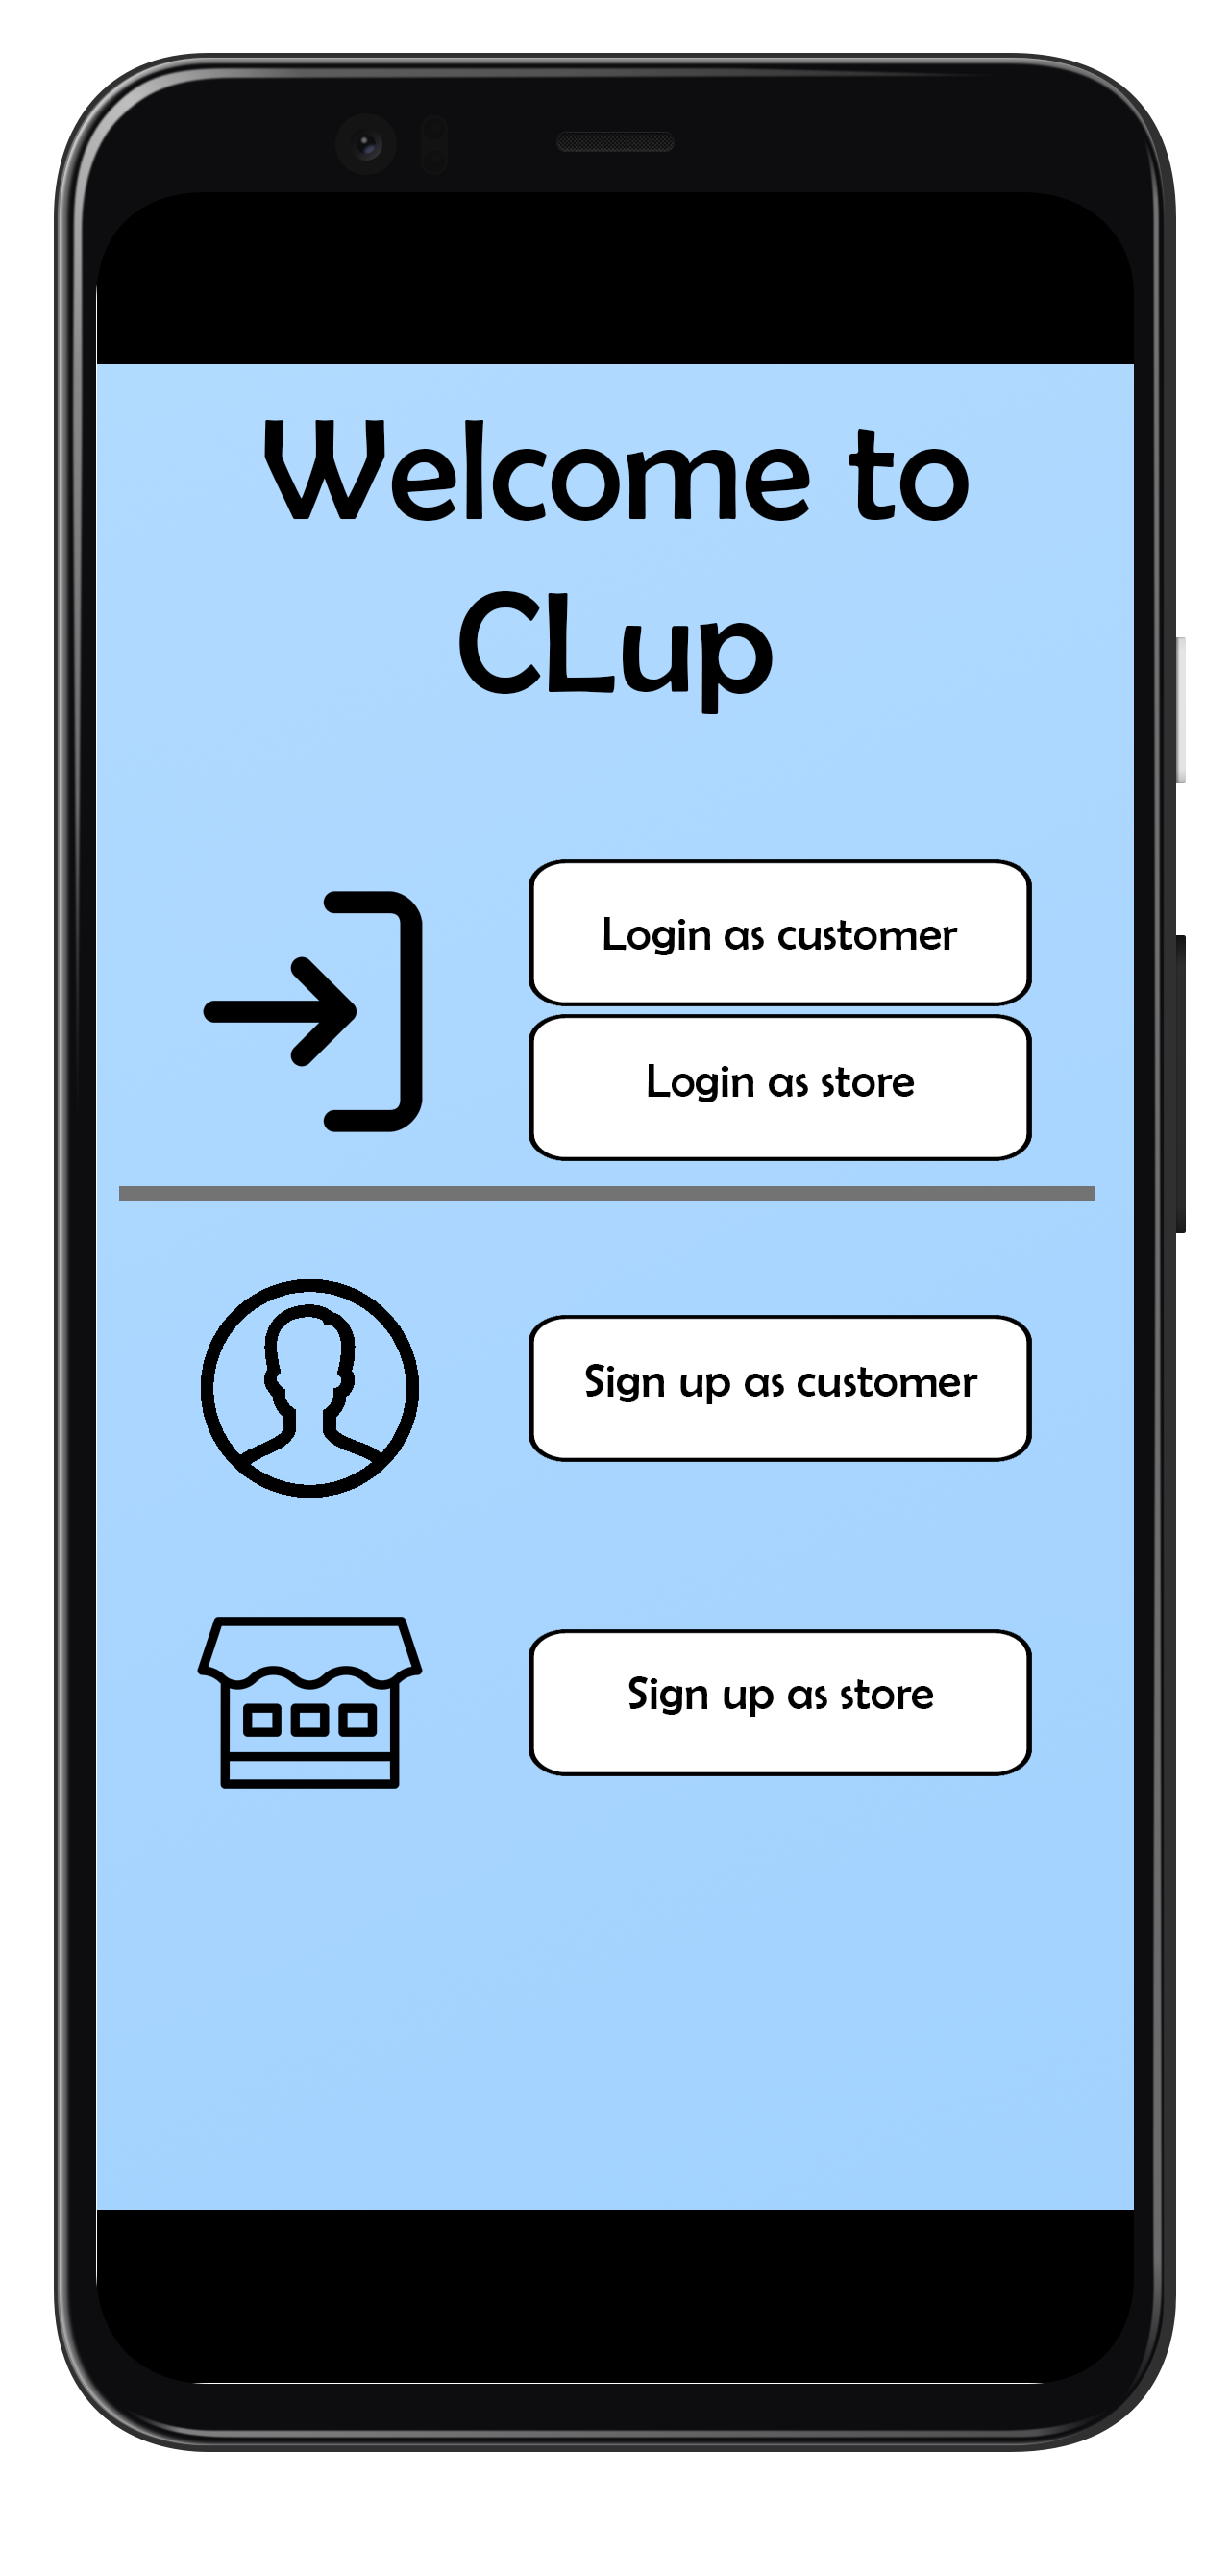
\includegraphics[width=\textwidth]{../Mockups/InitialPage.png}
					\caption{\emph{Home page}}
				\end{minipage}
				\hfill
				\begin{minipage}[!h]{0.4\textwidth}
					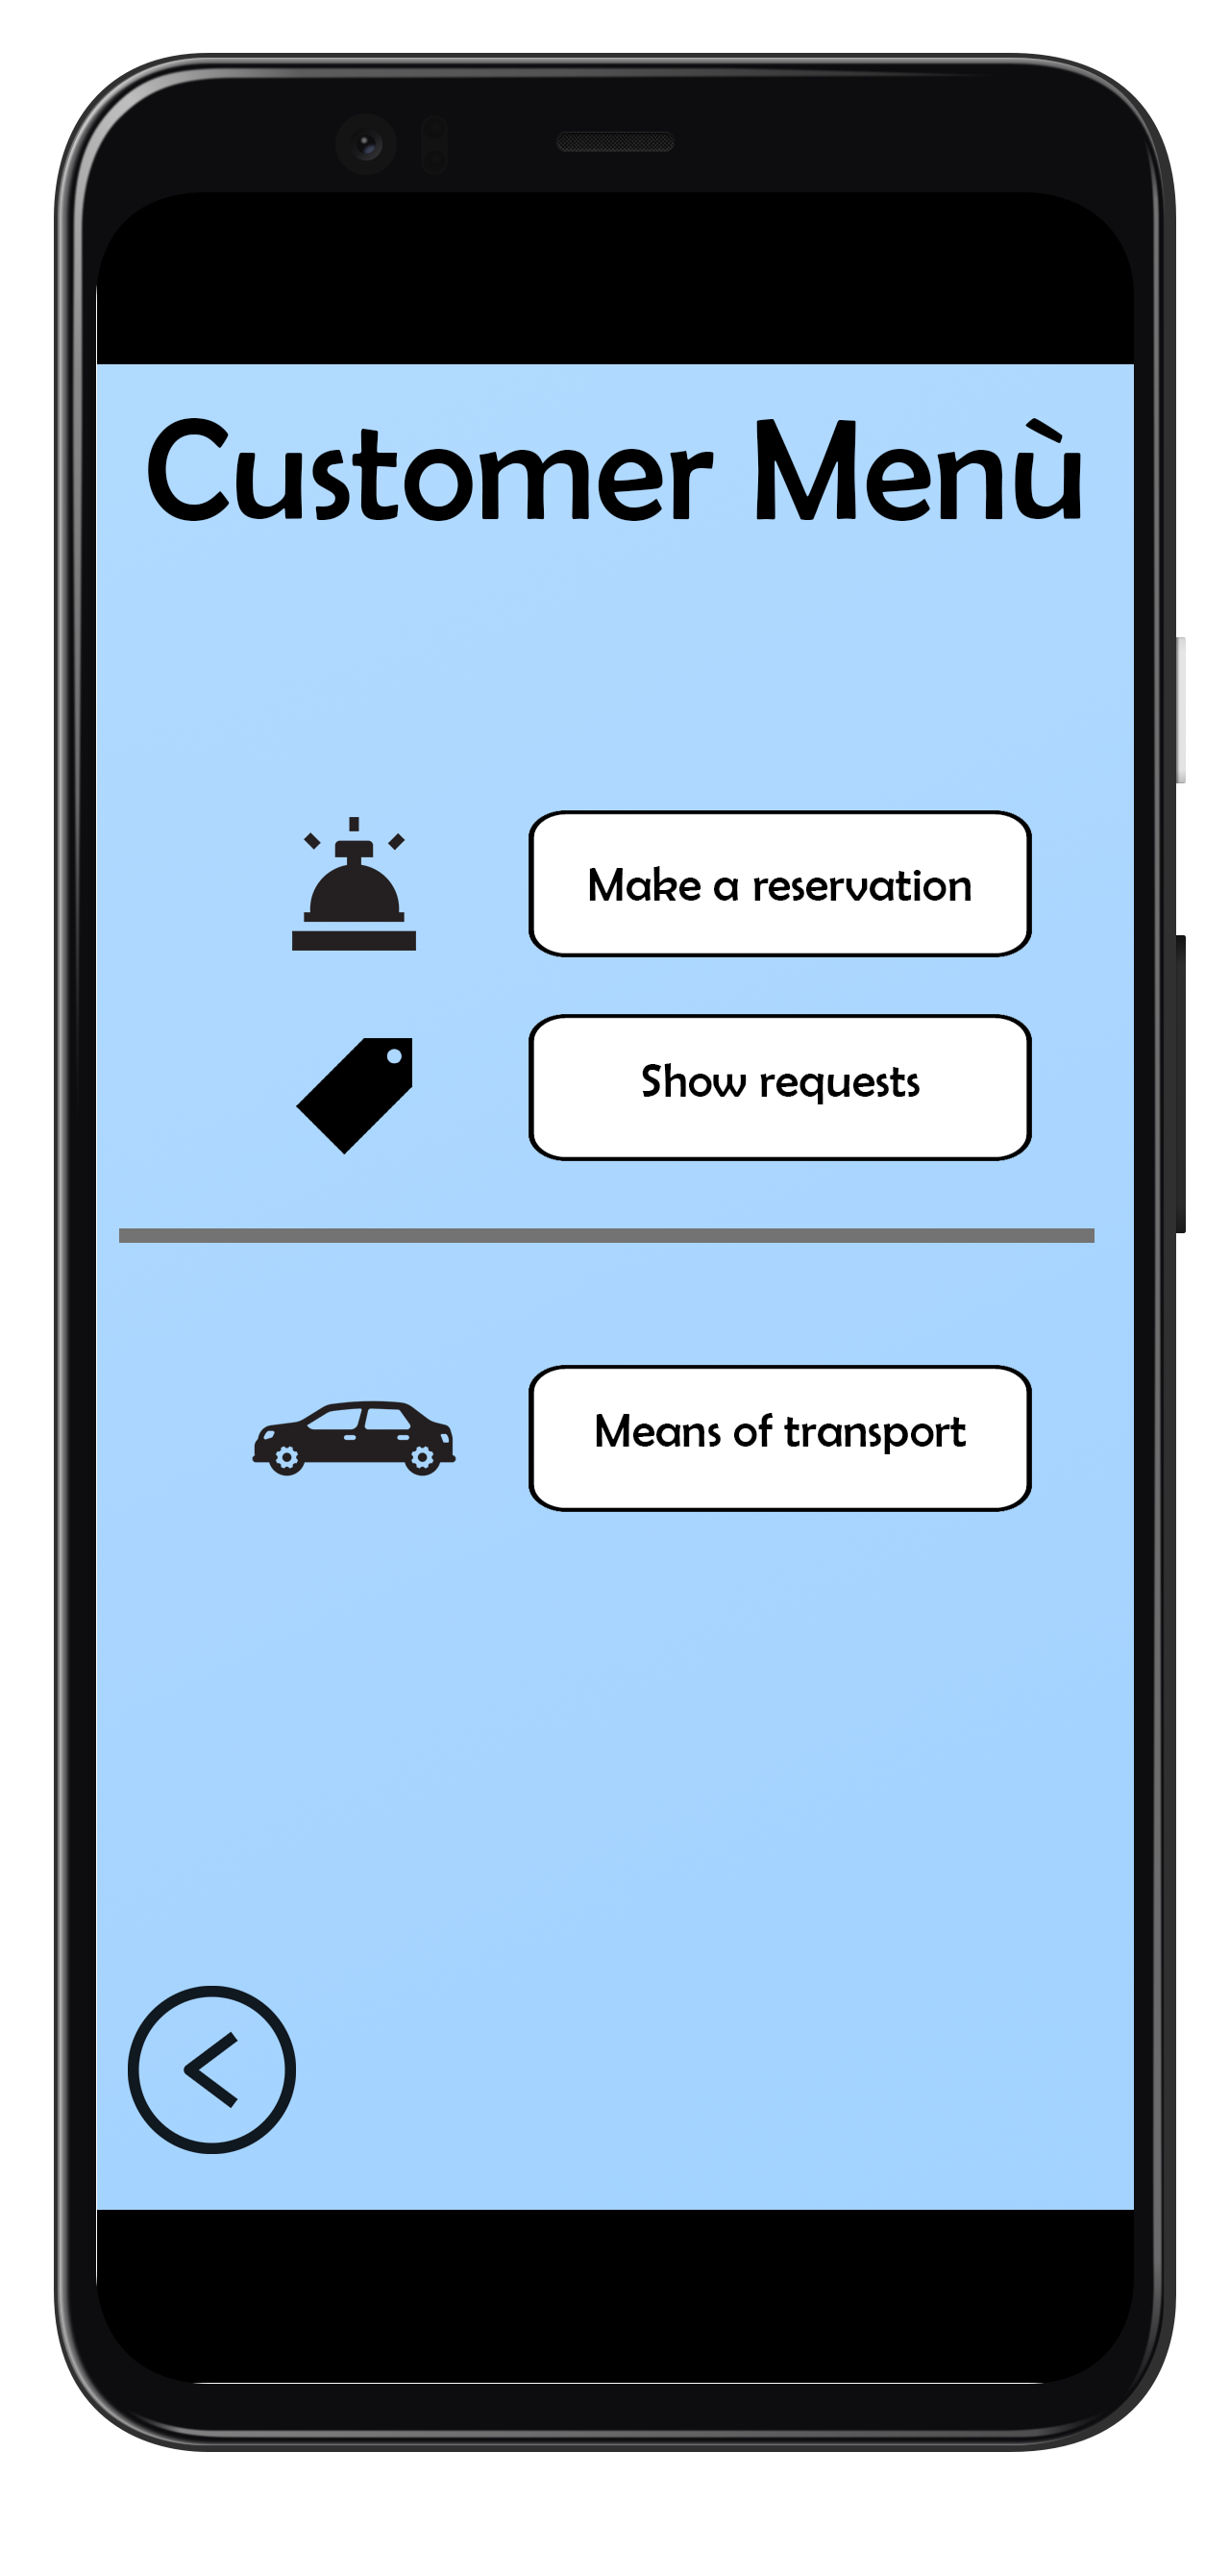
\includegraphics[width=\textwidth]{../Mockups/MenuCustomer.png}
					\caption{\emph{Customer menu}}
				\end{minipage}

			\end{figure}
		
		\newpage
		\begin{figure}[!h]
		\begin{minipage}[!h]{0.4\textwidth}
			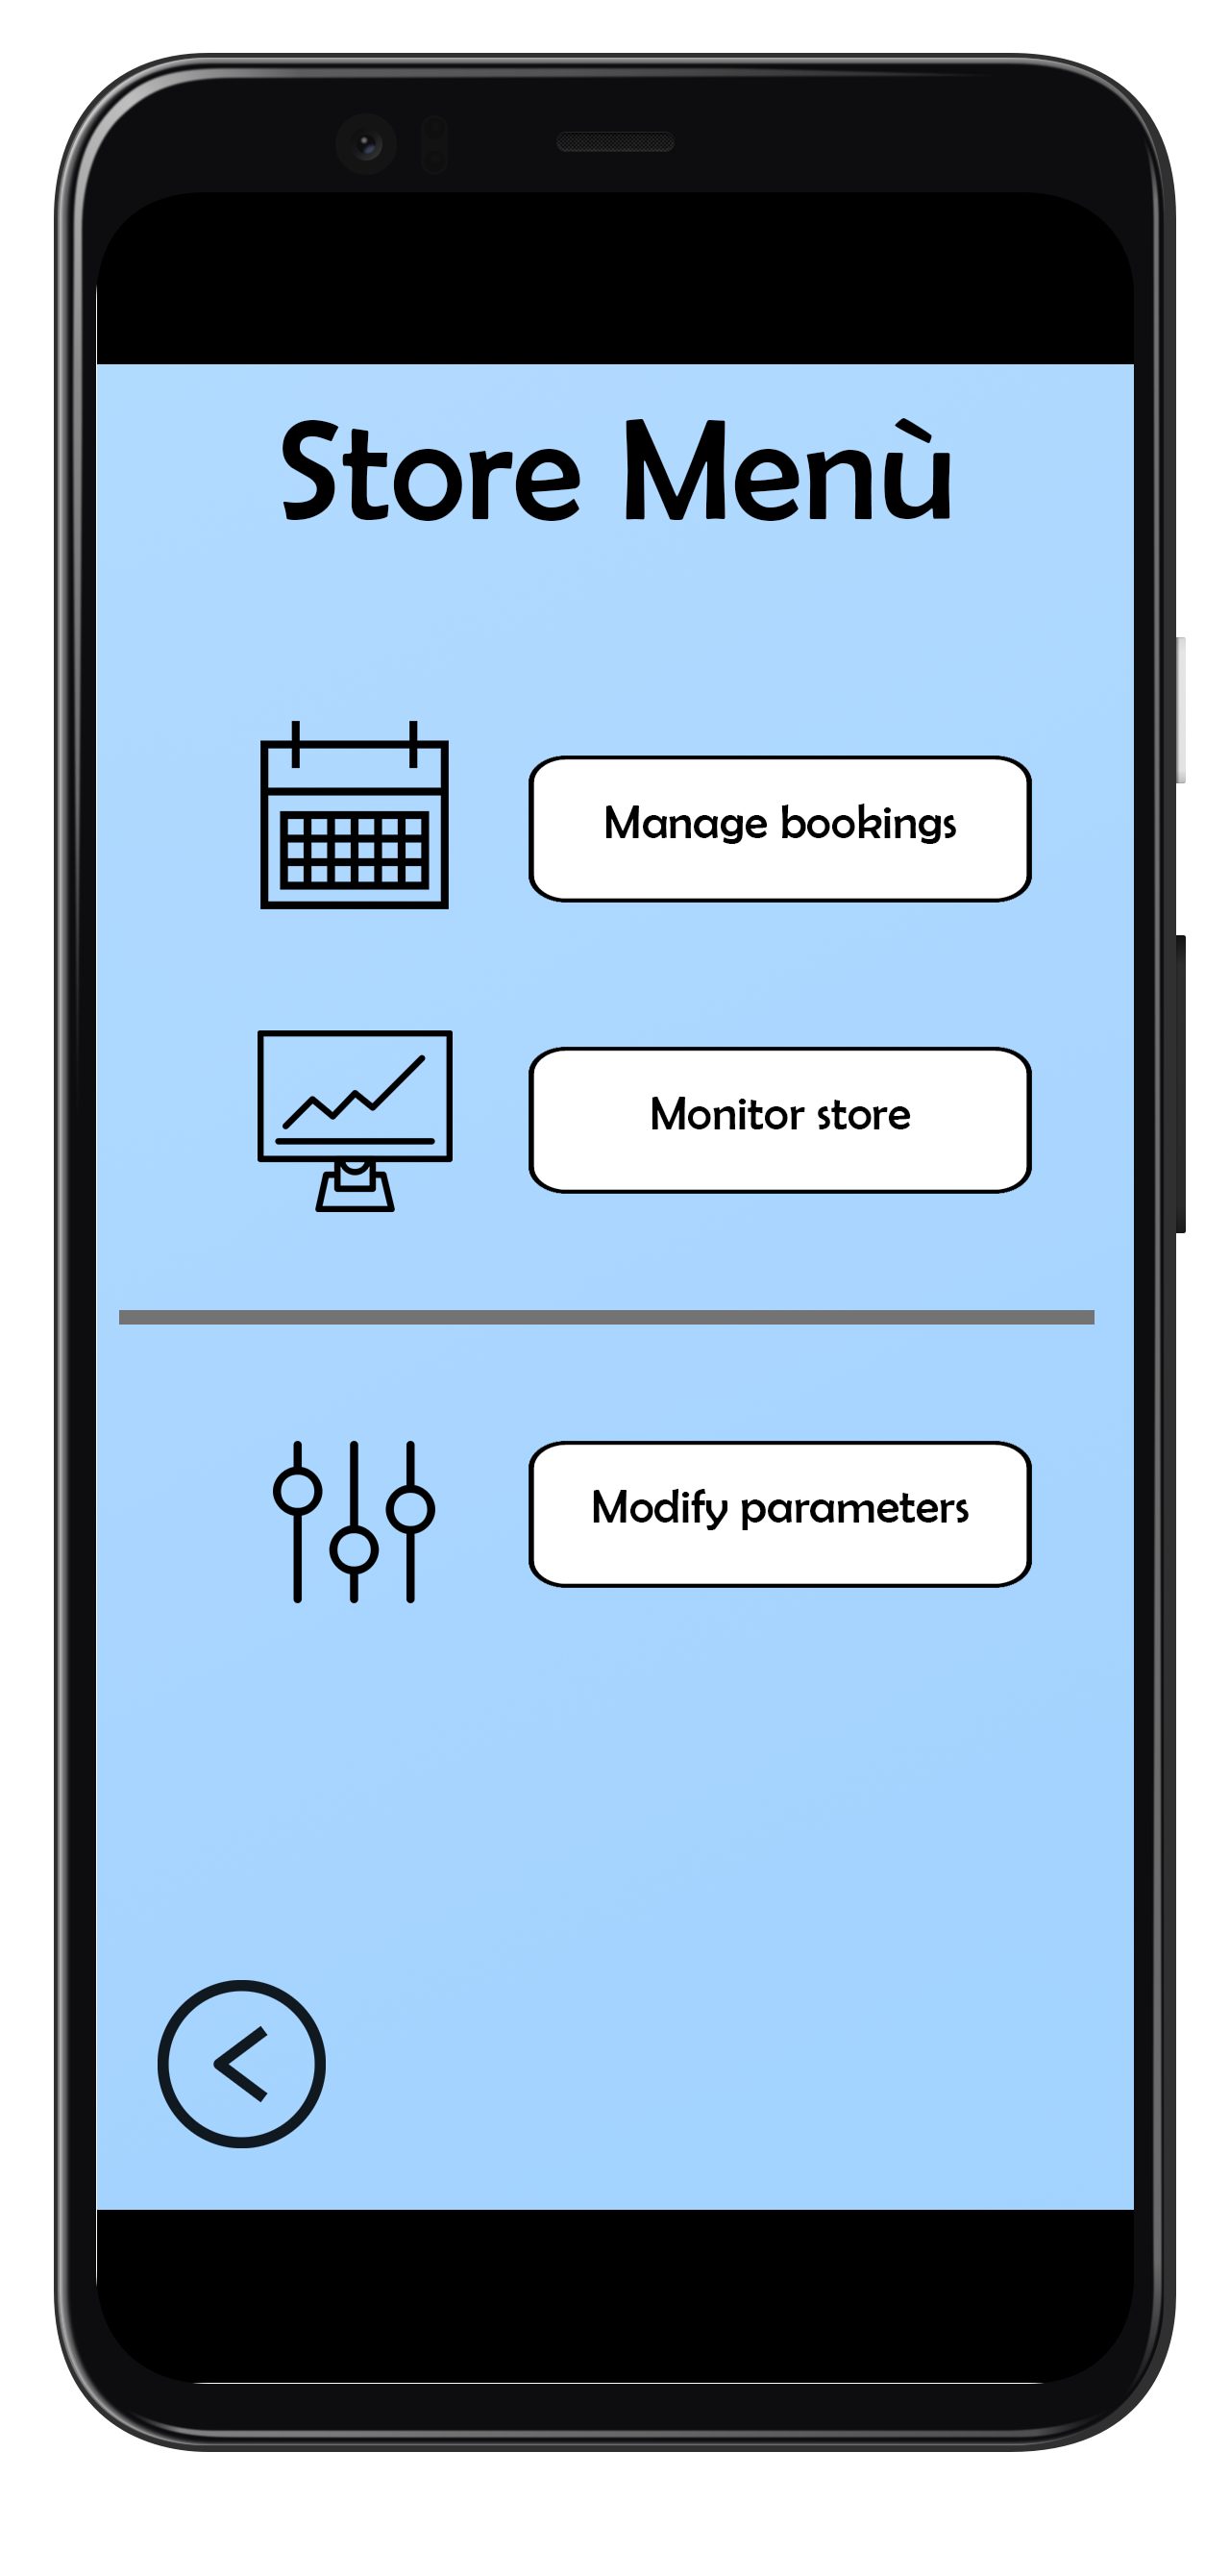
\includegraphics[width=\textwidth]{../Mockups/MenuStore.png}
			\caption{\emph{Store manager menu}}
		\end{minipage}
	\hfill
		\begin{minipage}[!h]{0.4\textwidth}
			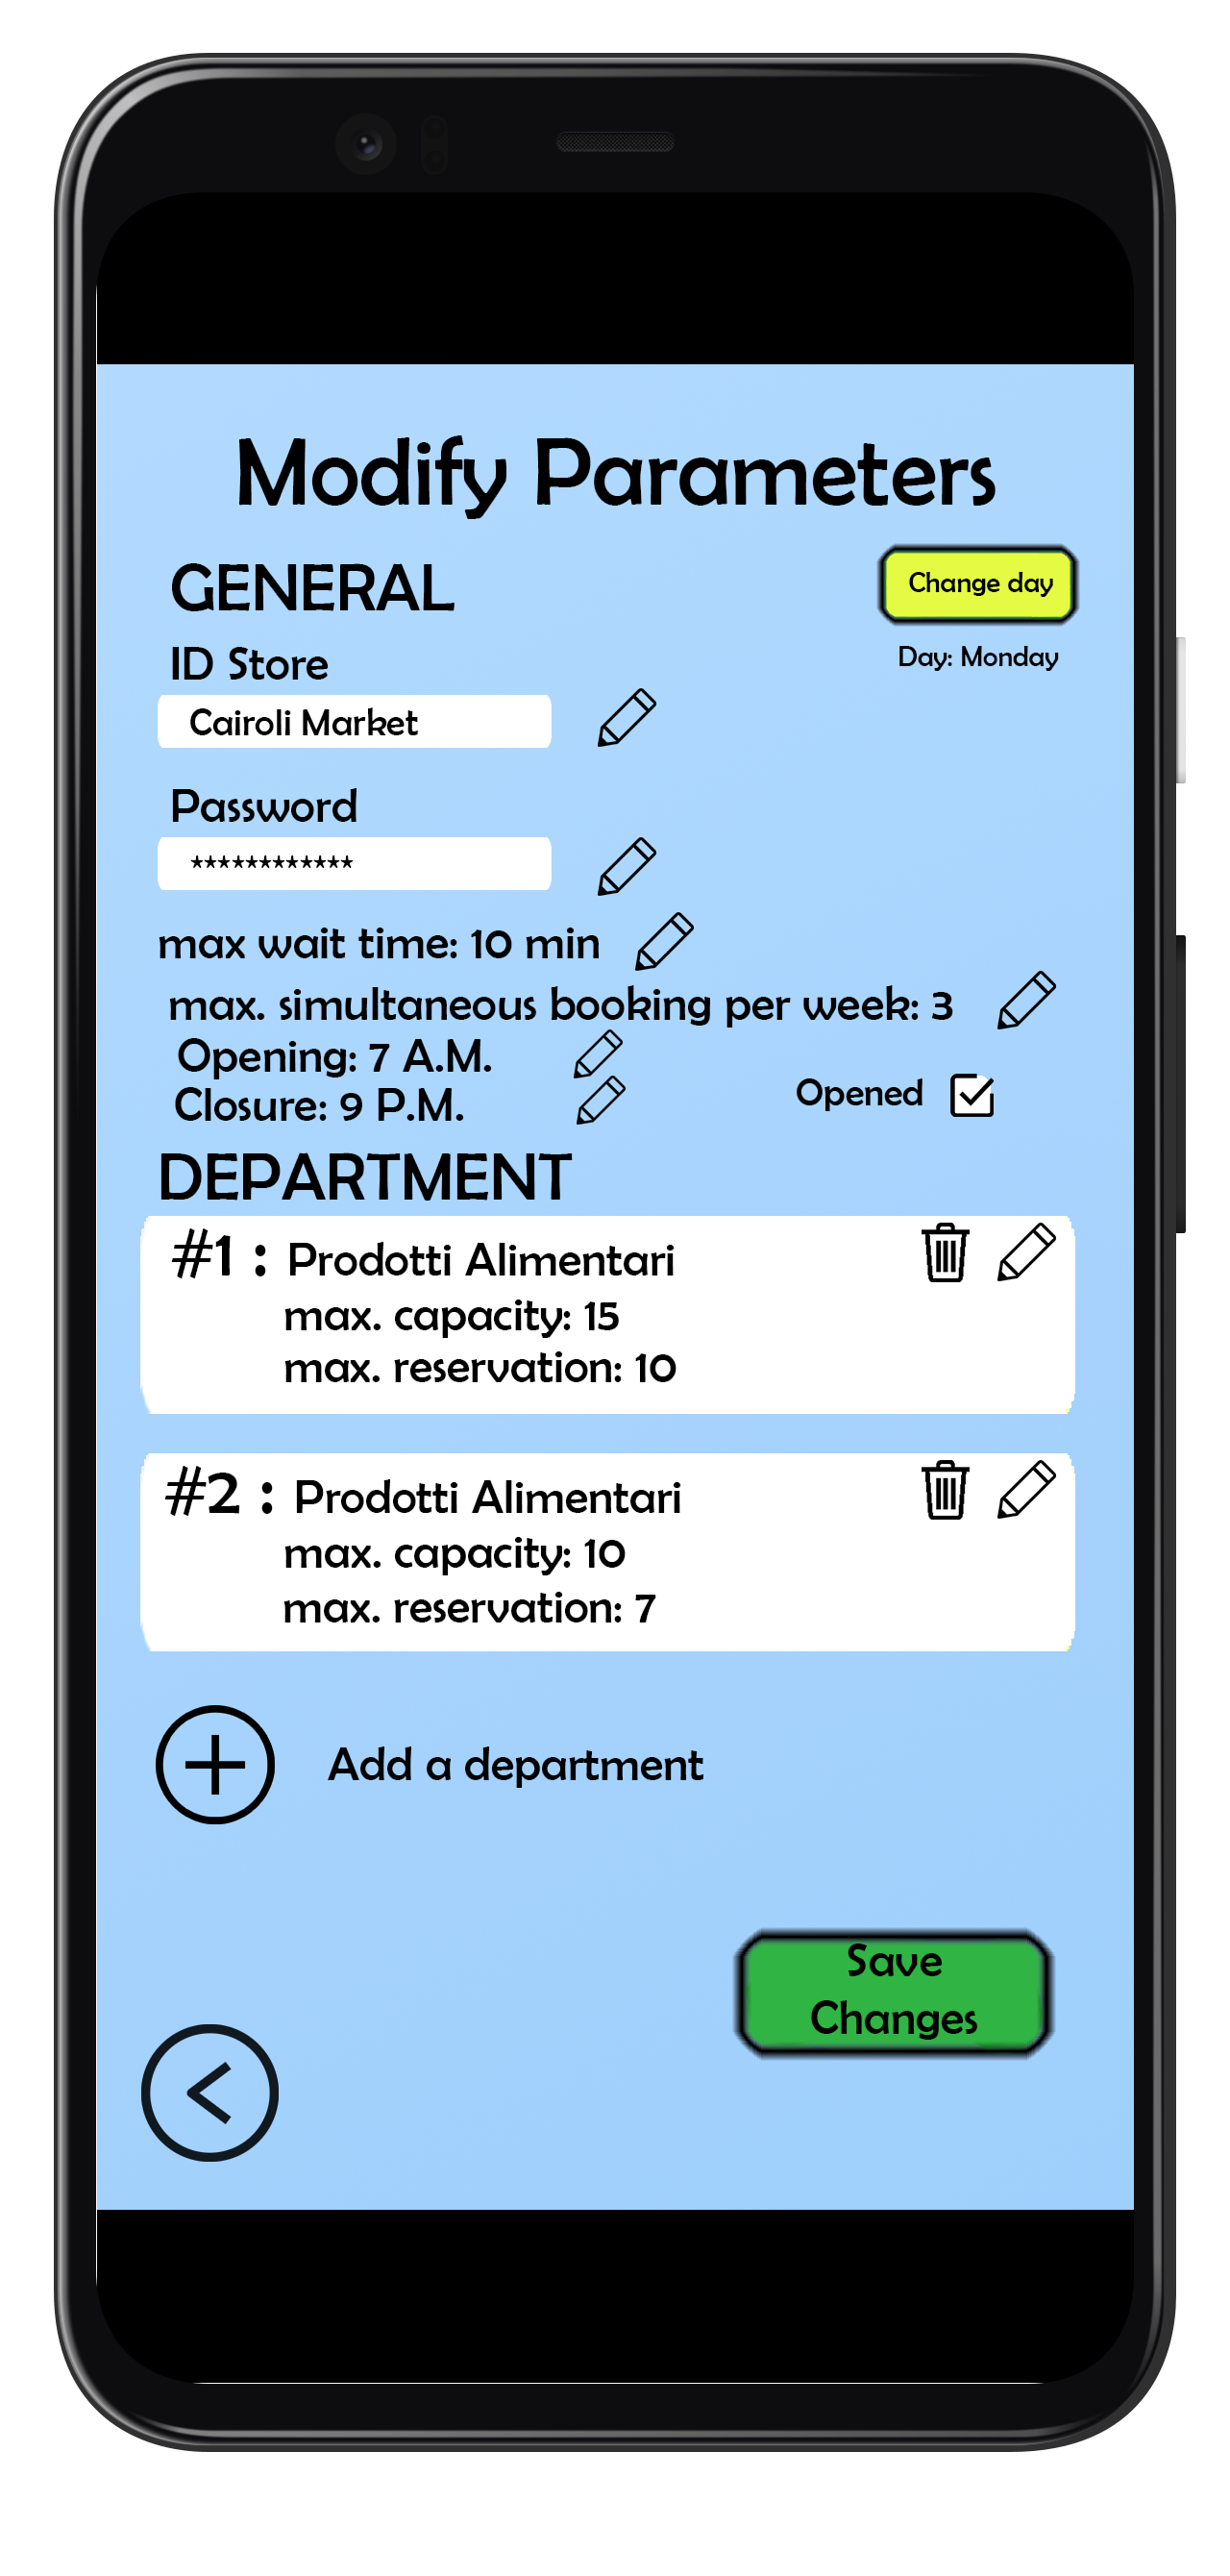
\includegraphics[width=\textwidth]{../Mockups/ModifyParameters.png}
			\caption{\emph{Modify store parameters}}
		\end{minipage}
	\end{figure}
			
			
		\subsubsection{Hardware Interfaces}
		
			The managers’ side of the application doesn’t require any special hardware requirement except for a network module installed in their device, since all of the information required are already in the system. Clients’ devices, anyway, require a working \emph{GPS} module, a working network module and a not broken display to scan the generated \emph{QR Code} at the store entry. Instead, at the store are needed a device with a ticket printer and a working network module to generate and print tickets, some (at least one for entry and one for exit) optical scanners to scan \emph{QR Codes} and another device with a working network module to manage ticket calling.
			
			
		\subsubsection{Software Interfaces}
		
			The system can send notification to the customer with regard to notify him to depart in time for reach the store and to avoid losing his turn in lineup. To do this, the system uses a public \emph{API} to get customer exact position by his \emph{GPS} module and, so, calculate the optimal route from customer's position to the store. The exact position is also used to sort by distance the list of bookable store. Since the alert is sent by a notification, the system use the \emph{API} of a notification service to provide notifications to customers. Moreover, notifications are used when the store manager modifies customers' reservations. Instead, the system uses the \emph{API} of a mail service when a store manager contacts some client.
			
		\subsubsection{Communication Interfaces}
		
			It is necessary to develop a communication interface in order to allow the different systems to communicate one to each other, achieving the integration of the store’s side and of the user’s side.
	\newpage
	\subsection{Functional Requirements}
	
		\subsubsection{List of Requirements}
		
			\begin{center}
				
				\rowcolors{2}{}{gray!20}
				\rowcolors{1}{gray!20}{white}
				\renewcommand{\arraystretch}{2}
				
				\setlength\LTleft{-2.4cm}
				\begin{longtable}[h!]{|m{2.5em}|m{37.5em}|}
						
					\hline
					\xrowht{5pt}
					\centering R1 & The system must allow the customers to register \\
					\xrowht{5pt}
					\centering R2 & The system must allow store managers to register their store \\
					\xrowht{5pt}
					\centering R3 & The system must allow customers to log in \\
					\xrowht{5pt}
					\centering R4 & The system must allow store managers to log in \\
					\xrowht{5pt}
					\centering R5 & The system allows the customers to view their visits \\
					\xrowht{5pt}
					\centering R6 & The system allows the customers to cancel their visits \\
					\xrowht{5pt}
					\centering R7 & The system allows the customers to modify their visits \\
					\xrowht{5pt}
					\centering R8 & The system allows the customers to select their favourite means of transportation \\
					\xrowht{5pt}
					\centering R9 & The system allows customers to select the departments in which they are interested in doing shopping \\
					\xrowht{5pt}
					\centering R10 & The system must let in customers only if it's their turn \\
					\xrowht{5pt}
					\centering R11 & The system must consider the estimate shopping time inserted by customers \\
					\xrowht{5pt}
					\centering R12 & The system must show the customers of the time periods in which they can enter the store, accordingly to the estimate of customers' shopping time \\
					\xrowht{5pt}
					\centering R13 & The system have to make a reasonable estimate of when a user with a spot on the queue is able to enter the store \\
					\xrowht{5pt}
					\centering R14 & The system can send notification to the clients \\
					\xrowht{5pt}
					\centering R15 & The system is able to ask for the position of the customers \\
					\xrowht{5pt}
					\centering R16 & The system permits to store manager to modify some critical parameters of the store related to customers' affluence management \\
					\xrowht{5pt}
					\centering R17 & The system allows the manager to establish the maximum simultaneously allowed booked clients in a specific department \\
					\xrowht{5pt}
					\centering R18 & The store manager can view the reservation of each client \\
					\hline
					\hline
					\xrowht{5pt}
					\centering R19 & The store manager can modify the reservation of each client \\
					\xrowht{5pt}
					\centering R20 & The store manager can cancel the reservation of each client \\
					\xrowht{5pt}
					\centering R21 & The store manager can handle the working days and hours of the store, for each day of the week \\
					\xrowht{5pt}
					\centering R22 & The system knows the situation in real time of each store \\
					\xrowht{5pt}
					\centering R23 & The system takes trace of each customer entry and exit from the store \\
					\xrowht{5pt}
					\centering R24 & The system contains a list of bookable stores \\
					\xrowht{5pt}
					\centering R25 & The system is able to print a paper ticket \\
					\xrowht{5pt}
					\centering R26 & The system can reasonably estimate the time needed from a customer to complete his shopping \\
					\xrowht{5pt}
					\centering R27 & The system saves clients' tickets \\
					\xrowht{5pt}
					\centering R28 & The system is able to smartly call clients with a ticket to enter the building depending on reservations and people inside the building \\
					\centering R29 & The system is able to scan and analyse a \emph{QR Code} \\
					\centering R30 & The system is able to send emails \\
					\centering R31 & The system knows how the maximum number of bookings allowed weekly per customer \\
					\centering R32 & The system can automatically rearrange reservations, if necessary \\
					\hline
					
				\end{longtable}
			\end{center}
		\newpage
		\subsubsection{Mapping with goals}
			
			\begin{itemize}			

				\item {\bfseries G1: Allow customers to select a store and book a visit on a certain date and time
				from\emph{CLup} app}			

					\begin{itemize}
						
						\item {\bfseries R1}: The system must allow the customers to register
						\item {\bfseries R2}: The system must allow customers to log in
						\item {\bfseries R9}: The system allows customers to select the departments in which they are interested in doing shopping						\item {\bfseries R11}: The system must consider the estimate shopping time inserted by customers
						\item {\bfseries R12}: The system must show the customers of the time periods in which they can enter the store, according to store's booking policies and the estimate of customers' shopping time
						\item {\bfseries R13}: The system have to make a reasonable estimate of when a user with a spot on the queue is able to enter the store
						\item {\bfseries R15}: The system is able to ask for the position of the customers
						\item {\bfseries R22}: The system knows the situation in real time of each store 
						\item {\bfseries R24}: The system contains a list of bookable stores
						\item {\bfseries R26}: The system can reasonably estimate the time needed from a customer to complete his shopping
						\item {\bfseries R27}: The system saves clients' tickets \\	
									
						\item {\bfseries DA1}: Date and time on the devices on which \emph{CLup} runs are always correct
						\item {\bfseries DA2}: Internet connection works always without errors
						\item {\bfseries DA3}: Customer’s position retrieved by \emph{GPS} is accurate
						\item {\bfseries DA8}: Every store has a unique name and address combination
						\item {\bfseries DA14}: The working days and hours of the store inserted in the system are corrected
					
					\end{itemize}
				
				\item {\bfseries G2: Allow customers to select a store and take a spot on the queue to enter as soon as possible the store from \emph{CLup} app}	

					\begin{itemize}
						
						\item {\bfseries R1}: The system must allow the customers to register
						\item {\bfseries R2}: The system must allow customers to log in
						\item {\bfseries R9}: The system allows customers to select the departments in which they are interested in doing shopping							\item {\bfseries R11}: The system must consider the estimate shopping time inserted by customers
						\item {\bfseries R15}: The system is able to ask for the position of the customers
						\item {\bfseries R22}: The system knows the situation in real time of each store
						\item {\bfseries R24}: The system contains a list of bookable stores
						\item {\bfseries R26}: The system can reasonably estimate the time needed from a customer to complete his shopping
						\item {\bfseries R27}: The system saves clients' tickets \\
		
						\item {\bfseries DA1}: Date and time on the devices on which \emph{CLup} runs are always correct
						\item {\bfseries DA2}: Internet connection works always without errors
						\item {\bfseries DA3}: Customer’s position retrieved by \emph{GPS} is accurate
						\item {\bfseries DA8}: Every store has a unique name and address combination
						\item {\bfseries DA14}: The working days and hours of the store inserted in the system are corrected
						
					\end{itemize}

				\item {\bfseries G3: Allow customers to take a spot on the queue from a physical ticket dispenser}	

					\begin{itemize}
						
						\item {\bfseries R9}: The system allows customers to select the departments in which they are interested in doing shopping
						\item {\bfseries R11}: The system must consider the estimate shopping time inserted by customers
						\item {\bfseries R13}: The system have to make a reasonable estimate of when a user with a spot on the queue is able to enter the store
						\item {\bfseries R25}: The system is able to print a paper ticket
						\item {\bfseries R26}: The system can reasonably estimate the time needed from a customer to complete his shopping
						\item {\bfseries R27}: The system saves clients' tickets \\
						
						\item {\bfseries DA1}: Date and time on the devices on which \emph{CLup} runs are always correct
						\item {\bfseries DA2}: Internet connection works always without errors
						\item {\bfseries DA5}: Totems always work properly and are not damaged
						\item {\bfseries DA14}: The working days and hours of the store inserted in the system are corrected
						
					\end{itemize}
				\newpage
				\item {\bfseries G4: Allow customers to have suggestions on better store options}	

					\begin{itemize}
						
						\item {\bfseries R1}: The system must allow the customers to register
						\item {\bfseries R2}: The system must allow customers to log in
						\item {\bfseries R8}: The system allows the customers to select their favourite means of transportation
						\item {\bfseries R11}: The system must consider the estimate shopping time inserted by customers
						\item{\bfseries R12:} The system must show the customers of the time periods in which they can enter the store, accordingly to the estimate of customers' shopping time
						\item {\bfseries R13}: The system have to make a reasonable estimate of when a user with a spot on the queue is able to enter the store
						\item {\bfseries R15}: The system is able to ask for the position of the customers
						\item {\bfseries R22}: The system knows the situation in real time of each store
						\item {\bfseries R24}: The system contains a list of bookable stores
						\item {\bfseries R26}: The system can reasonably estimate the time needed from a customer to complete his shopping	\\
		
						\item {\bfseries DA1}: Date and time on the devices on which \emph{CLup} runs are always correct
						\item {\bfseries DA2}: Internet connection works always without errors
						\item {\bfseries DA3}: Customer’s position retrieved by \emph{GPS} is accurate
						\item {\bfseries DA7}: The \emph{Maps API} always calculate the optimal route 
						\item {\bfseries DA8}: Every store has a unique name and address combination
						\item {\bfseries DA14}: The working days and hours of the store inserted in the system are corrected
						
					\end{itemize}

				\item {\bfseries G5: Allow customers to decrease waiting times specifying departments they want to visit}	

					\begin{itemize}
						
						\item {\bfseries R1}: The system must allow the customers to register
						\item {\bfseries R2}: The system must allow customers to log in
						\item {\bfseries R9}: The system allows customers to select the departments in which they are interested in doing shopping
						\item {\bfseries R11}: The system must consider the estimate shopping time inserted by customers
						\item {\bfseries R13}: The system have to make a reasonable estimate of when a user with a spot on the queue is able to enter the store
						\item {\bfseries R23}: The system takes trace of each customer entry and exit from the store
						\item {\bfseries R26}: The system can reasonably estimate the time needed from a customer to complete his shopping \\
						
						\item {\bfseries DA1}: Date and time on the devices on which \emph{CLup} runs are always correct
						\item {\bfseries DA2}: Internet connection works always without errors
						\item {\bfseries DA14}: The working days and hours of the store inserted in the system are corrected
						
					\end{itemize}

				\item {\bfseries G6: Allow customers users to manage their reservations}	

					\begin{itemize}
						\item {\bfseries R1}: The system must allow the customers to register
						\item {\bfseries R2}: The system must allow customers to log in
						\item {\bfseries R5}: The system allows the customers to view their visits
						\item {\bfseries R6}: The system allows the customers to cancel their visits
						\item {\bfseries R7}: The system allows the customers to modify their visits
						\item {\bfseries R27}: The system saves clients' tickets \\
		
						\item {\bfseries DA1}: Date and time on the devices on which \emph{CLup} runs are always correct
						\item {\bfseries DA2}: Internet connection works always without errors
							
					\end{itemize}

				 
				
				\item {\bfseries G7: Allow customers to depart from their location in time to avoid waiting too much, and to avoid losing their turn for entering}	

					\begin{itemize}
						\item {\bfseries R1}: The system must allow the customers to register
						\item {\bfseries R2}: The system must allow customers to log in
						\item {\bfseries R8}: The system allows the customers to select their favourite means of transportation
						\item {\bfseries R9}: The system allows customers to select the departments in which they are interested in doing shopping
						\item {\bfseries R11}: The system must consider the estimate shopping time inserted by customers
						\item {\bfseries R13}: The system have to make a reasonable estimate of when a user with a spot on the queue is able to enter the store
						\item {\bfseries R14}: The system can send notification to the clients
						\item {\bfseries R15}: The system is able to ask for the position of the customers
						\item {\bfseries R23}: The system takes trace of each customer entry and exit from the store
						\item {\bfseries R26}: The system can reasonably estimate the time needed from a customer to complete his shopping
						\item {\bfseries R27}: The system saves clients' tickets \\
					
						\item {\bfseries DA1}: Date and time on the devices on which \emph{CLup} runs are always correct
						\item {\bfseries DA2}: Internet connection works always without errors
						\item{\bfseries DA3}: Customer’s position retrieved by \emph{GPS} is accurate
						\item {\bfseries DA7}: The \emph{Maps API} always calculate the optimal route 
						\item {\bfseries DA8}: Every store has a unique name and address combination
						\item{\bfseries DA15}: All users are ready to depart for the store when they are notified
							
					\end{itemize}	


				\item {\bfseries G8: Allow the store manager to know the real situation of people that are inside the building and in which department of his store}	

					\begin{itemize}
						
						\item {\bfseries R2}: The system must allow store managers to register their store
						\item {\bfseries R4}: The system must allow store managers to log in
						\item {\bfseries R23}: The system takes trace of each customer entry and exit from the store
						\item {\bfseries R29}: The system is able to scan and analyse a \emph{QR Code} \\		
				
						\item {\bfseries DA1}: Date and time on the devices on which \emph{CLup} runs are always correct
						\item {\bfseries DA2}: Internet connection works always without errors
						\item {\bfseries DA9}: \emph{QR Code} readers are always working
						\item {\bfseries DA12}: Each customer scans his \emph{QR Code} at the enter and enters the supermarket only through the allowed entries.
							
					\end{itemize}

				\item {\bfseries G9: Allow to grant a fair management of users that can access the building.}	

					\begin{itemize}
						
						\item {\bfseries R2}: The system must allow store managers to register their store
						\item {\bfseries R4}: The system must allow store managers to log in
						\item {\bfseries R10}: The system must let in customers only if it's their turn
						\item {\bfseries R17}: The system allows the manager to establish the maximum simultaneously allowed booked clients in a specific department
						\item {\bfseries R21}: The store manager can handle the working days and hours of the store, for each day of the week
						 
						\item {\bfseries R31}: The system knows how the maximum number of bookings allowed weekly per customer\\
						
						\item {\bfseries DA1}: Date and time on the devices on which \emph{CLup} runs are always correct
						\item {\bfseries DA2}: Internet connection works always without errors
						\item{\bfseries DA11}: Customer tries to respect their estimate, without remaining over time
					
					\end{itemize}
				
				\item {\bfseries G10: Allow to manage optimally the influx in the building and avoid gathering inside it}	

					\begin{itemize}
						\item {\bfseries R2}: The system must allow store managers to register their store
						\item {\bfseries R4}: The system must allow store managers to log in
											
						\item {\bfseries R10}: The system must let in customers only if it's their turn
						\item {\bfseries R16}: The system permits to store manager to modify some critical parameters of the store related to customers' affluence management
						\item {\bfseries R23}: The system takes trace of each customer entry and exit from the store
						\item {\bfseries R26}: The system saves clients' tickets				
						\item {\bfseries R28}: The system is able to smartly call clients with a ticket to enter the building depending on reservations and people inside the building
						\item {\bfseries R29}: The system is able to scan and analyse a \emph{QR Code}
						\item{\bfseries R32}: The system can automatically rearrange reservations, if necessary \\
		
						\item {\bfseries DA1}: Date and time on the devices on which \emph{CLup} runs are always correct
						\item {\bfseries DA2}: Internet connection works always without errors
						\item {\bfseries DA9}: \emph{QR Code} readers are always working
						\item{\bfseries DA6}: The customer’s smartphone screen is not damaged and the \emph{QR Code} is readable
						\item {\bfseries DA12}: Each customer scans his \emph{QR Code} at the enter and enters the supermarket only through the allowed entries
						\item {\bfseries DA13}: Each paper ticket is not ruined and readable
						\item {\bfseries DA14}: The working days and hours of the store inserted in the system are corrected
					
					\end{itemize}
				\newpage
				\item {\bfseries G11: Allow the store manager to interact with customers and reservations}	

					\begin{itemize}
						\item {\bfseries R2}: The system must allow store managers to register their store
						\item {\bfseries R4}: The system must allow store managers to log in
						\item {\bfseries R14}: The system can send notification to the clients
						\item {\bfseries R18}: The store manager can cancel the reservation of each client
						\item {\bfseries R19}: The store manager can modify the reservation of each client
						\item {\bfseries R20}: The store manager can view the reservation of each client
						\item {\bfseries R26}: The system saves clients' tickets
						\item{\bfseries R30}: The system is able to send emails \\
		
						\item {\bfseries DA1}: Date and time on the devices on which \emph{CLup} runs are always correct
						\item {\bfseries DA2}: Internet connection works always without errors
						\newpage
		
					\end{itemize}

			\end{itemize}

		\subsubsection{Use Cases}
		

			
			\paragraph{Registration of a customer}
			
				\begin{center}
					
					\rowcolors{2}{}{gray!20}
					\rowcolors{1}{gray!20}{white}
					
					\begin{adjustwidth}{-3cm}{}
					\begin{tabular}[h!]{|m{7.5em}|m{36em}|}
						
						\hline
						\xrowht{5pt}
						Name &  Registration of a customer\\
						\xrowht{5pt}
						Actors & Customer\\
						\xrowht{5pt}
						Entry Condition & Customer has the internet connection available and has accessed on the application on its device\\
						\xrowht{5pt}
						Event Flow & \begin{enumerate}
							
							\itemsep-0.25em
							\item Customer visualizes the initial page of the app
							\item Customer clicks on “Sign up as customer” button
							\item Customer inserts a username, a password, an e-mail, his name, his surname and his phone number as mandatory fields
							\item The system checks the data of the customer
							\item The system saves the information of the customer
						
						\end{enumerate}\\
						\xrowht{5pt}
						Exit Conditions & Customer is successfully registered to the application\\
						\xrowht{5pt}
						Exception & \begin{enumerate}
							
							\itemsep-0.25em
							\item The username is already present in the system
							\item The customer did not fill up all the mandatory fields with valid data
						
						\end{enumerate}
						If one or more of the above situations occur, the application will throw an error message and will return to the registration form page\\		
						\hline
						
					\end{tabular}

					
					

					\begin{figure}[!h]
						\begin{adjustwidth} {-0.8cm}{}
							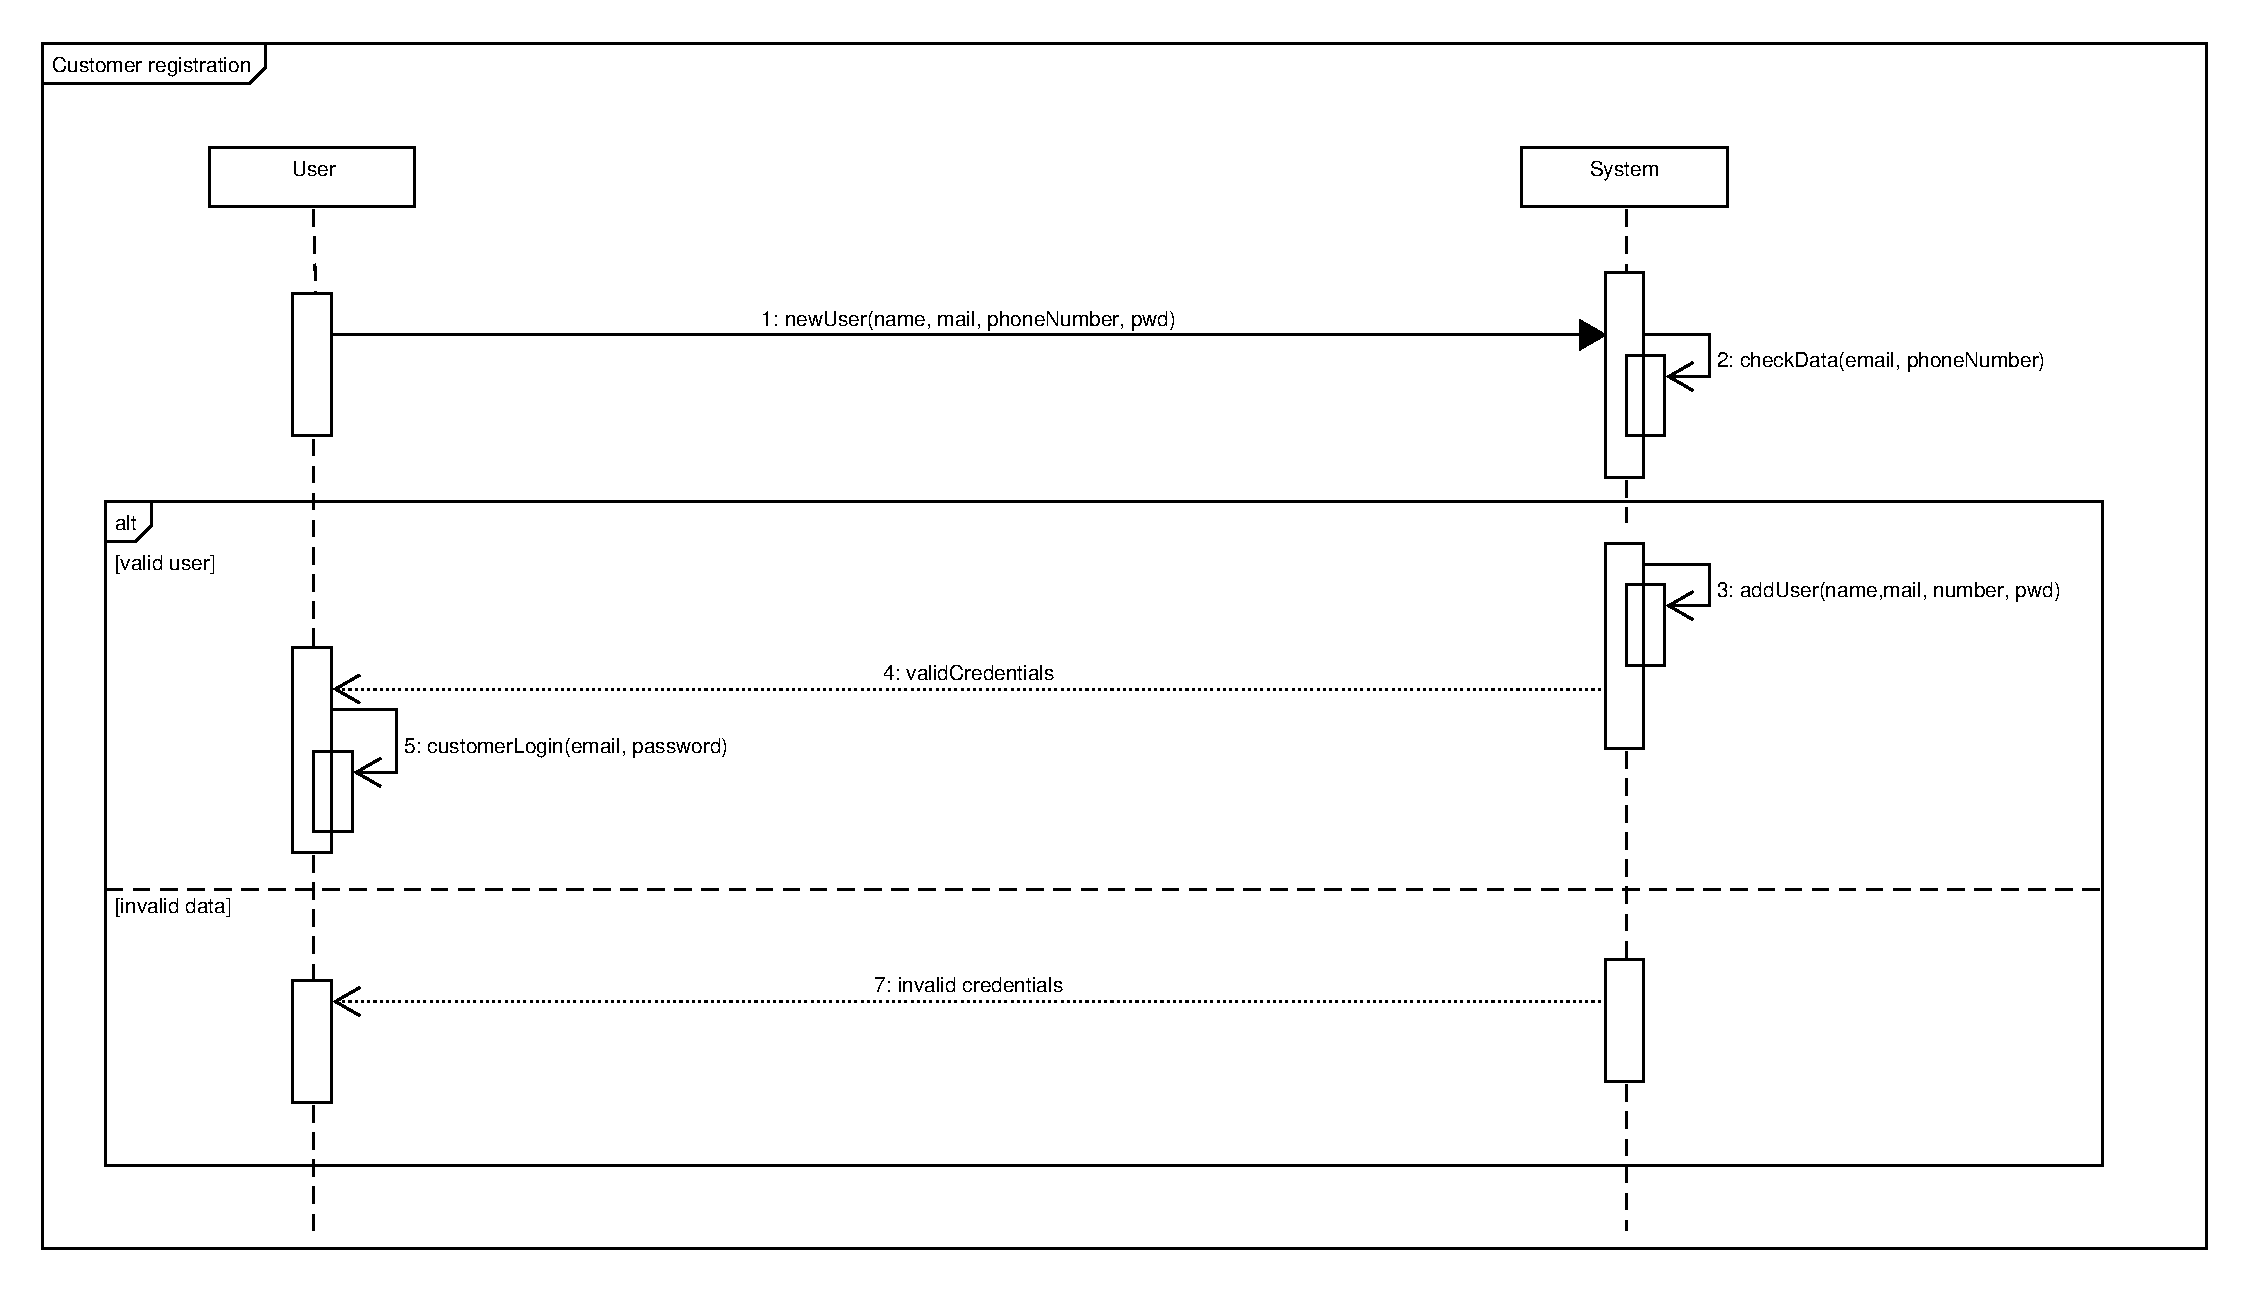
\includegraphics[scale=0.36]{SD/1_customerRegistration.pdf}
						\end{adjustwidth}
						\caption{\emph{Sequence Diagram of Customer Registration}}
					\end{figure}
					\end{adjustwidth}
				
					\begin{itemize}
					\medskip
					{\bfseries Required functional requirements: }
					\item {\bfseries R1}: The system must allow the customers to register


					\end{itemize}
				\end{center}
			\bigskip
			\paragraph{Registration of a store}
			
				\begin{center}
					
					\rowcolors{2}{}{gray!20}
					\rowcolors{1}{gray!20}{white}
					
					\begin{adjustwidth}{-3cm}{}
					\begin{tabular}[h!]{|m{7.5em}|m{36em}|}
						
						\hline
						\xrowht{5pt}
						Name & Registration of a store\\
						\xrowht{5pt}
						Actors & Store manager\\
						\xrowht{5pt}
						Entry Condition & Store manager has the internet connection available and has accessed the application on its device\\
						\xrowht{5pt}
						Event Flow & \begin{enumerate}
							
							\itemsep-0.25em
							\item Store manager visualizes the initial page of the app
							\item Store manager clicks on “Sign up as store” button
							\item Store manager compile all the mandatory fields concerning the store
							\item Store manager loads a certification document which proves that it is a real store
							\item The system validates the certification
							\item The system confirms the registration of the store
							\item The system saves the information of the store
							
						\end{enumerate}\\
						\xrowht{5pt}
						Exit Conditions & The store is successfully registered to the application\\
						\xrowht{5pt}
						Exception & \begin{enumerate}
							
							\itemsep-0.25em
							\item The store is already present in the system
							\item The store manager did not fill up all the mandatory fields with valid data
							\item The certification is invalid
							
						\end{enumerate}
						If one or more of the above situations occur, the application will throw an error message and will return to the registration form page\\		
						\hline
						
					\end{tabular}
					\end{adjustwidth}
					
					\begin{itemize}
					\bigskip
					\bigskip
					\bigskip
					 {\bfseries Required functional requirements: }
					\item {\bfseries R2}: The system must allow store managers to register their store

					\end{itemize}
				
							\begin{figure}
								\begin{adjustwidth} {-2.5cm}{}
									\centering
									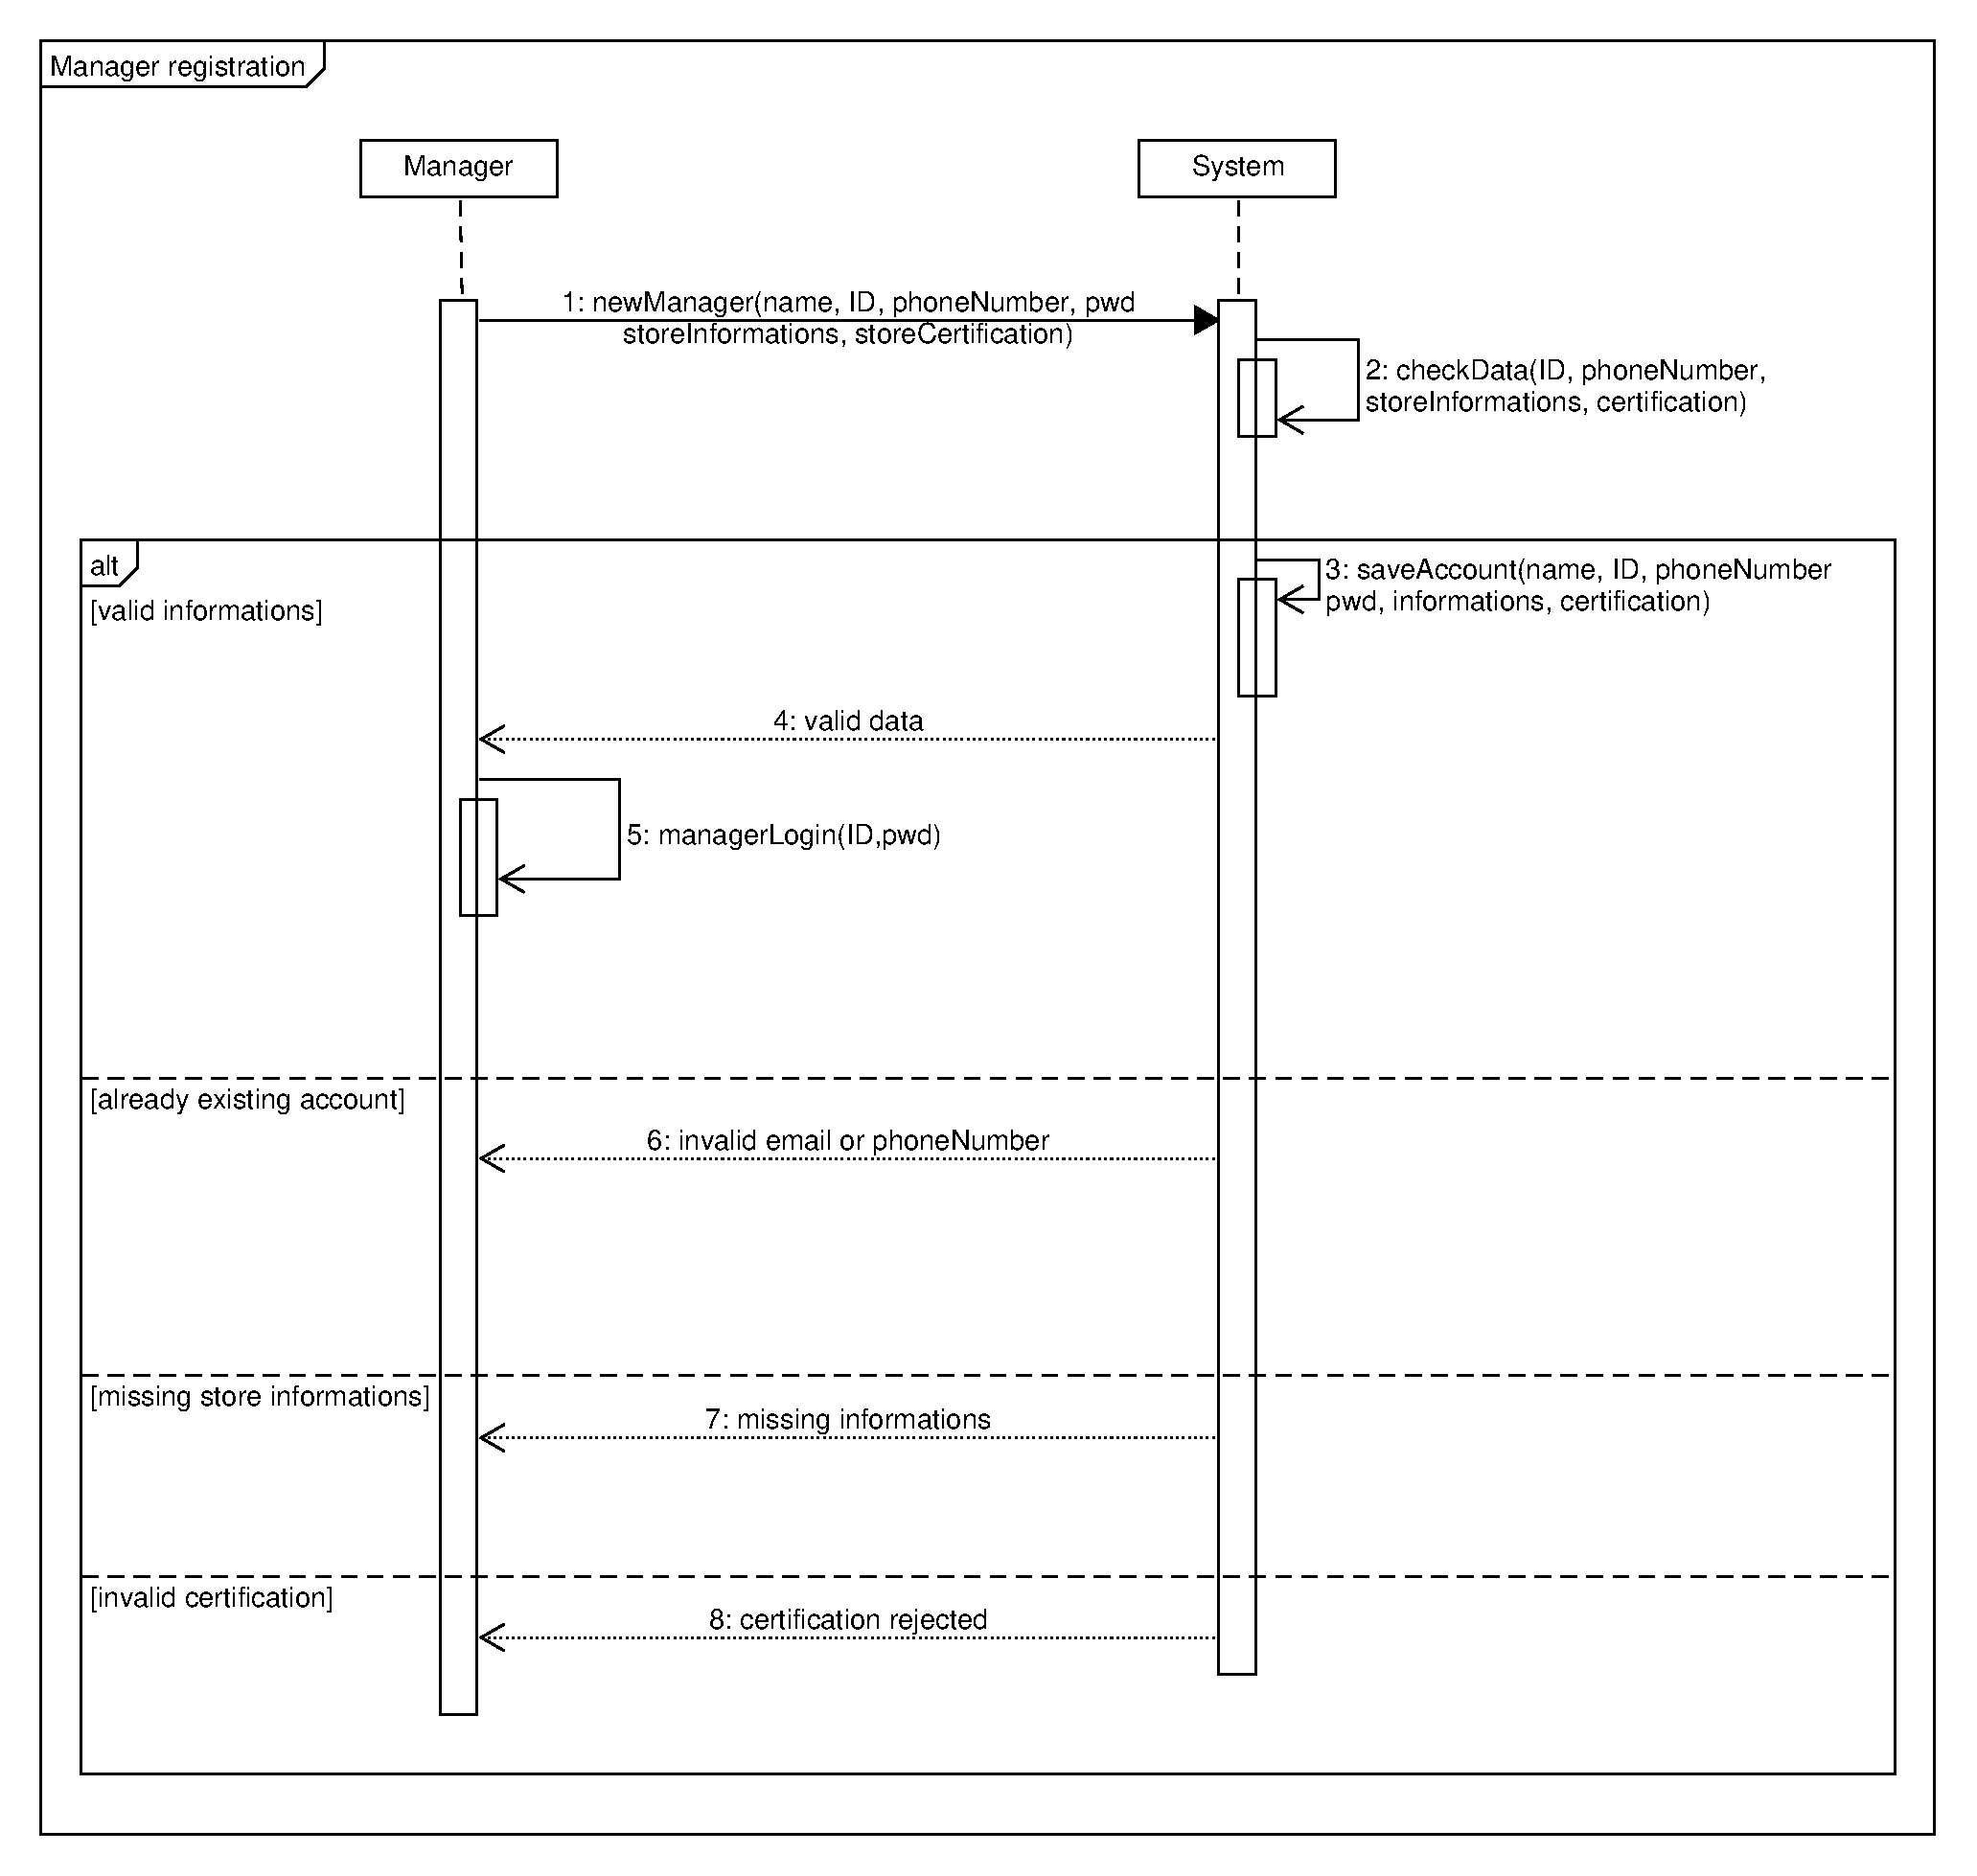
\includegraphics[scale=0.5]{SD/2_storeManagerRegistration.pdf}\\
									\caption{\emph{Sequence Diagram of Store Manager Registration}}
								\end{adjustwidth}
							\end{figure}

				\end{center}

			\newpage
			
			\paragraph{Login of a customer}
			
				\begin{center}
					
					\rowcolors{2}{}{gray!20}
					\rowcolors{1}{gray!20}{white}
					
					\begin{adjustwidth}{-3cm}{}
					\begin{tabular}[h!]{|m{7.5em}|m{36em}|}
						
						\hline
						\xrowht{5pt}
						Name & Login of a customer\\
						\xrowht{5pt}
						Actors & Customer\\
						\xrowht{5pt}
						Entry Condition & Customer is already registered to the application service\\
						\xrowht{5pt}
						Event Flow & \begin{enumerate}
							
							\itemsep-0.25em
							\item Customer accesses the application through its device
							\item Customer clicks on “Login as customer” button
							\item The system opens the “Login as customer” page
							\item Customer compiles the fields “Username” and “Password”
							\item Customer clicks on “Login” button
							\item The system opens the “Customer menu” page
							
						\end{enumerate}\\
						\xrowht{5pt}
						Exit Conditions & Customer has successfully logged in\\
						\xrowht{5pt}
						Exception & \begin{enumerate}
							
							\itemsep0em
							\item Customer enters invalid email
							\item Customer enters invalid password
							
						\end{enumerate}
						If one or more of the above situations occur, the application will throw an error message and will return to the “Login as customer” page\\		
						\hline
						
					\end{tabular}
					\end{adjustwidth}
					
					\begin{figure}[!h]
						\begin{adjustwidth} {-1.3cm}{}
							\centering
							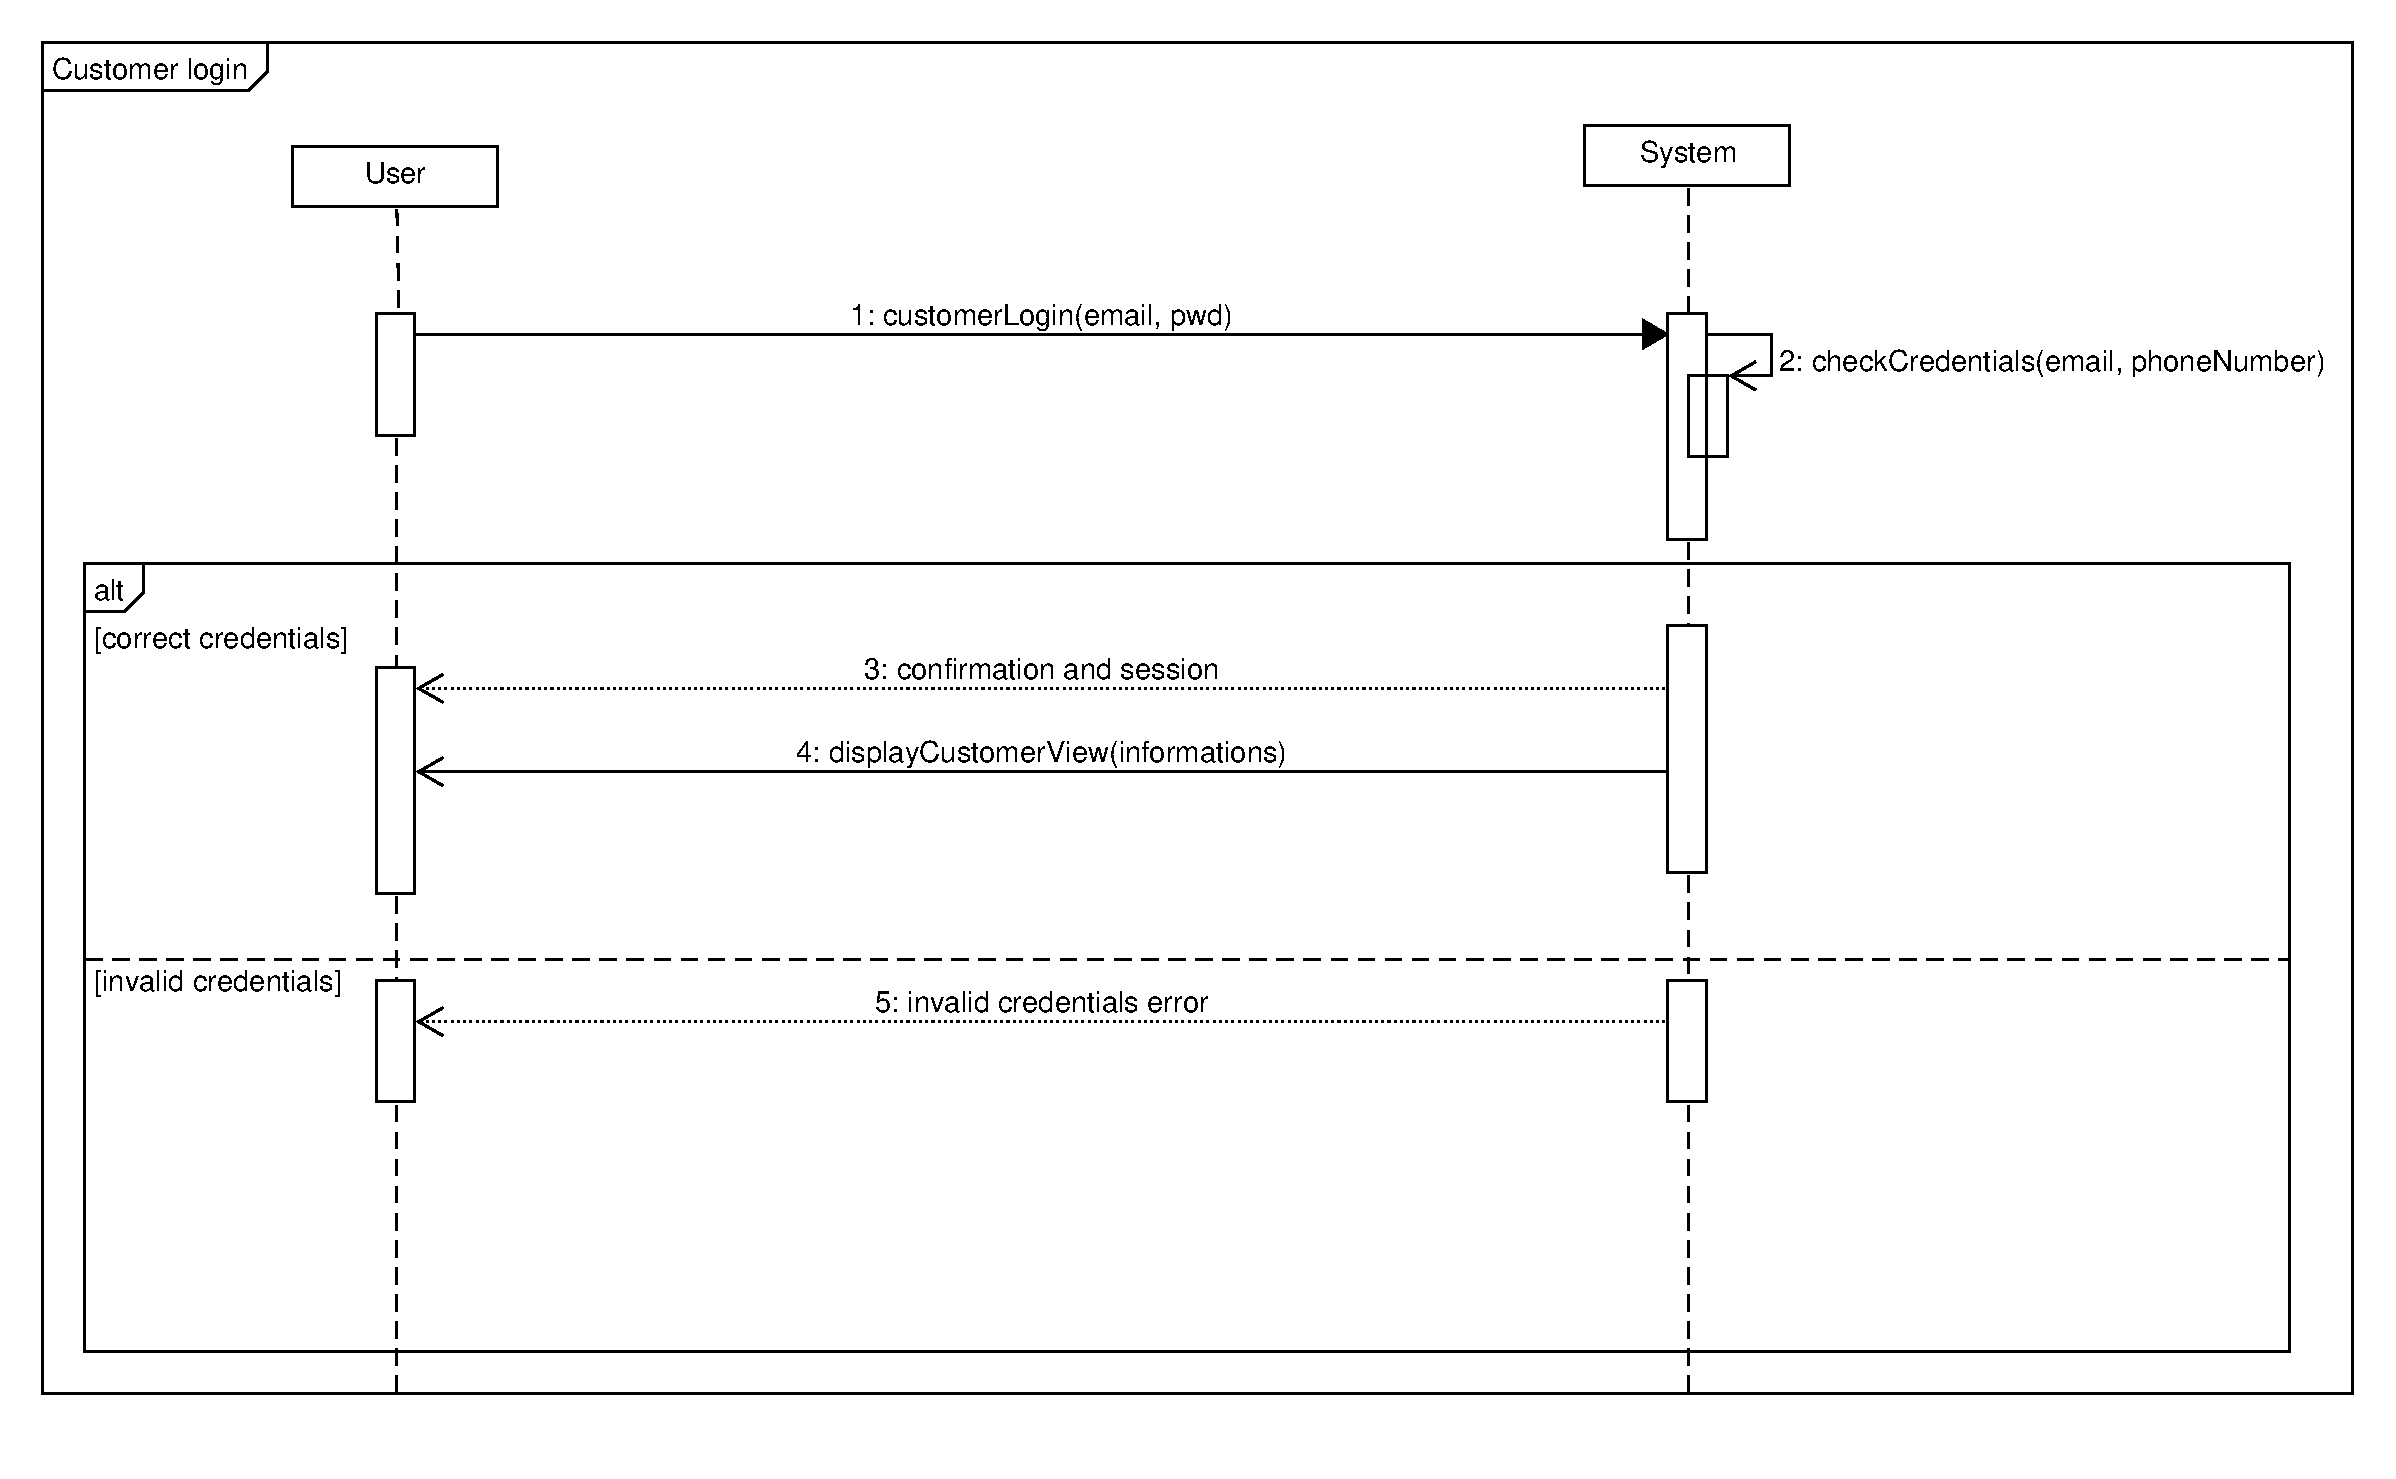
\includegraphics[scale=0.36]{SD/3_customerLogin.pdf}\\
							\caption{\emph{Sequence Diagram of Customer Login}}
						\end{adjustwidth}
					\end{figure}

					\begin{itemize}
					\bigskip
					\bigskip
					\bigskip
					 {\bfseries Required functional requirements: }
					\item {\bfseries R3}: The system must allow customers to log in

					\end{itemize}

				\end{center}
			
					\bigskip
					\bigskip
					\bigskip
			\paragraph{Login of a store manager}
			
				\begin{center}
					
					\rowcolors{2}{}{gray!20}
					\rowcolors{1}{gray!20}{white}
					
					\begin{adjustwidth}{-3cm}{}
					\begin{tabular}[h!]{|m{7.5em}|m{36em}|}
						
						\hline
						\xrowht{5pt}
						Name & Login of a store manager\\
						\xrowht{5pt}
						Actors & Store manager\\
						\xrowht{5pt}
						Entry Condition & Store manager’s store is already registered to the application service\\
						\xrowht{5pt}
						Event Flow & \begin{enumerate}
							
							\itemsep-0.25em
							\item Store manager accesses the application through its device
							\item Store manager clicks on “Login as store” button
							\item The system opens the “Login as store” page
							\item Store manager compiles the fields “ID” and “Password”
							\item Store manager clicks on “Login” button
							\item The system opens the “Store menu” page
							
						\end{enumerate}\\
						\xrowht{5pt}
						Exit Conditions & Store manager has successfully logged in\\
						\xrowht{5pt}
						Exception & \begin{enumerate}
							
							\itemsep-0.25em
							\item Store manager enters invalid ID
							\item Store manager enters invalid Password
							
						\end{enumerate}
						If one or more of the above situations occur, the application will throw an error message and will return to the “Login as store” page\\		
						\hline
						
					\end{tabular}
					\end{adjustwidth}

					\begin{itemize}
					\bigskip
					\bigskip
					\bigskip
					 {\bfseries Required functional requirements: }
					\item {\bfseries R4: } The system must allow store managers to log in
					

					\end{itemize}

							\begin{figure}
								\begin{adjustwidth} {-3cm}{}
									\centering
									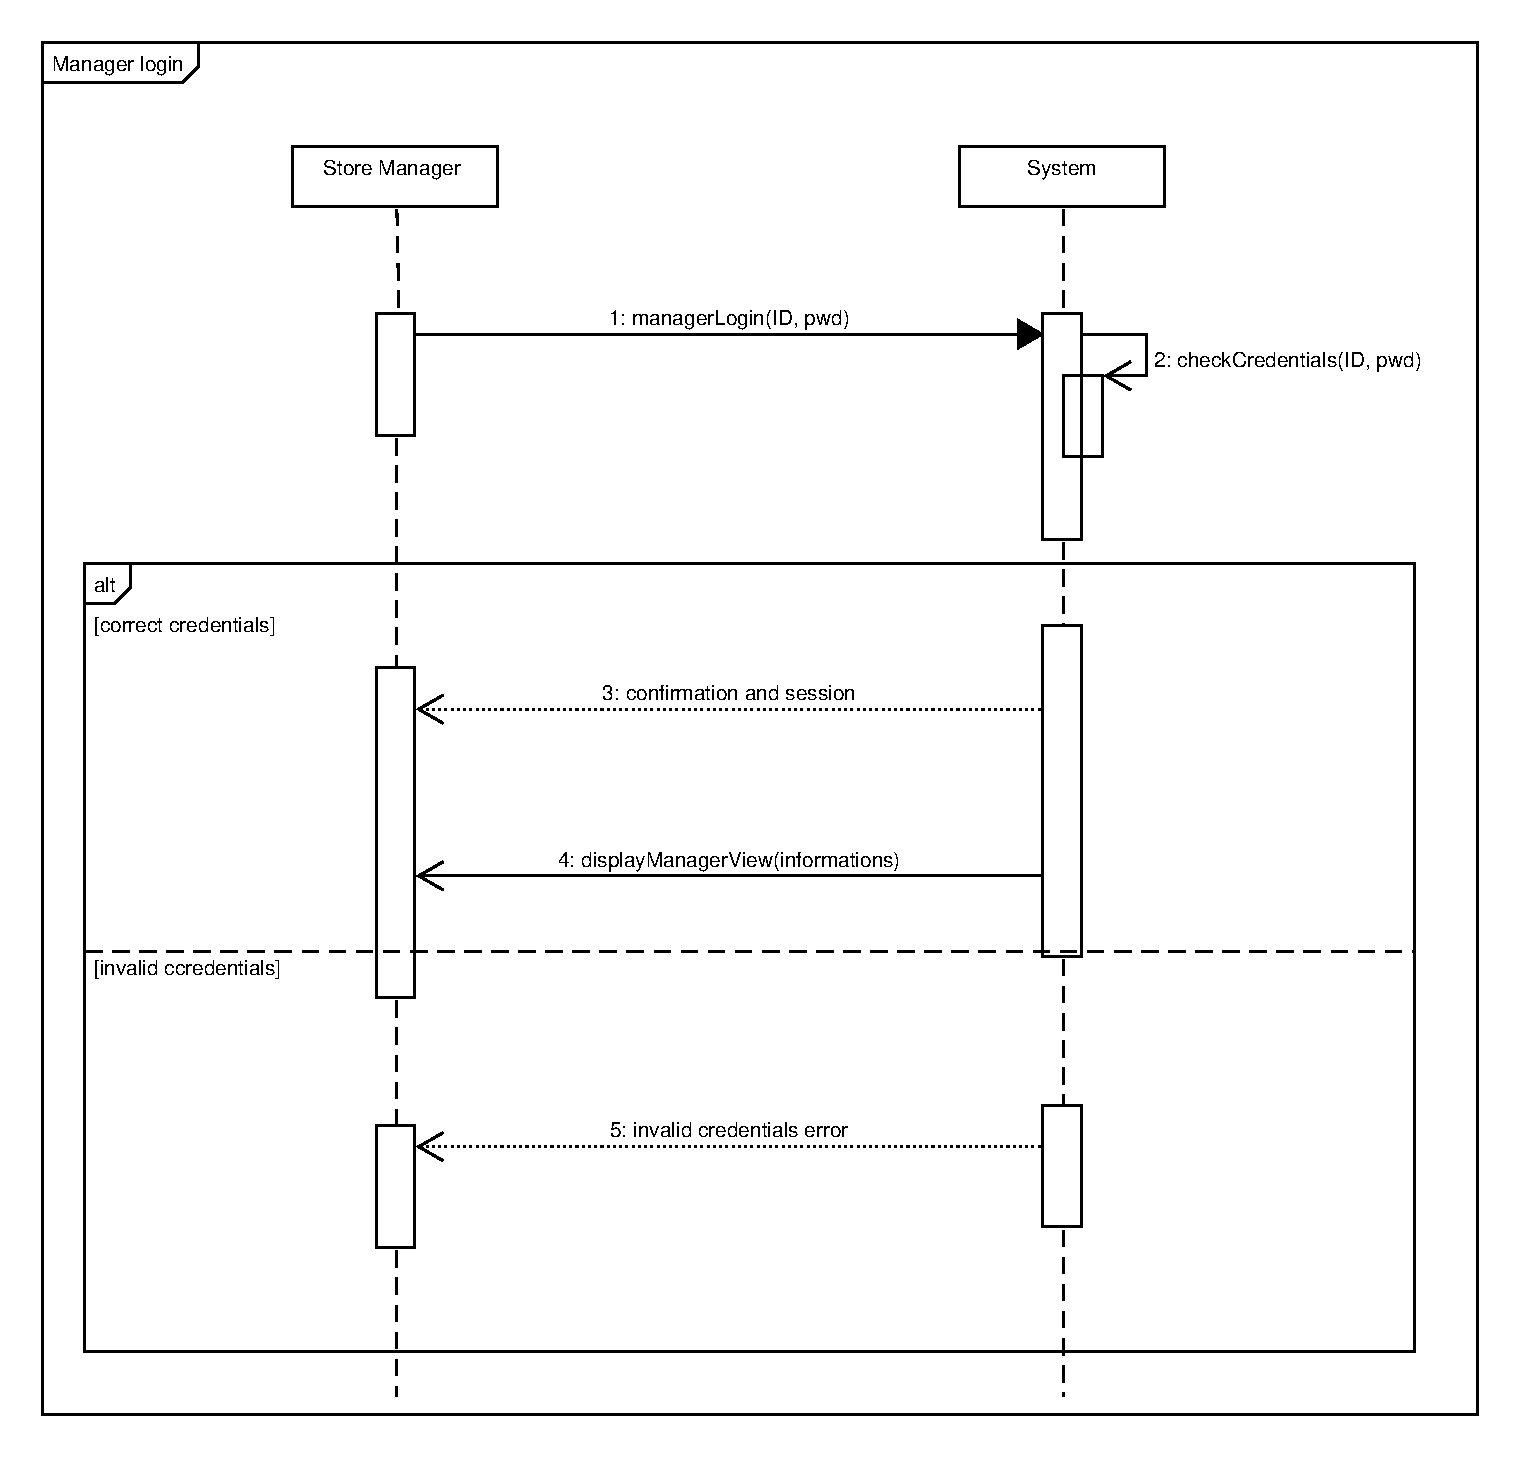
\includegraphics[scale=0.7]{SD/4_managerLogin.pdf}\\
									\caption{\emph{Sequence Diagram of Store Manager Login}}
								\end{adjustwidth}
							\end{figure}
					
				\end{center}
				\newpage
			
			\paragraph{Customer makes a reservation}
			
				\begin{center}
					
					\rowcolors{2}{}{gray!20}
					\rowcolors{1}{gray!20}{white}
					
					\begin{adjustwidth}{-3cm}{}
					\begin{tabular}[h!]{|m{7.5em}|m{36em}|}
						
						\hline
						\xrowht{5pt}
						Name & Customer makes a reservation\\
						\xrowht{5pt}
						Actors & Customer\\
						\xrowht{5pt}
						Entry Condition & Customer is already logged in the application service\\
						\xrowht{5pt}
						Event Flow & \begin{enumerate}
							
							\itemsep-0.25em
							\item Customer clicks on “Make a reservation”
							\item The customer can see the list of stores in his city and can filter this list by choosing a specific chain from a drop down menu, selects a store and clicks on Next
							\item Customer can see the list of all possible objects’ category and can select some of them (optional), and then clicks on Next
							\item Customer can estimate a duration for his shopping, or let the system to do it, and then clicks on Next
							\item Customer can see two button, “As soon as possible” and “Choose a time slot”
							 
							\begin{enumerate}
								
								\itemsep-0.25em
								\item if the clicks on “As soon as possible” button, the system will check that the customer isn't already on the queue, and will calculate the waiting time to enter. If a ticket with low waiting time is issuable, the system will generate it, saves it on both itself and user's app, showing it on the latter.
									 Otherwise, the system suggests him other options, included the previously selected store. If any good, customer accepts one of the suggested store and gets the reservation, otherwise cancel the procedure.
									 \medskip	

								
								\item if the customer clicks on “Book”, the user can choose a time to enter the store among the time intervals available on the “Time slots” page to generate and save the reservation. If the customer is not satisfied with the proposed options, can click on the "Suggestion" button, and the system will retrieve him other stores, where he can book with the selected preferences. Selecting the store, the "Time slots" page updates with the new store's options. When the customer is satisfied with the selection, clicks on the Book button and the system will issue the reservation.
								
							\end{enumerate}
							
						\end{enumerate}\\
						\xrowht{5pt}
						Exit Conditions & Customer has successfully made a reservation\\
						\xrowht{5pt}
						Exception & \begin{enumerate}
							
							\itemsep-0.25em
							\item Customer click on a timeslot no longer available or tries to book more than the set limit of reservations per week
							
							The application will throw an error message and will reload the “Time slots” page (updating it)
							\medskip
							\item In the selected store where get a spot on the queue there isn't availability in the day, and there isn't any available near store 

							If the above situation occurs, the application will throw an error and leave the client the possibility to book his visit.
							
							
						\end{enumerate}
							\\
							\hline
						
						
					\end{tabular}
					\end{adjustwidth}
					
							\begin{figure}
								\begin{adjustwidth} {0cm}{}
									\centering
									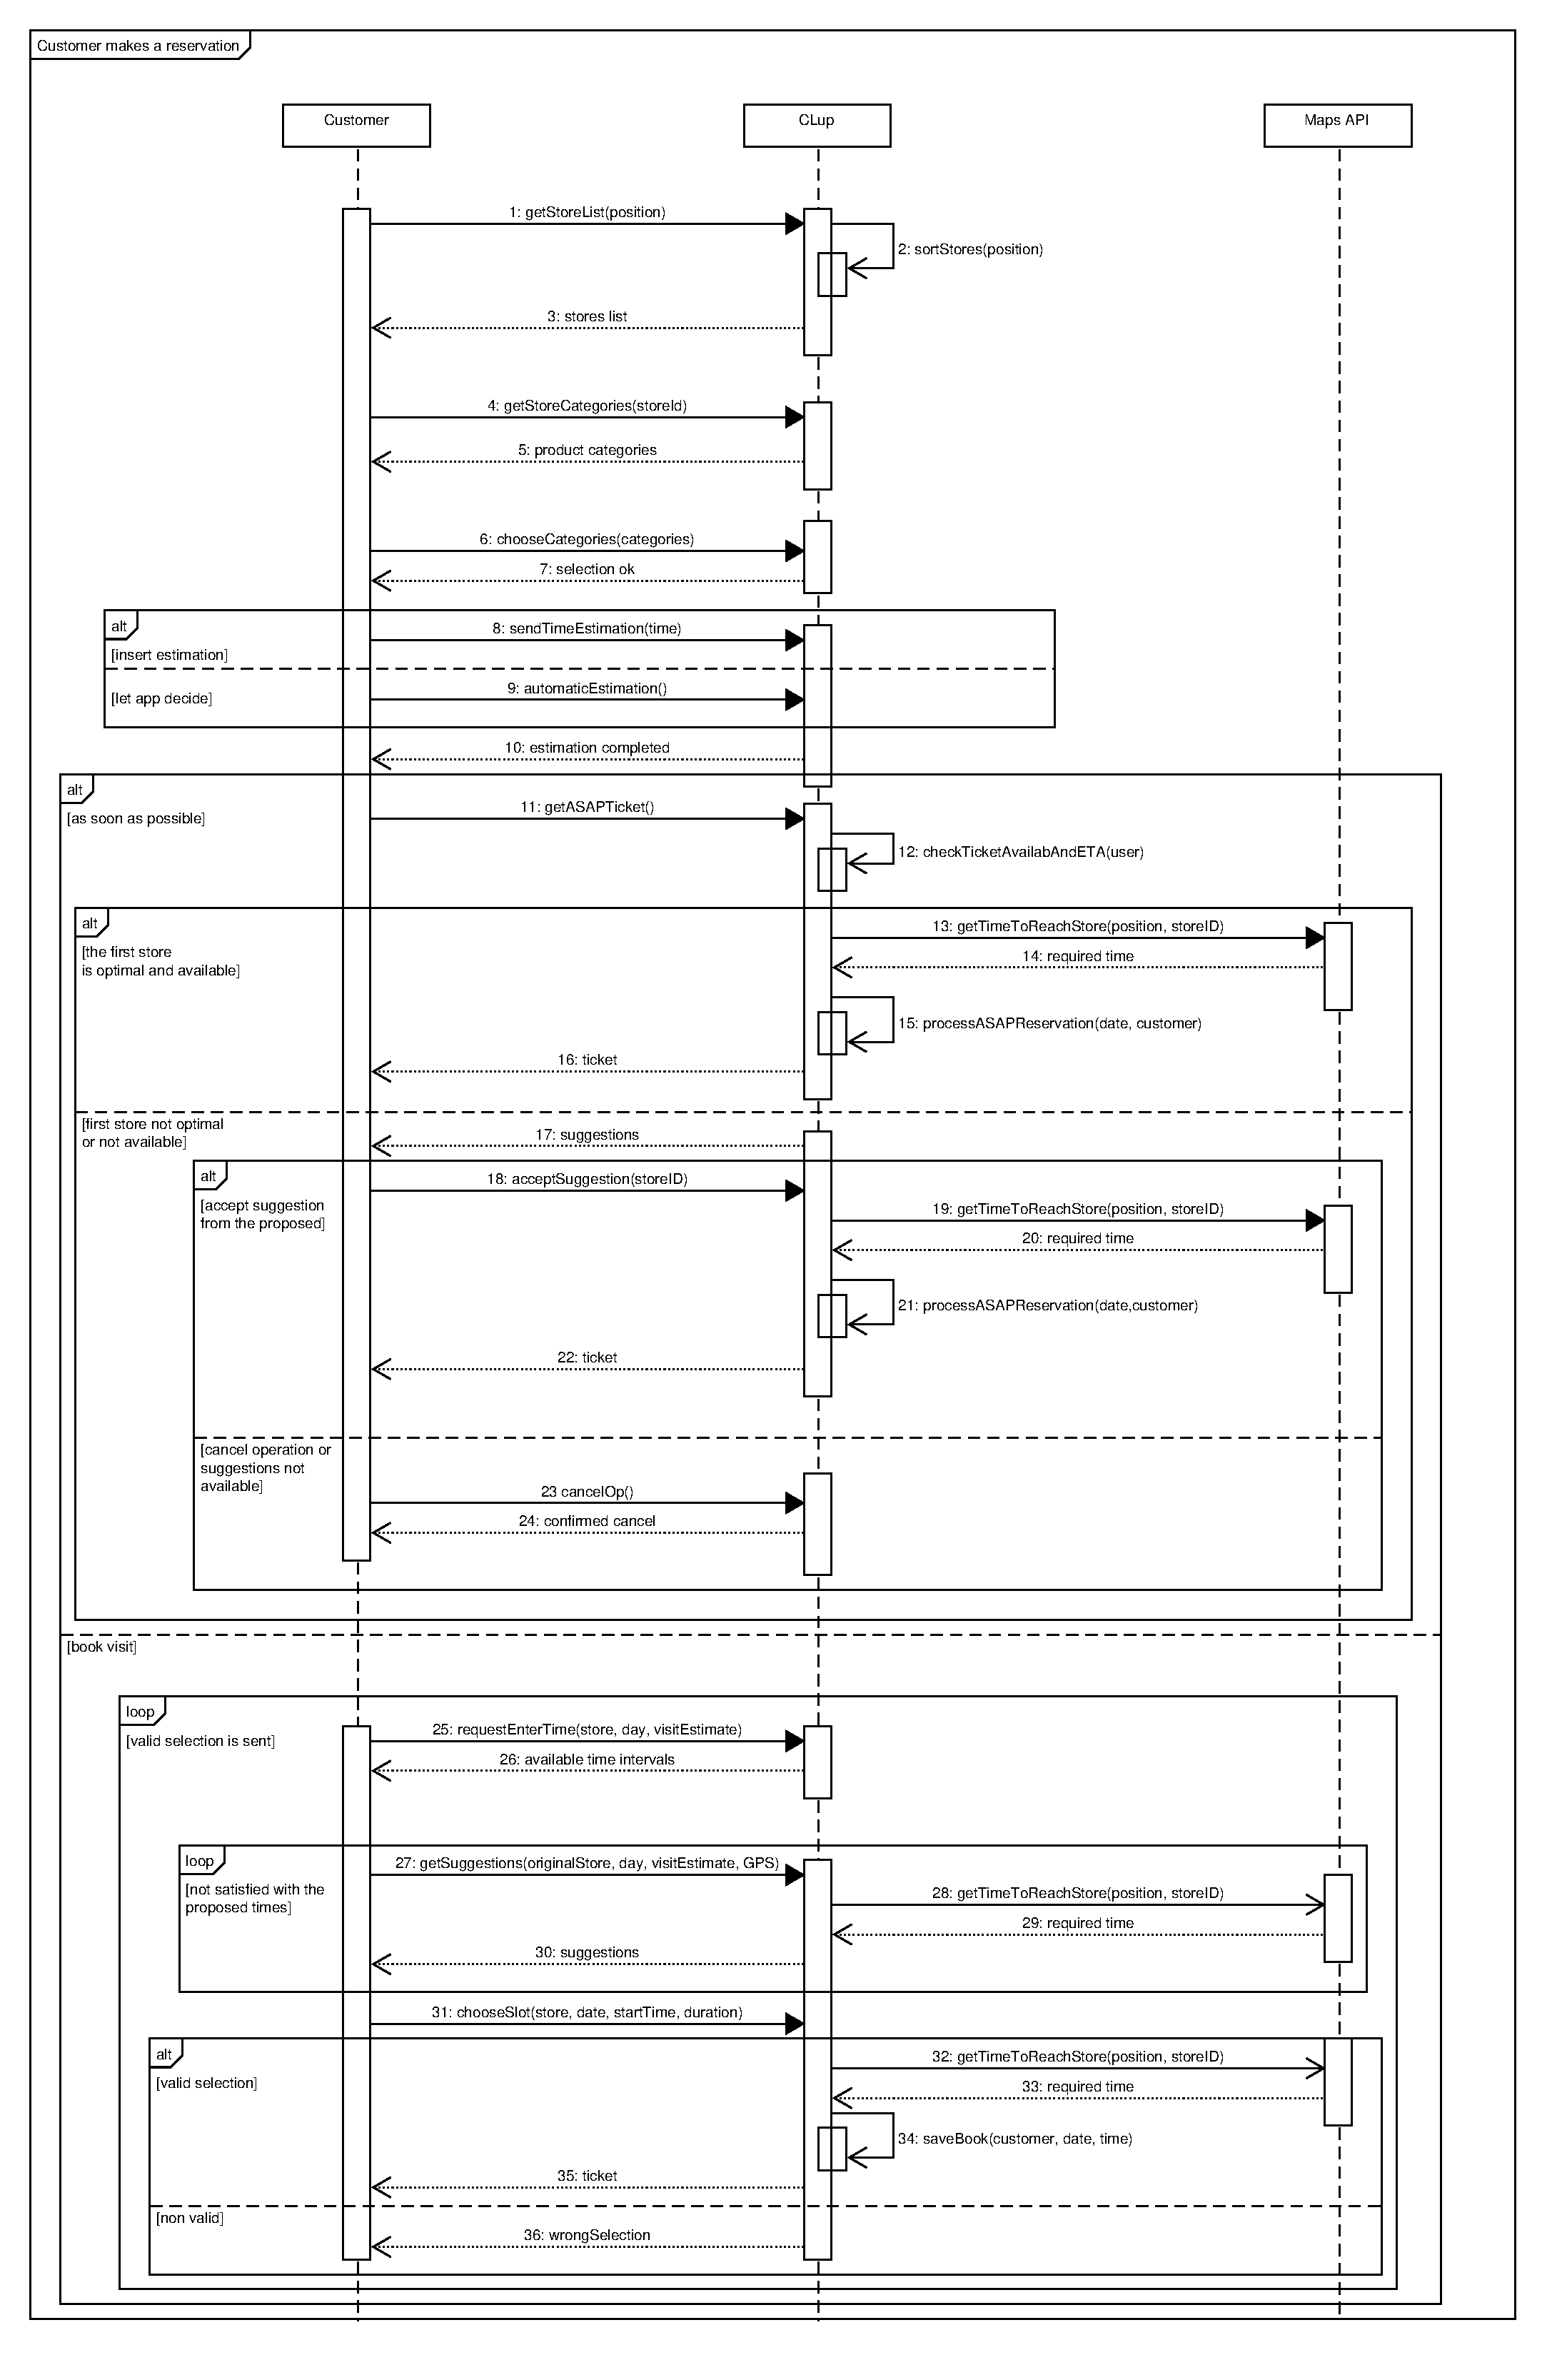
\includegraphics[scale=0.33]{SD/5_makeReservation.pdf}\\
									\caption{\emph{Sequence Diagram of Getting Ticket from App Procedure}}
								\end{adjustwidth}
							\end{figure}

					\begin{itemize}
					\bigskip
					\bigskip
					\bigskip
					 {\bfseries Required functional requirements: }


					\item {\bfseries R9}: The system allows the customers to select some or all the departments in which the customers are interested in doing shopping
					\item {\bfseries R12}: The system must show the customers of the time periods in which they can
					enter the store, accordingly to the estimate of customers' shopping time
					\item {\bfseries R13}: The system have to make a reasonable estimate of when a user with a spot on the queue is able to enter the store
					\item {\bfseries R15}: The system is able to ask for the position of the customers
					\item {\bfseries R22}: The system knows the situation in real time of each store
					\item {\bfseries R23}: The system takes trace of each customer entry and exit from the store
					\item {\bfseries R24}: The system contains a list of bookable stores
					\item {\bfseries R26}: The system can reasonably estimate the time needed from a specific user to complete his shopping
					\item {\bfseries R27}: The system saves clients' tickets


					\end{itemize}
				\end{center}
			
			\paragraph{Customer visualizes reservations}
			
				\begin{center}
					
					\rowcolors{2}{}{gray!20}
					\rowcolors{1}{gray!20}{white}
					
					\begin{adjustwidth}{-3cm}{}
					\begin{tabular}[h!]{|m{7.5em}|m{36em}|}
						
						\hline
						\xrowht{5pt}
						Name & Customer visualizes reservations\\
						\xrowht{5pt}
						Actors & Customer\\
						\xrowht{5pt}
						Entry Condition & Customer is already logged in the application service\\
						\xrowht{5pt}
						Event Flow & \begin{enumerate}
							
							\itemsep-0.25em
							\item Customer clicks on “Show requests” button
							\item The app show the list of bookings made and tickets requested
							\item The customer select the desired option
							\item The system opens the detail page of the selected option, that includes the “\emph{QR Code}” and the number that should be called, among with the real time entry date and time and time needed to reach the store. 
							
						\end{enumerate}\\
						\xrowht{5pt}
						Exit Conditions & Customer can visualize the reservation\\
						\xrowht{5pt}
						Exception & \begin{enumerate}
						\item The client has not pending requests
						\newline
						If the above situation happen, the app shows an error message and bring the client to the home page.
						\item The internet connection is not available
						\newline
						If the above situation happen, the app will load the local cached informations.
						\end{enumerate}	
\\
						\hline
						
					\end{tabular}
					\end{adjustwidth}

					\newpage
					
					\begin{itemize}
					\bigskip
					\bigskip
					\bigskip
					 {\bfseries Required functional requirements: }


					\item {\bfseries R5}: The system allows the customers to view their visits
					\item {\bfseries R8}: The system allows the customers to select their favourite means of transportation
					\item {\bfseries R13}: The system have to make a reasonable estimate of when a user with a spot on the queue is able to enter the store
					\item {\bfseries R15}: The system is able to ask for the position of the customers
					\item {\bfseries R27}: The system saves clients' tickets

					
					\end{itemize}
				\end{center}
					\begin{figure}
						\begin{adjustwidth} {-1cm}{}
							\centering
							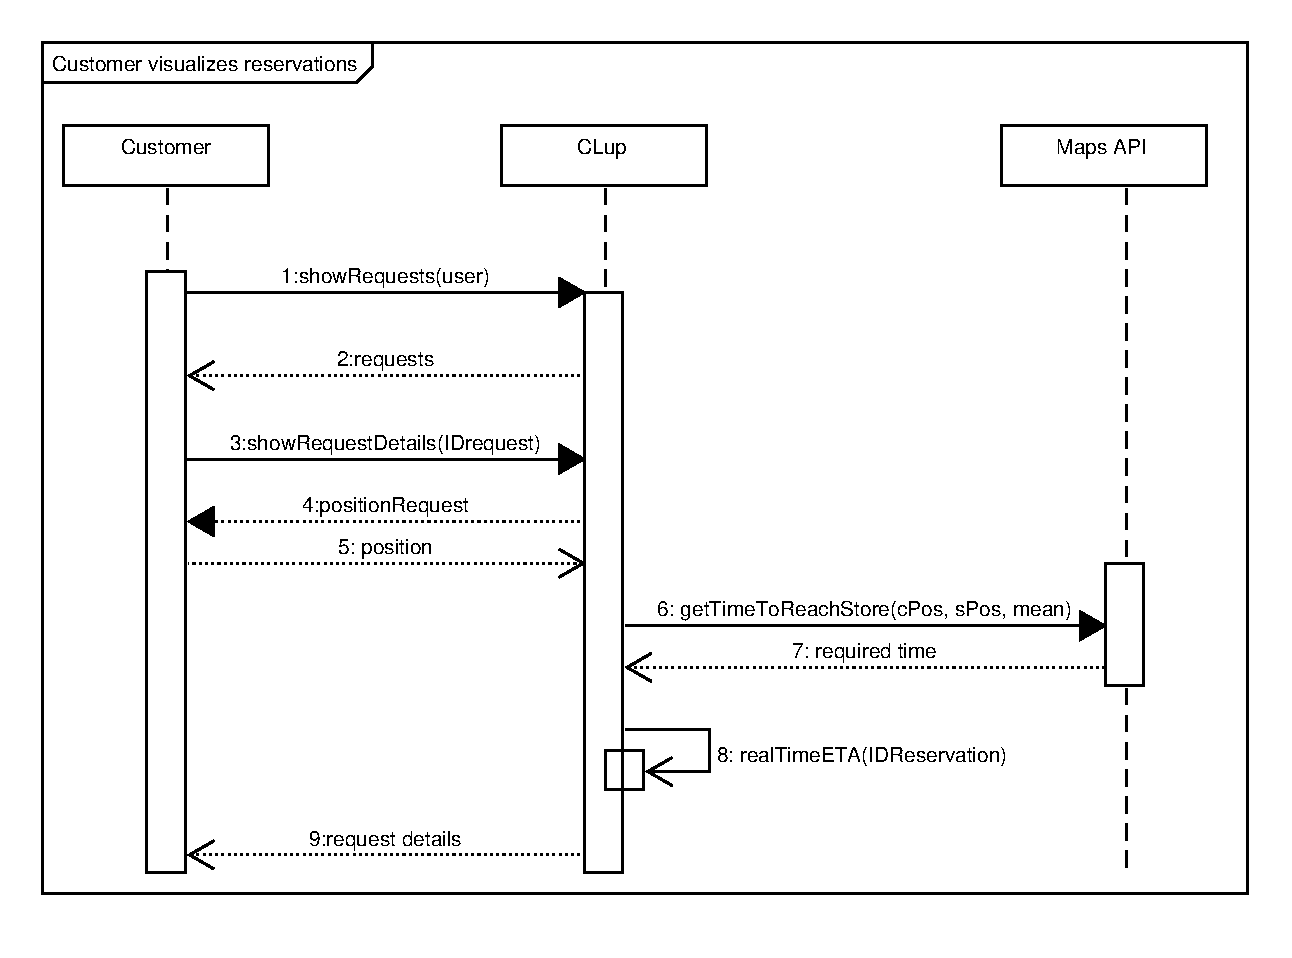
\includegraphics[scale=0.65]{SD/6_visualizeReservation.pdf}\\
							\caption{\emph{Sequence Diagram of Visualizing Customers' Reservations in app}}
						\end{adjustwidth}
					\end{figure}
			\newpage
			\paragraph{Manager modifies store parameters}
			
				\begin{center}
					
					\rowcolors{2}{}{gray!20}
					\rowcolors{1}{gray!20}{white}
					
					\begin{adjustwidth}{-3cm}{}
					\begin{tabular}[h!]{|m{7.5em}|m{36em}|}
						
						\hline
						\xrowht{5pt}
						Name & Store manager modifies store parameters\\
						\xrowht{5pt}
						Actors & Store manager\\
						\xrowht{5pt}
						Entry Condition & Store manager is already logged in the application service\\
						\xrowht{5pt}
						Event Flow & \begin{enumerate}
							
							\itemsep-0.25em
							\item Store manager clicks on “Modify parameters” button
							\item Store manager can see both the parameters relatives to the whole store (eg. ID, Pwd, Working Hours for the selected day of the week), and each department with its parameters (max capacity and simultaneous allowed bookings)
							
							\begin{enumerate}
								
								\itemsep0em
								\item Store manager can choose a day of the week using the "Change Day" button, if the currently selected is of no interest to him and have to modify some options on store's working hours.
								\item Store manager modify one, more or none of the parameters of the store or of some departements (clicking on the pencil shaped button of the desidered department) (remind that only working hours are dependent on the selected day)
								\item Store manager choose to add/delete some department respectively clicking on "Add a department" and on the bin shaped button of the desidered department
								\item Store manager clicks on Save Changes
					
								
							\end{enumerate}
							\item The system saves and processe the changes (notifying clients if necessary) and bring him back to “Store menu” page
							
						\end{enumerate}\\
						\xrowht{5pt}
						Exit Conditions & Store manager has successfully updated store parameters\\
						\xrowht{5pt}
						Exception & \begin{enumerate}
							
							\itemsep-0.25em
							\item Store managers enters an invalid value for one or more parameters
							\item The store manager tries to add an already existing department

							
						\end{enumerate}
					
						If the above situation occur, the application will throw an error message and will return to “Modify parameters” page\\	
						\hline
						
					\end{tabular}
					\end{adjustwidth}

					\begin{itemize}
					\bigskip
					\bigskip
					{\bfseries Required functional requirements: }

					\item {\bfseries R14}: The system can send notification to the clients
					\item {\bfseries R16}: The system permits to store manager to modify some critical parameters of the store
					related to customers' affluence management
					\item {\bfseries R17}: The system allows the manager to establish the maximum simultaneously allowed booked clients in a specific department

					\item {\bfseries R21}: The store manager can handle the working days and hours of the store, for each day of the week
					\end{itemize}					

							\begin{figure}[!h]
								\begin{adjustwidth} {-1cm}{}
									\centering
									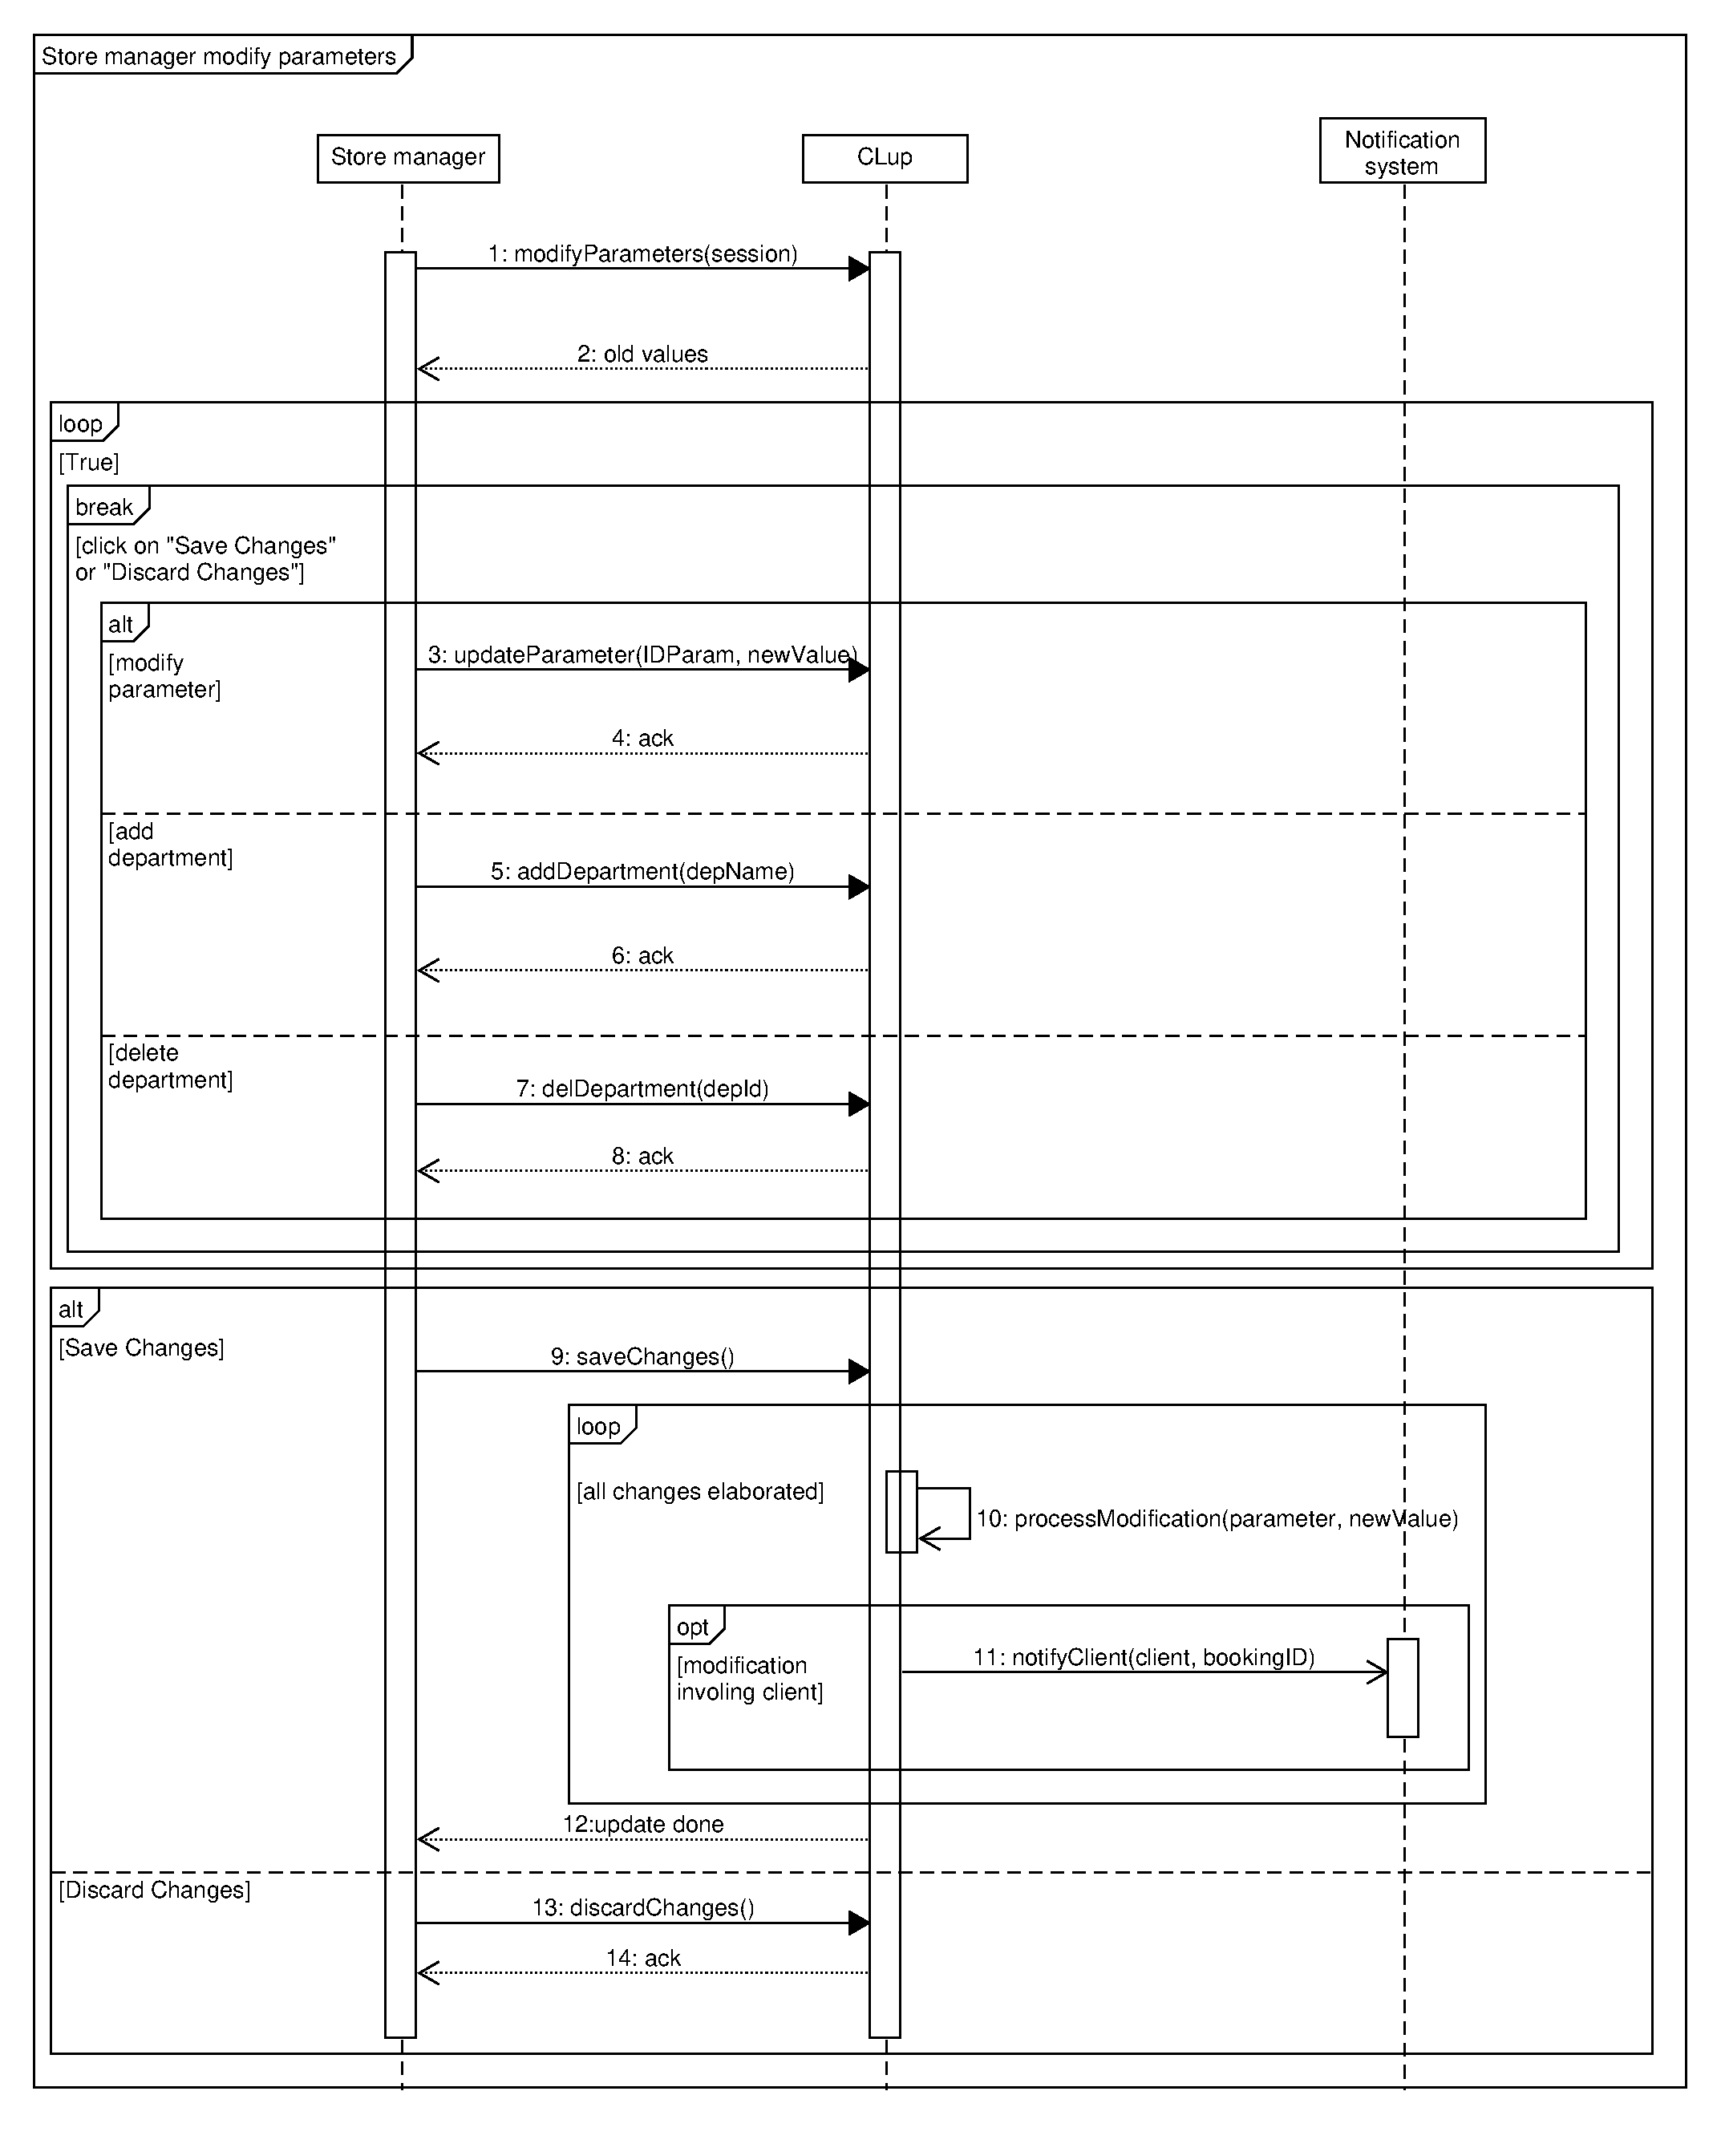
\includegraphics[scale=0.385]{SD/7_modifyParameters.pdf}\\
									\caption{\emph{Sequence Diagram of Visualizing Customers' Reservations in app}}
								\end{adjustwidth}
							\end{figure}
				\end{center}



			\newpage
			
			\paragraph{The store manager monitors the store situation}
			
				\begin{center}
					
					\rowcolors{2}{}{gray!20}
					\rowcolors{1}{gray!20}{white}
					
					\begin{adjustwidth}{-3cm}{}
					\begin{tabular}[h!]{|m{7.5em}|m{36em}|}
						\hline
						\xrowht{5pt}
						Name & Store manager monitors store situation\\
						\xrowht{5pt}
						Actors & Store manager\\
						\xrowht{5pt}
						Entry Condition & Store manager has opened the app and is already logged in\\
						\xrowht{5pt}
						Event Flow & \begin{enumerate}
							
							\itemsep-0.25em
							\item Manager clicks on “Monitor store” button
							\item The app shows a page with statistics on the store, including number of people inside the store, percentage of store occupation and the number of daily access to the building
							
							\begin{enumerate}
								\item If the manager wants, he can see the same statistics per store zone by clicking the “monitor zones” button. The system will show all the zones sorted by criticity
							\end{enumerate}
							
						\end{enumerate}\\
						\xrowht{5pt}
						Exit Conditions & Store manager can see statistics on the store\\
						\xrowht{5pt}
						Exception & None\\	
						\hline
						
					\end{tabular}
					\end{adjustwidth}
				
				\begin{itemize}
					\bigskip
					\bigskip
					{\bfseries Required functional requirements: }
					
					
					\item {\bfseries R9}:  The system allows the customers to select some or all the departments in which the customers are interested in doing shopping
					\item {\bfseries R23}: The system takes trace of each customer entry and exit from the store
				
				\end{itemize}
			
					\begin{figure}[!h]
						\begin{adjustwidth} {0cm}{}
							\centering
							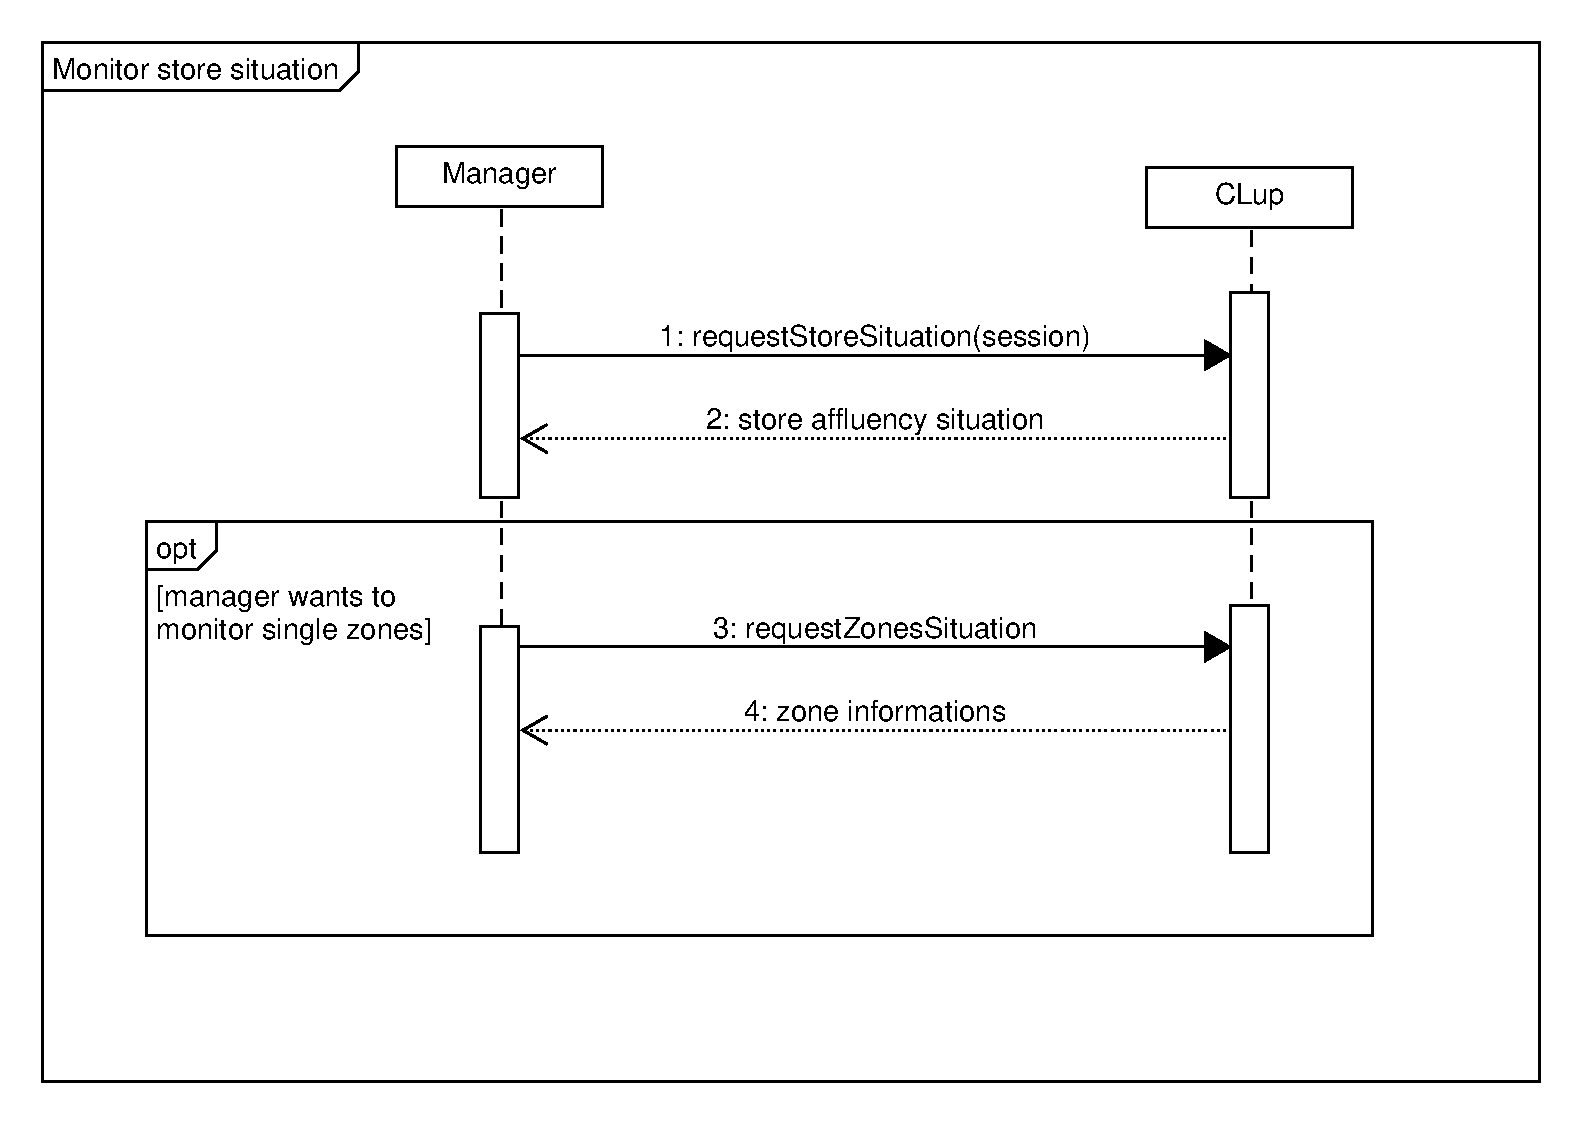
\includegraphics[scale=0.25]{SD/8_monitorStoreSituation.pdf}\\
							\caption{\emph{Sequence Diagram of Visualizing Store and Departments Situation}}
						\end{adjustwidth}
					\end{figure}
					
				\end{center}
			
			\newpage
			\paragraph{The store manager manages customers bookings}
			
				\begin{center}
					
					\rowcolors{2}{}{gray!20}
					\rowcolors{1}{gray!20}{white}
					
					\begin{adjustwidth}{-3cm}{}
						\begin{tabular}[h!]{|m{7.5em}|m{36em}|}
							\hline
							\xrowht{5pt}
							Name & The store manager manages customers bookings\\
							\xrowht{5pt}
							Actors & Store manager\\
							\xrowht{5pt}
							Entry Condition & Store manager has opened the app and is already logged in\\
							\xrowht{5pt}
							Event Flow & \begin{enumerate}
								
								\itemsep-0.25em
								\item Manager clicks on “Manage bookings” button
								\item The app shows a list of reservations, with some of their details in preview (such as chosen date and time slot)
								\item The manager can choose one of them, and the app will show some possibilities to the manager
								
								\begin{enumerate}
									
									\item The manager can press on the button “Contact client” to contact the client for some reasons.
									
									\begin{enumerate}	
											
											\item The app will show an interface where the manager can insert the email text
											\item The manger clicks on the “Send” button to send the email

										\item The app returns to the previous page
										
										
									\end{enumerate}
								
									\item The manager can click on the button “Cancel booking” to cancel a reservation
									
									\begin{enumerate}
										
										\item The app will show a dialog box where the manager can put-in an optional message, explaining the reasons of the cancel
										\item The manager clicks on the “Delete button”
										\item The app will show a confirmation box to ask if the manager is sure to proceed
										\item The manager clicks on “Yes” to confirm the deletion, and notifies the customer
										\item The app closes the dialog box
										
									\end{enumerate}
								
									\item The manager can choose to reschedule a booking
									
									\begin{enumerate}
										
										\item The app will show a dialog box where the manager can choose a new time slot and insert a message explaining the reasons
										\item The manager clicks on “Modify” to modify the booking
										\item The app closes the dialog box
										
									\end{enumerate}
									
								\end{enumerate}
								
							\end{enumerate}\\
							\xrowht{5pt}
							Exit Conditions & Store manager can manage the store and is able to edit reservations\\
							\xrowht{5pt}
							Exception & \begin{enumerate}
								
								\itemsep-0.25em
								\item There isn't any reservation
							\end{enumerate}
							If the above situation occur, the app will show a dialogue box with an error message. \\	
							\hline
							
						\end{tabular}
					\end{adjustwidth}
				\newpage
					\begin{figure}[!h]
						\begin{adjustwidth} {-1.3cm}{}
							\centering
							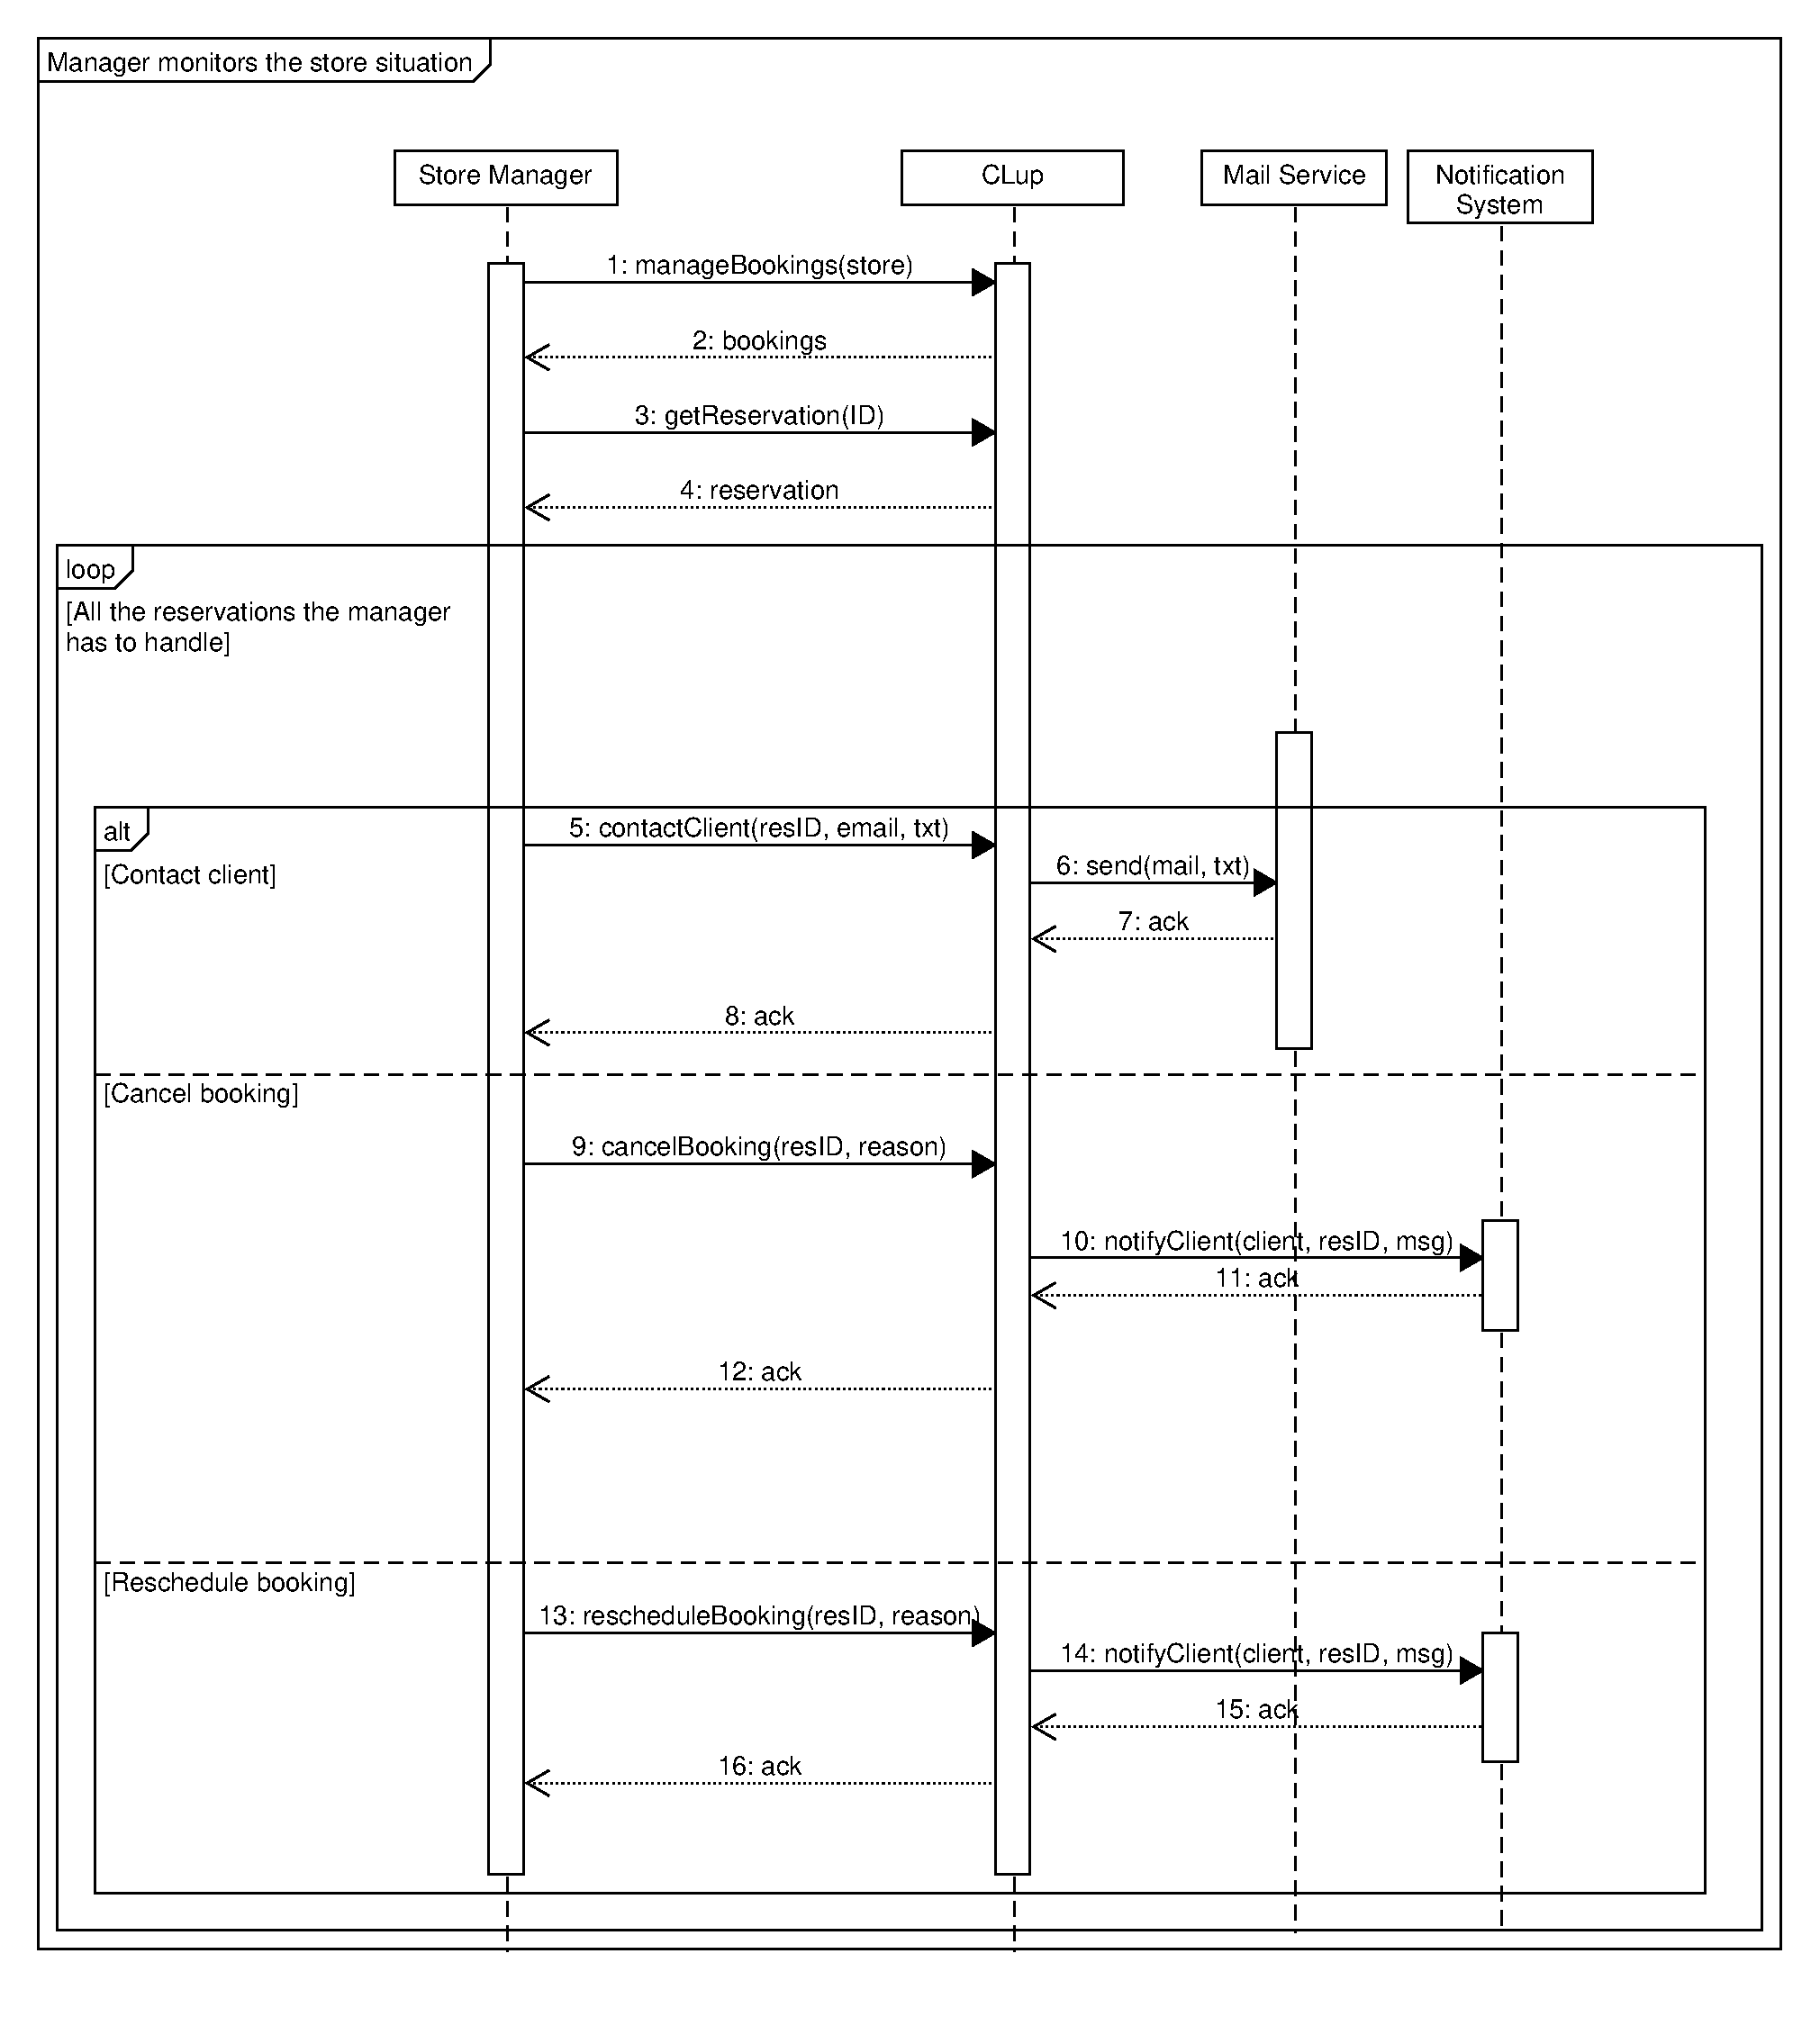
\includegraphics[scale=0.42]{SD/9_manageReservations(store)}\\
							\caption{\emph{Sequence Diagram of Visualizing Store and Departments Situation}}
						\end{adjustwidth}
					\end{figure}
					\begin{itemize}
						\medskip
						
						{\bfseries Required functional requirements: }
						
						\item {\bfseries R14}: The system can send notification to the clients
						\item {\bfseries R18}: The store manager can view the reservation of each client
						\item {\bfseries R19}: The store manager can modify the reservation of each client
						\item {\bfseries R20}: The store manager can cancel the reservation of each client
						\item {\bfseries R27}: The system saves clients' tickets
						\item {\bfseries R30}: The system is able to send emails
						\item{\bfseries R32}: The system can automatically rearrange reservations, if necessary
						

					\end{itemize}	
					
				\end{center}
			
			\paragraph{Customers reservations management}
			
				\begin{center}
					
					\rowcolors{2}{}{gray!20}
					\rowcolors{1}{gray!20}{white}
					
					
					\begin{adjustwidth}{-3cm}{}
					\begin{tabular}[h!]{|m{7.5em}|m{36em}|}
							\hline
							\xrowht{5pt}
							Name & Customers reservations management\\
							\xrowht{5pt}
							Actors & Customer\\
							\xrowht{5pt}
							Entry Condition & The customer has the application opened, is logged in and has at least one pending request\\
							\xrowht{5pt}
							Event Flow & \begin{enumerate}
								
								\itemsep-0.25em
								\item The user press on the “Show requests” button
								\item The app shows a page with the requests made by the client
								\item The user selects the desidered requests
								\item The app will show the requests details
								\item The user press the “edit” button
								
								\begin{enumerate}
									
									\item If the selected requests is a ticket, the customer can delete it pressing the “Delete button”
									
									\begin{enumerate}
										
										\item The system will show a confirmation dialogue
										\item The client press the yes button
										\item The ticket is deleted and the app will return to the previous screen if there are other requests, or to the main menu otherwise
										
									\end{enumerate}
								
									\item If the selected request is a booking, the client can both click the delete button, and follow the above procedure or can select the “modify button”
									
									\begin{enumerate}
										
										\item If the modify button is selected, the app ask the customer all the parameters asked when making a reservation. This parameters can be modified, and at the end the modification confirmed, or discarded.
										 
									\end{enumerate}
									
								\end{enumerate}
								
							\end{enumerate}\\
							\xrowht{5pt}
							Exit Conditions & The client can modify his reservation\\
							\xrowht{5pt}
							Exception & \begin{enumerate}
								
								\itemsep-0.25em
								\item There isn't any reservation
								\end{enumerate}
							If the above situation occur, the app will show a dialogue box with an error message.\\	
							\hline
							
						\end{tabular}
					\end{adjustwidth}
					\begin{itemize}
						\medskip
						\newpage
						{\bfseries Required functional requirements: }
						
						
						\item {\bfseries R5}: The system allows the customers to view their visits
						\item {\bfseries R6}: The system allows the customers to cancel their visits
						\item {\bfseries R7}: The system allows the customers to modify their visits		
						\item {\bfseries R8}: The system allows the customers to select their favourite means of transportation
						\item {\bfseries R9}: The system allows the customers to select some or all the departments in which the customers are interested in doing shopping
						\item {\bfseries R11}: The system must consider the estimate shopping time inserted by customers
						\item {\bfseries R12}: The system must show the customers of the time periods in which they can enter the
						store, accordingly to the estimate of customers' shopping time
						\item {\bfseries R13}: The system have to make a reasonable estimate of when a user with a spot	on the queue is able to enter the store
						\item {\bfseries R15}: The system is able to ask for the position of the customers
						\item {\bfseries R22}: The system knows the situation in real time of each store
						\item {\bfseries R26}: The system can reasonably estimate the time needed from a specific user to complete his shopping
						\item {\bfseries R27}: The system saves clients' tickets
						\item{\bfseries R32}: The system can automatically rearrange reservations, if necessary

					\end{itemize}
				

				\end{center}
			\newpage
			\begin{figure}[!htb]
				\begin{adjustwidth} {-3.8cm}{}
					\centering
					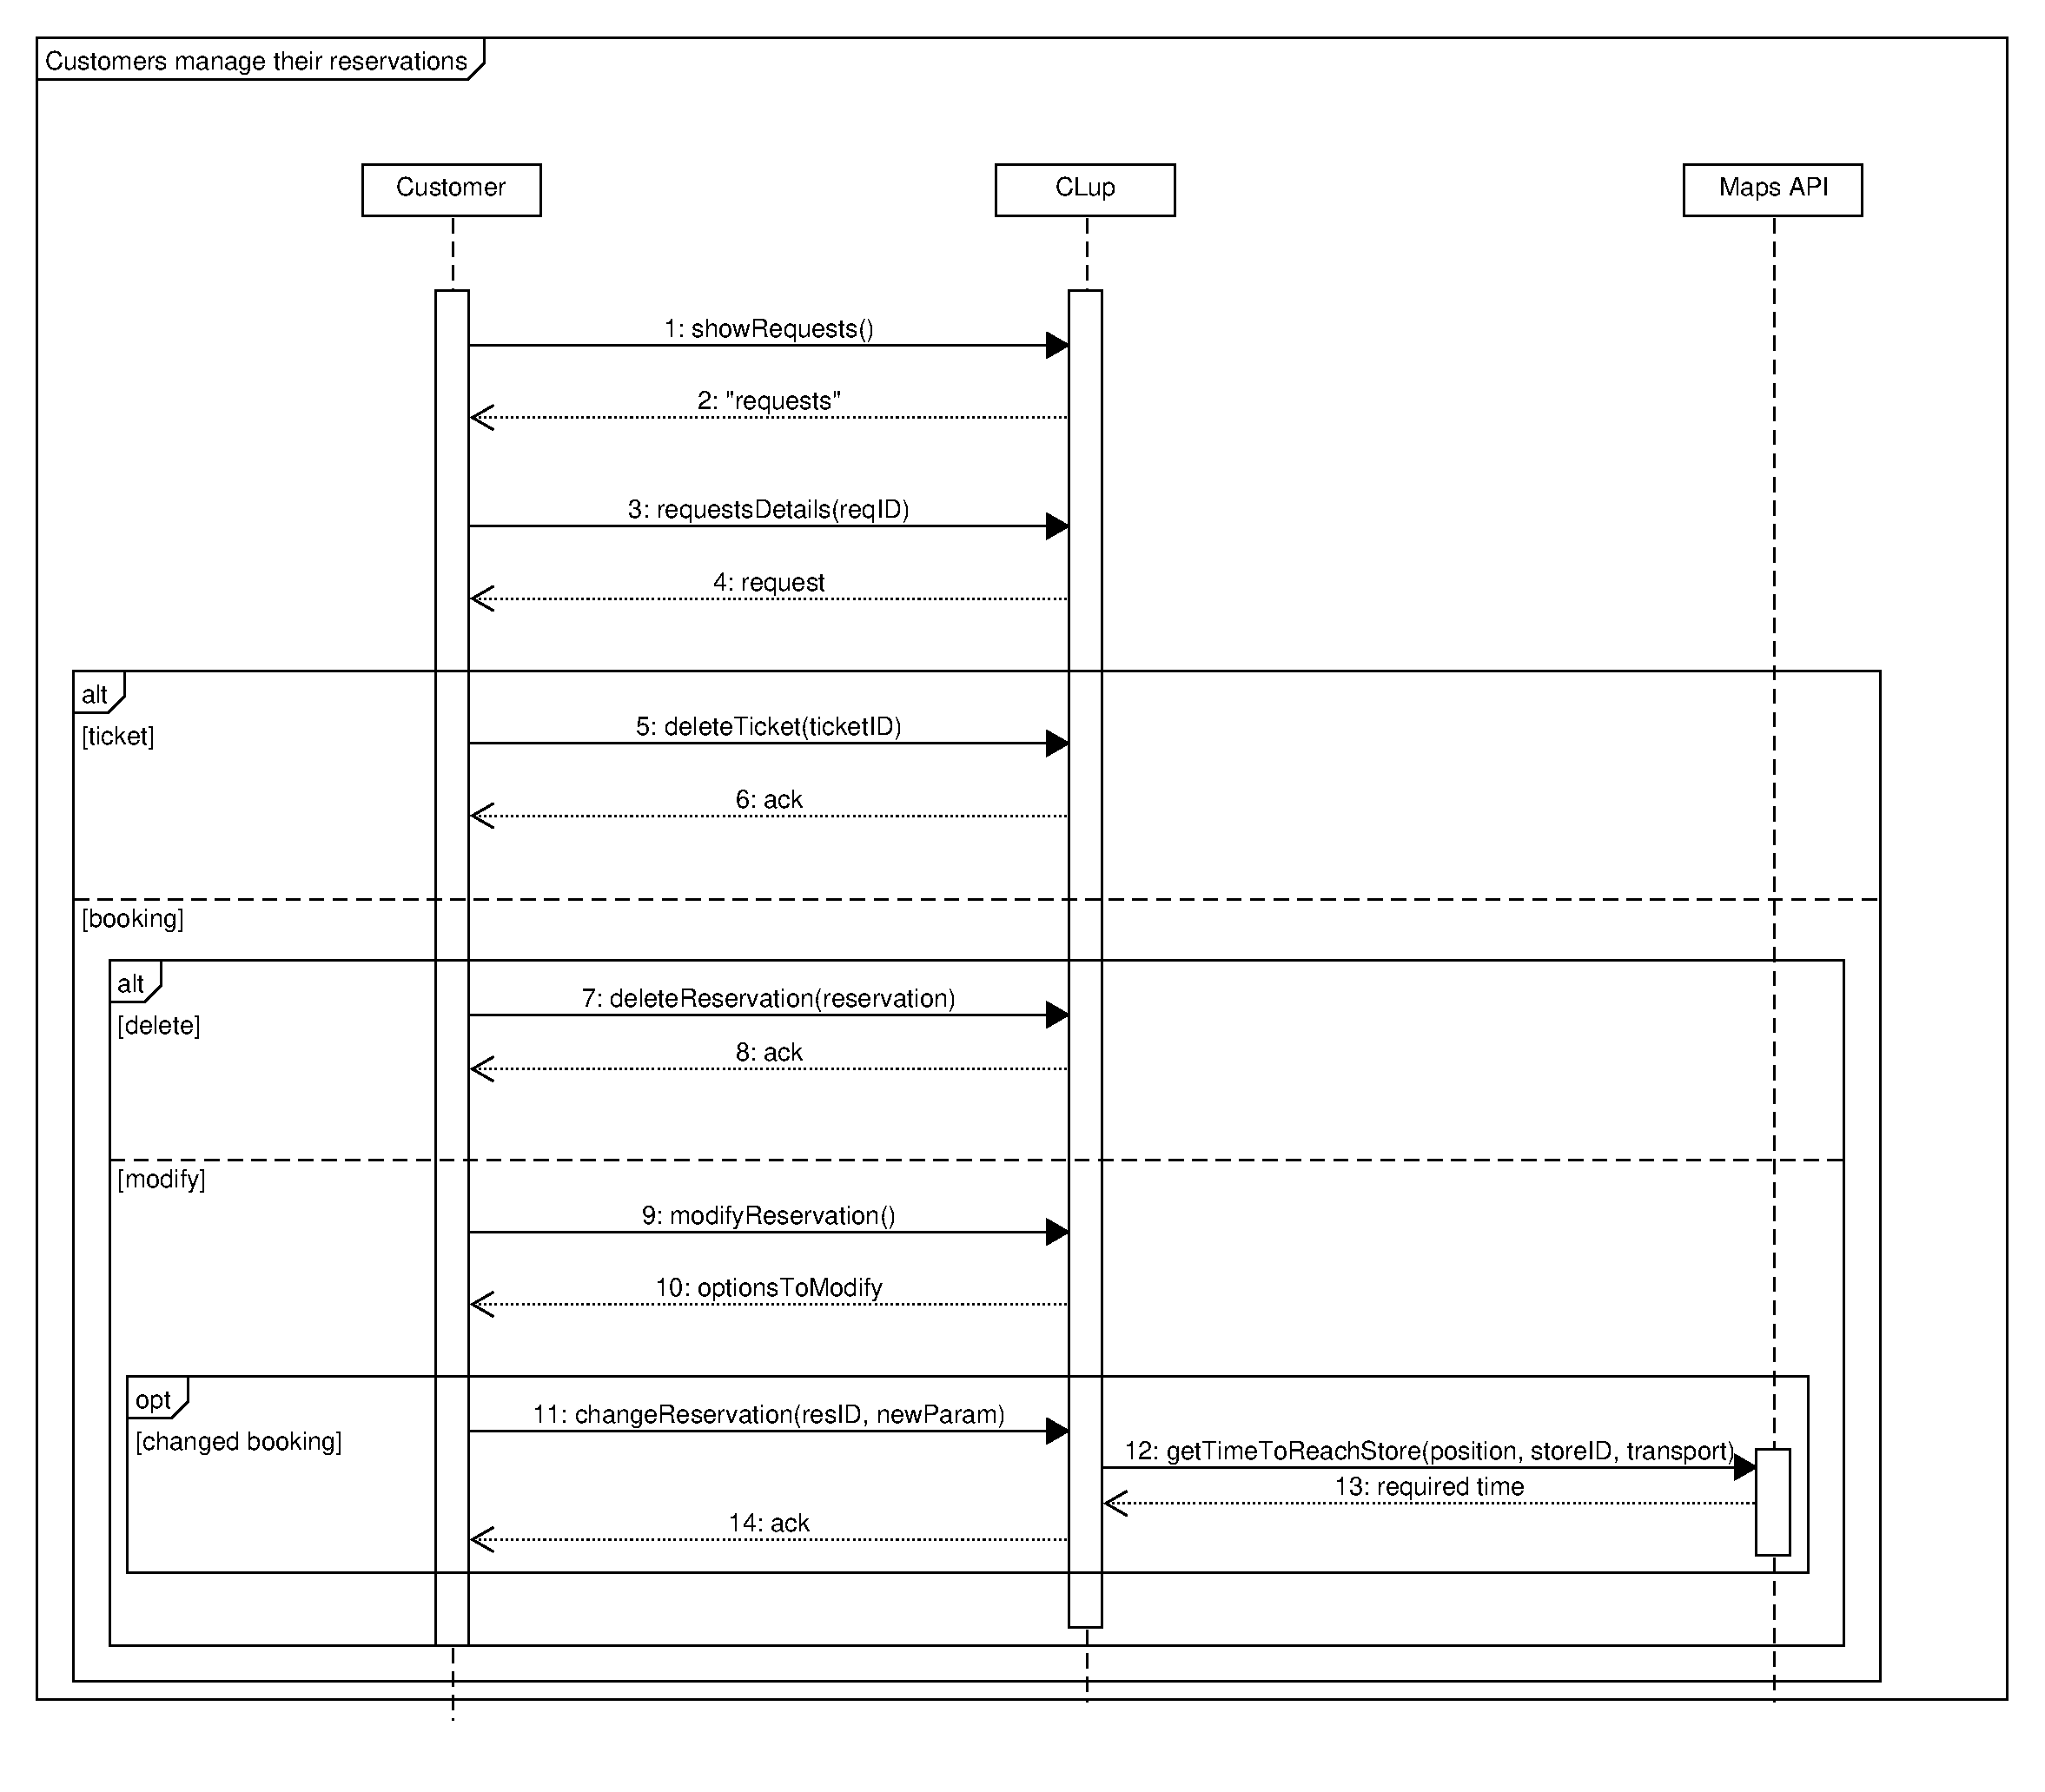
\includegraphics[scale=0.5]{SD/10_manageReservation(customer).pdf}\\
					\caption{\emph{Sequence Diagram of managing reservations customer side}}
				\end{adjustwidth}
			\end{figure}
		\newpage
		
			\paragraph{Customer get a ticket with the totem}
			
				\begin{center}
					
					\rowcolors{2}{}{gray!20}
					\rowcolors{1}{gray!20}{white}
					
					\begin{adjustwidth}{-3cm}{}
					\begin{tabular}[h!]{|m{7.5em}|m{36em}|}
							\hline
							\xrowht{5pt}
							Name & Customer get a ticket with the totem\\
							\xrowht{5pt}
							Actors & Customer\\
							\xrowht{5pt}
							Entry Condition & The customer is at the store and is using the totem \\
							\xrowht{5pt}
							Event Flow & \begin{enumerate}
								
								\itemsep-0.25em
								\item Customer clicks the button “Get Ticket”
								
								\item Customers can see the list of all possible objects’ categories and can select some of them (optional)
								
								\item The customer enters the estimation of shopping time, or let the system to infer it
								
								\item Client confirms the options selected and the system generates and prints the associated number, the \emph{QR Code} and the \emph{ETA}, with a warning if there is some risk on being able to enter only after the store is closed.
								
							\end{enumerate}\\
							\xrowht{5pt}
							Exit Conditions & The client gets a ticket \\
							\xrowht{5pt}
							Exception & \begin{enumerate}
								
								\item Client has not completed the operation in the prefixed time
								\item Client need more time to complete shopping than the remaining from the store's closing
								
							\end{enumerate}
						
							If the above situation occur, the application will throw an error message and will return to “Home” page \\
							\hline
							
						\end{tabular}

					\end{adjustwidth}
				
					\begin{itemize}
					\bigskip
					\bigskip
					\bigskip
					\bigskip
					{\bfseries Required functional requirements: }
					
					
					\item {\bfseries R9}: The system allows the customers to select some or all the departments in which the customers are interested in doing shopping
					\item {\bfseries R11}: The system must consider the estimate shopping time insert
					by customers
					\item {\bfseries R13}: The system have to make a reasonable estimate of when a user with a spot on the queue is able to enter the store
					\item {\bfseries R25}: The system is able to print a paper ticket
					\item {\bfseries R26}: The system can reasonably estimate the time needed from a specific user to complete his shopping
					\item {\bfseries R27}: The system saves clients' tickets

				\end{itemize}
					\begin{figure}[!htb]
						\begin{adjustwidth} {-3.2cm}{}
							\centering
							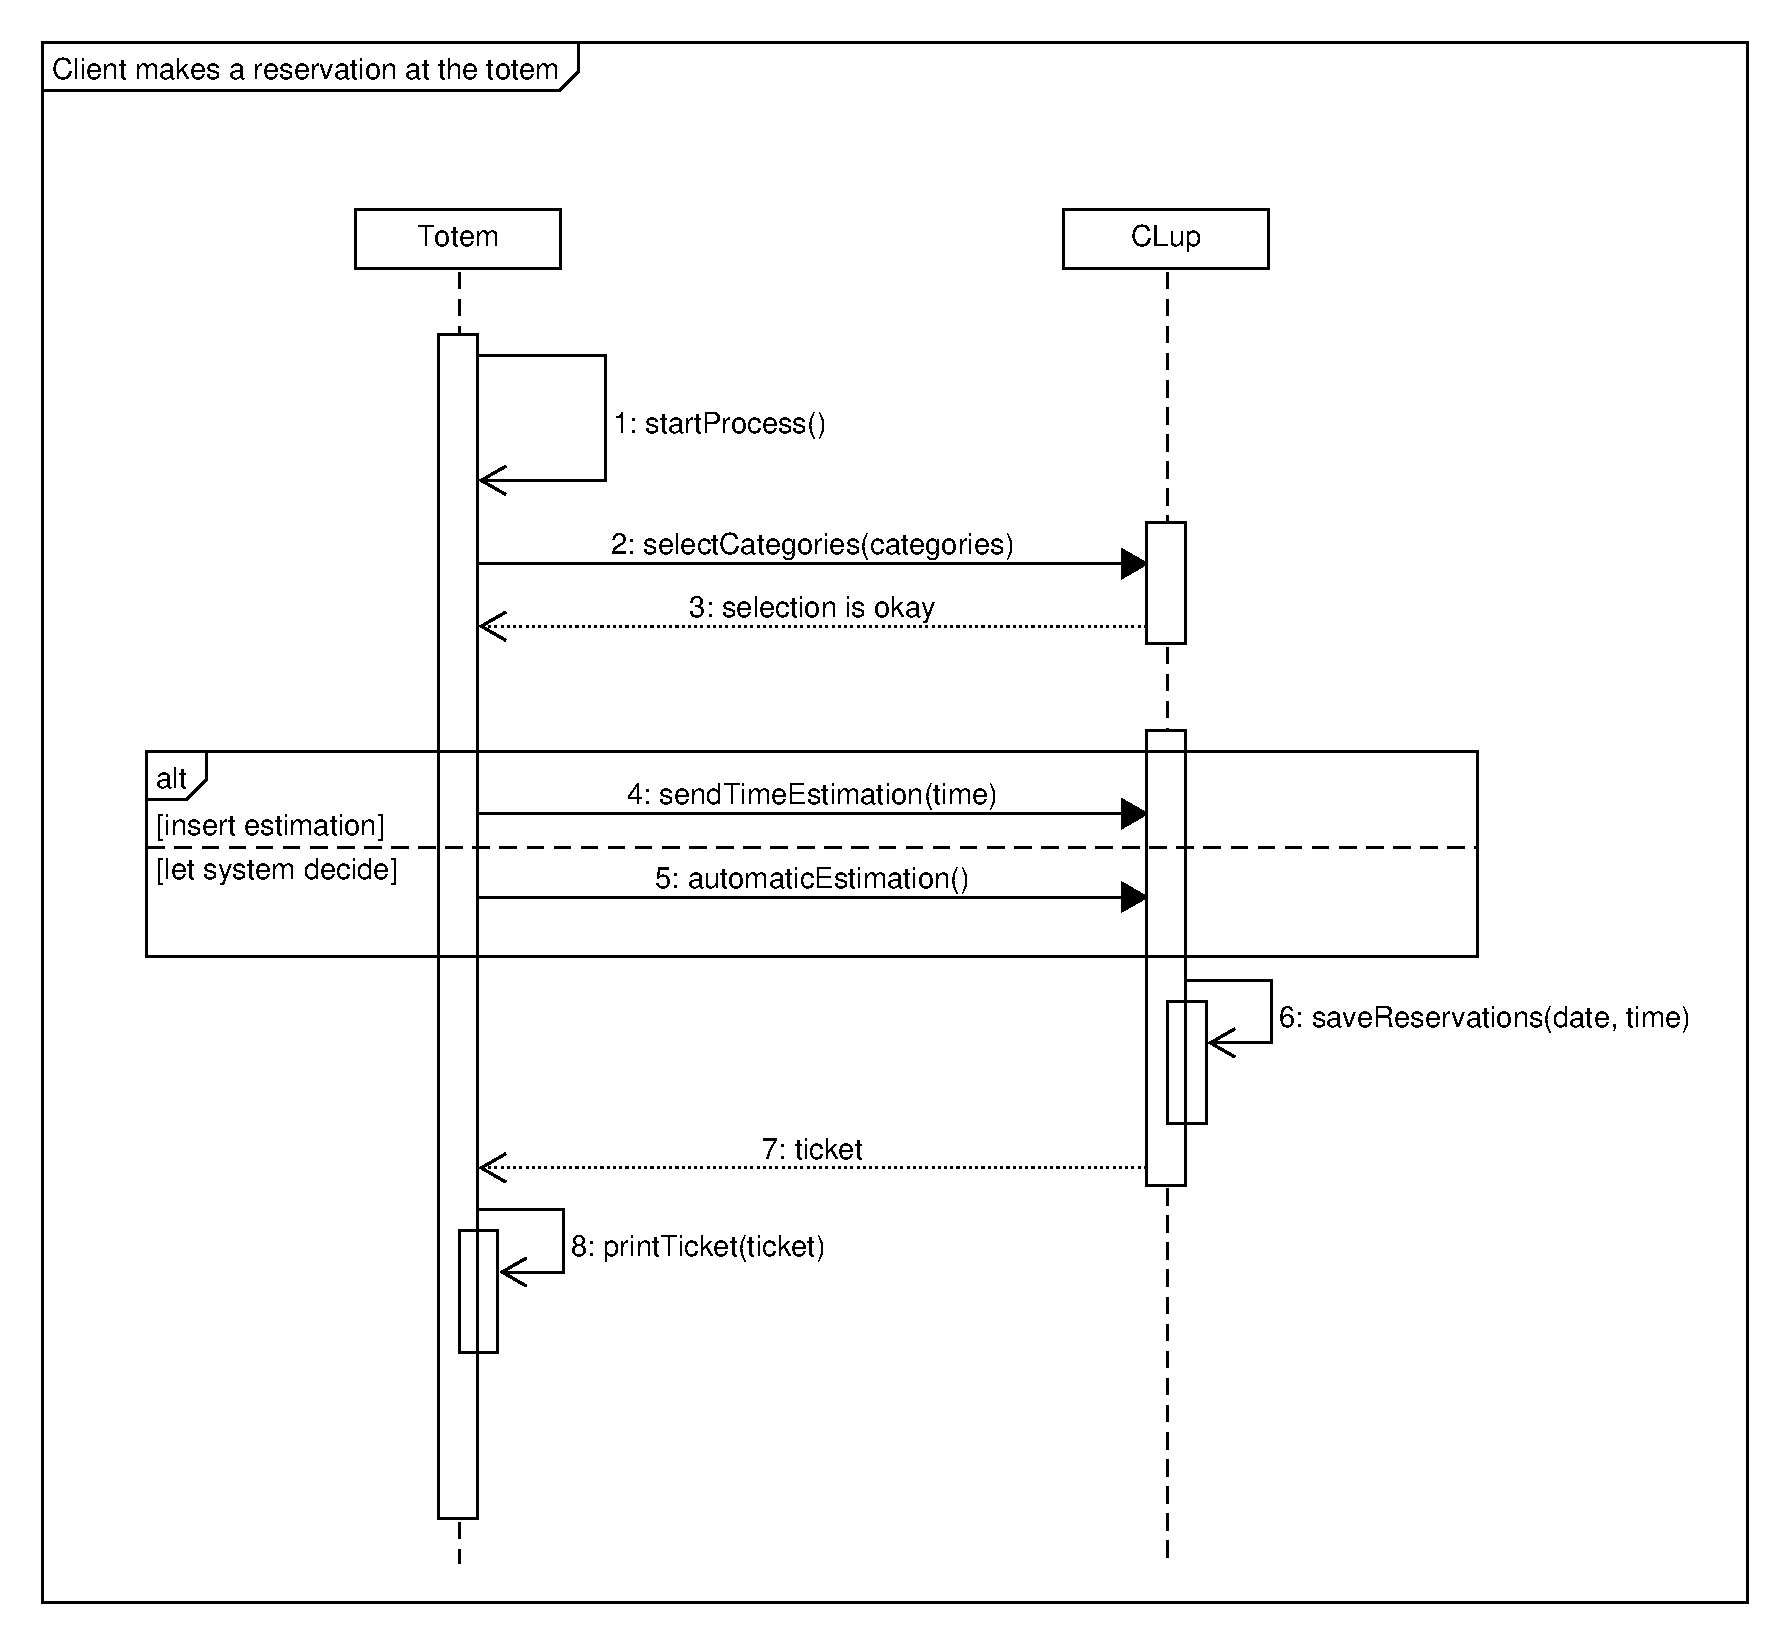
\includegraphics[scale=0.62]{SD/11_getTicketAtTotem.pdf}\\
							\caption{\emph{Sequence Diagram of getting a ticket at a physical dispenser}}
						\end{adjustwidth}
					\end{figure}
				\end{center}
			\newpage
			\paragraph{Customer selects the prefered means of transport}
			
				\begin{center}
					
					\rowcolors{2}{}{gray!20}
					\rowcolors{1}{gray!20}{white}
					
					\begin{adjustwidth}{-3cm}{}
						\begin{tabular}[h!]{|m{7.5em}|m{36em}|}
							\hline
							\xrowht{5pt}
							Name & Customer selects the preferred mean of transport \\
							\xrowht{5pt}
							Actors & Customer \\
							\xrowht{5pt}
							Entry Condition & Customer is already logged in the application service \\
							\xrowht{5pt}
							Event Flow & \begin{enumerate}
								
								\itemsep-0.25em
								\item Customer clicks the “Means of transport” button
								
								\item Customer can see a list of means of transport
								
								\item Customer select his preferred means of transport
								
								\item The system gets his \emph{GPS} positions and checks if the selected option is available.
								
								\item If the selected option is available, the app saves the option. Otherwise, shows an error message and invite the customer to repeat again the operation.
								
								 
								
							\end{enumerate}\\
							\xrowht{5pt}
							Exit Conditions & The client selects the preferred mean of transport \\
							\xrowht{5pt}
							Exception & None \\
							\hline
							
						\end{tabular}
					\end{adjustwidth}
					
					\begin{figure}[!htb]
						\begin{adjustwidth} {-0.5cm}{}
							\centering
							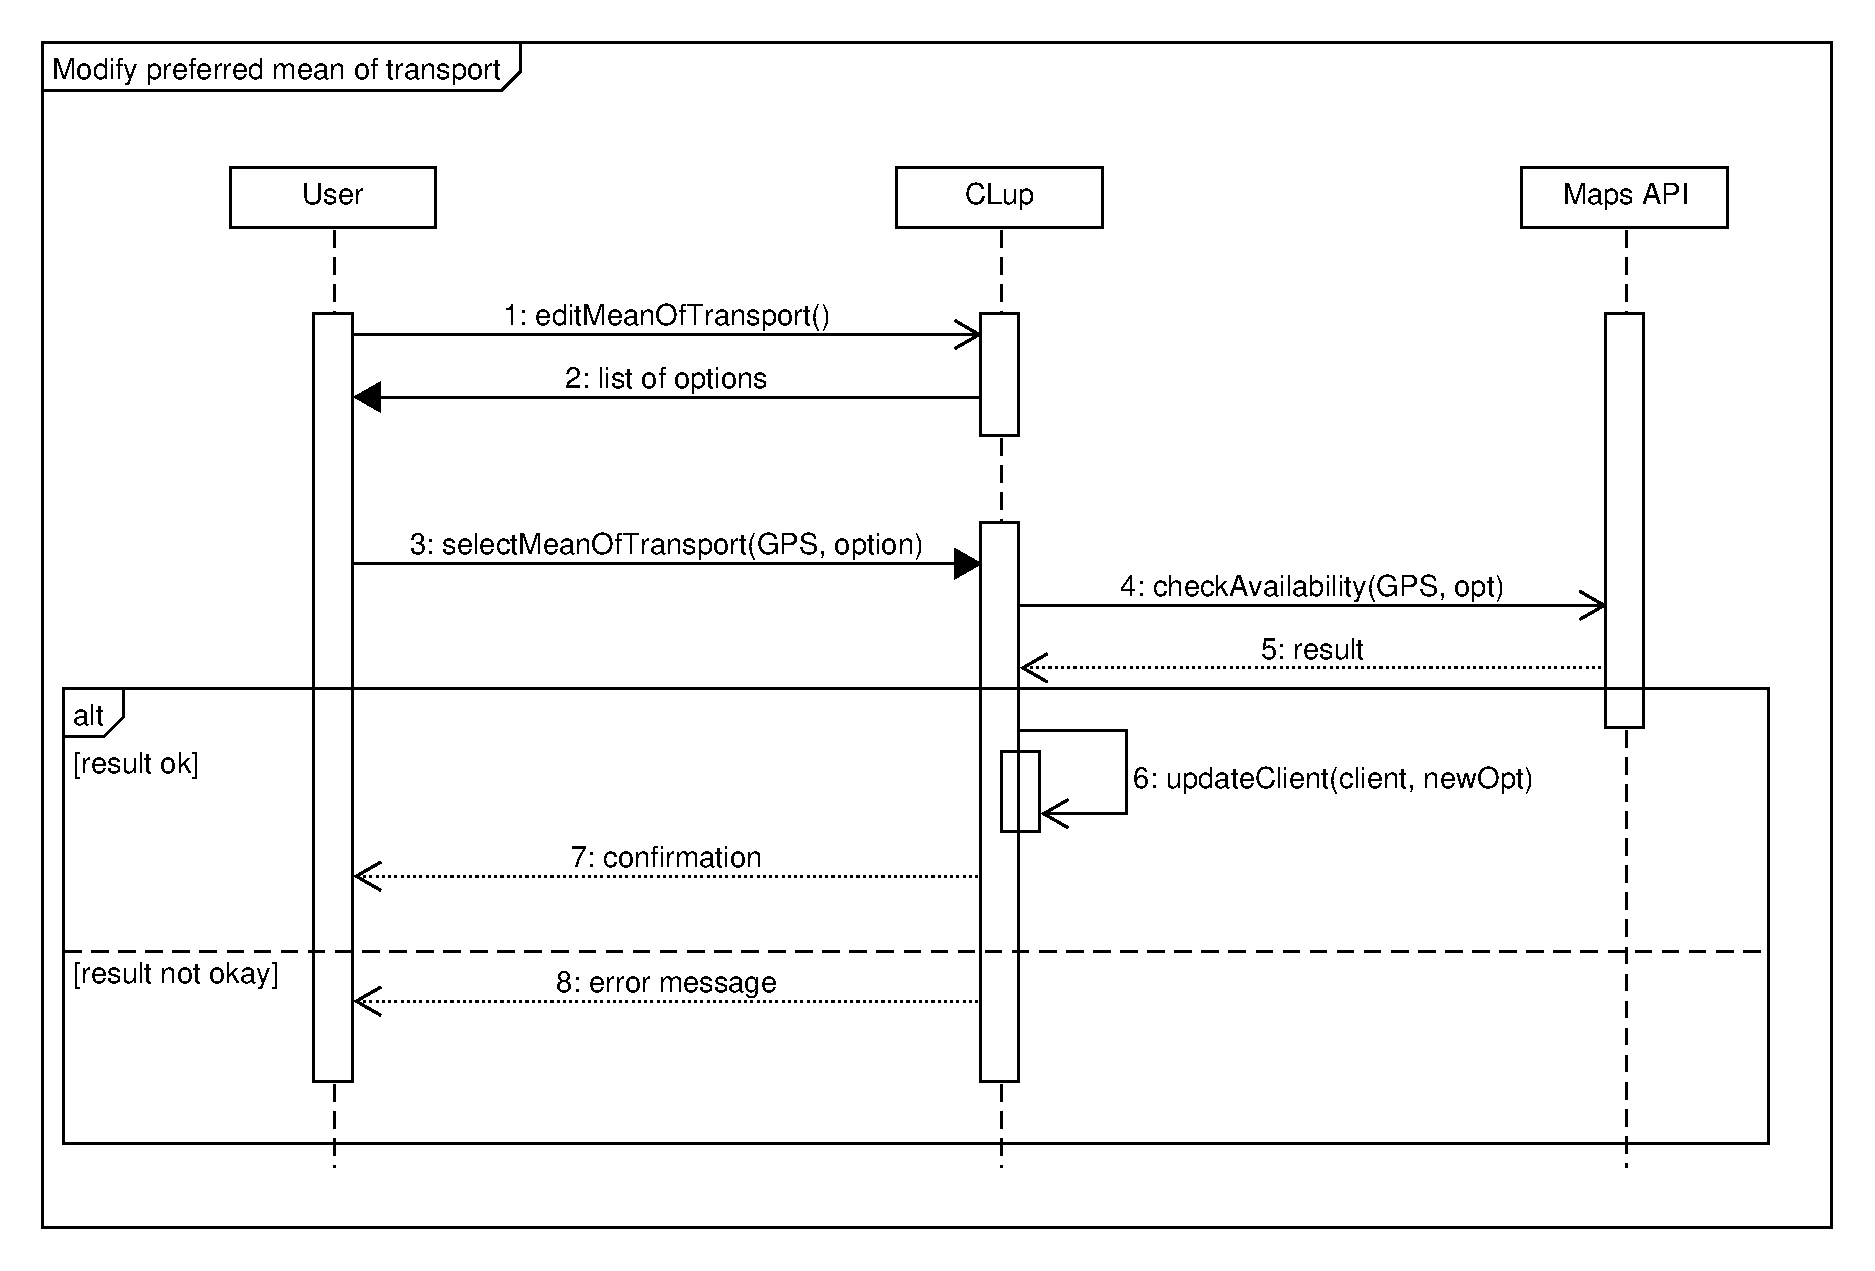
\includegraphics[scale=0.42]{SD/12_selectPreferredMeanOfTransport.pdf}\\
							\caption{\emph{Sequence Diagram of changing preferred mean of transport}}
						\end{adjustwidth}

					\end{figure}
					
					
					\begin{itemize}
						\medskip
						\newpage
						{\bfseries Required functional requirements: }
						
						
						\item {\bfseries R8}: The system allows the customers to select their favourite means of transportation
						\item {\bfseries R15}: The system is able to ask for the position of the customers
											
						
					\end{itemize}
				\end{center}
		
		\subsection{Use Case Diagram}
		
		\begin{figure}[!htb]
			\begin{adjustwidth} {-3,6cm}{}
				\centering
				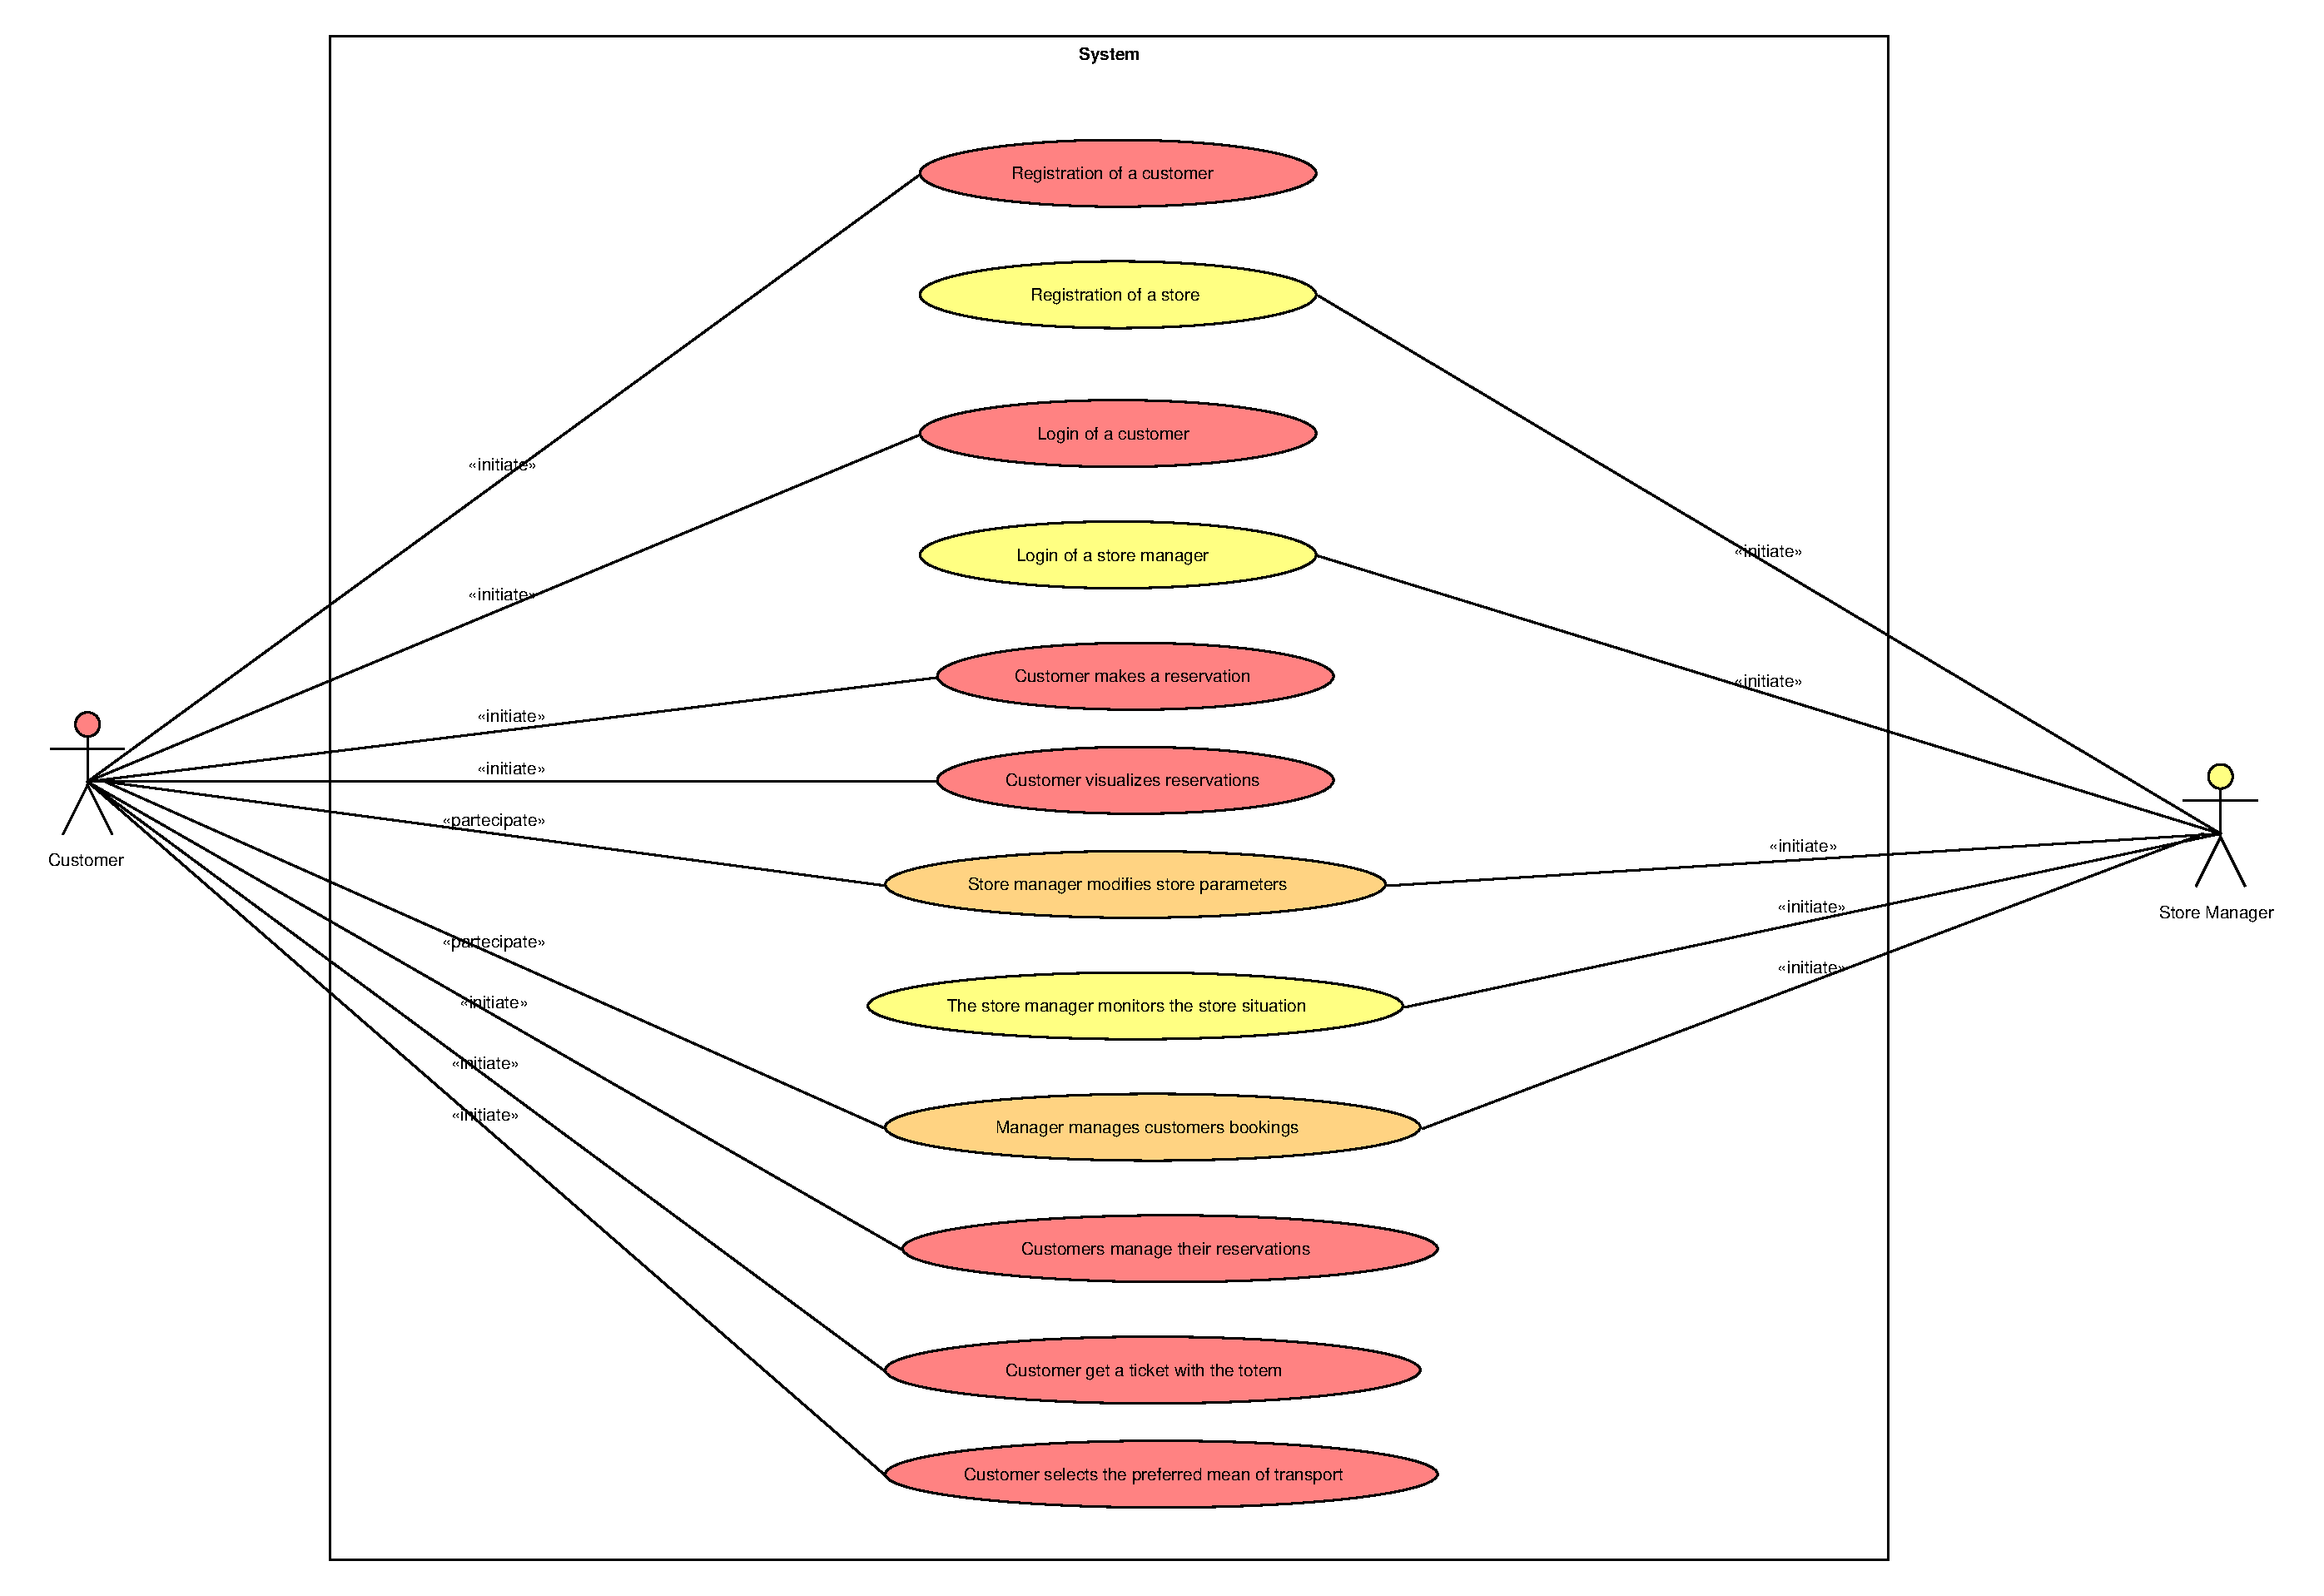
\includegraphics[scale=0.42]{UC/1_useCaseDiagram.pdf}\\
				\caption{\emph{Use Case Diagram}}
			\end{adjustwidth}
			
		\end{figure}
		\newpage
	\subsection{Performance Requirements}
	\emph{CLup} app is aimed to reduce gatherings due to the \emph{Covid-19} pandemic. So, some components needs a certain responsiveness. Here there are described some parts of the system that are critical to the scope of entire system
	\begin{itemize}
		\item {\bfseries Requests saving system:} when a client got a reservation, the system needs to process and save it in a very low time, less than 5 seconds, since the requests are fundamental in making estimations about waiting times.
		\item {\bfseries \emph{QR Code} processing:} each customer must scan his \emph{QR Code} when he enters the store. This means that, to avoid delays and crowds of people, the component processing \emph{QR Codes} must be really fast, and process them in no more than 5 seconds after the code is retrieved from the optical scanner.
		\item {\bfseries Ticket calling system:} as for \emph{QR Codes} processing, after a customer exits the store, the system must be able to process the next ticket to be called, if any, in a strict time, to avoid that people waits outside the store for long times. This process must not last more than 10 seconds.
		\item {\bfseries User notifier:} the system must responsively notify users that they must depart for the store in time, with a security margin to avoid lost of turns. 
		\item{\bfseries Application data updates:} when the customer need to use the application for any purpose, the app must be responsive, and each object required over the network must be available in no more than 5 seconds from its request; if the retrieve from the net fails, the app will show the local stored data to avoid embarrassing situations  (eg. the client must retrieve his \emph{QR Code} to access the store and internet isn't available) 
		\item{\bfseries Totem ticket printing: } the totem must process each request and print the ticket in no more than 5 seconds.
	\end{itemize} 
The above reported performance constraints must be always verified; that implies the system must be highly scalable to respect these timings. There isn't any limit on the number of registered stores and users, so the system must respect these constraints with at least 200 simultaneously connected users per each store inside the system.

	\newpage
	
	\subsection{Design Costraints}
		\subsubsection{Standards Compliance}
	System is compliant to some standards, such as:
	\begin{itemize}
		\item Generated \emph{QR Codes} are compliant to ISO/IEC 18004:2015 standard
		\item Network messages are exchanged through the internet protocol TCP/IP
	\end{itemize}
The same doesn't applies to requests of travel times and for mail sending, since they are achieved by \emph{APIs} of some external services.
		\subsubsection{Hardware Limitations}
		To work properly, \emph{CLup} needs some type of hardware, in base of the considered component.
		\begin{itemize}
			\item {\bfseries Customer Device:} Customer needs to have a device with a working network module, a \emph{GPS} module and a high resolution display for the QR-Cod scanners.
			\item {\bfseries Totem:} the totem must have a working network module, a ticket printer and a module to make possible interfacing between customer and totem.
			\item {\bfseries \emph{QR Code} readers:} \emph{QR Code} readers must have a working network module, and a optical scanner that takes no more than 5 seconds to read and interpret a \emph{QR Code} and its content.
		\end{itemize}
	
	\subsection{Software System Attributes}
		\subsubsection{Reliability}
		The system must have a  very low probability of failure (less than 0,0001\%) to avoid inconveniences in crowd managing.
		\subsubsection{Availability}
		Due to the critic aspects the application handles, is required a 99,99\% of system reliability. It means that the application will be down only for 52.60 minutes per year, an estimate that is acceptable. Having a greater downtime per year, may lead to inconveniences in handling the queue outside a store, bringing to a possible assembly of people.
		\subsubsection{Security}
		Each communication between client and server is made over a secure transport protocol (eg. TLS). For each request the system will authenticate the user so that everyone access only to data he is authorized. An encryption and decryption system must be implemented so that QRs' Content is encrypted to avoid someone can forge a malicious ticket. Moreover, each user password is stored using its hash value. 
		\subsubsection{Maintainability}
		Since rules can change in every moment, the software must be developed in an extendible way, so that it's easy to add new functions required by new restrictions. Moreover, the software can be used even if after the pandemic. So, it might be required to implement new feature to make the system more appealing.
		\subsubsection{Portability}
		The application must be portable on the majority mobile OSes. For this reasons, the app will use a notification service accessible through the OS APIs. Furthermore, the software is thought so that is possible to implement different external services in different versions.
		\subsection{Additional Specifications}
	The system guarantees unicity of each customer's email and of each store manager's ID.
	
	\newpage
	
\section{Formal Analysis Using Alloy}
	In this section a formal analysis of the previously described system is done, through the MIT's Alloy Tool.\\
	This analysis doesn't aim to cover all the system aspect. For example, no dynamic analysis have been done. Instead, here is conducted a static analysis of the most critic part the system: the absence of overcrowding in stores, and the fairness in reservations management.\\
	In particular, the principal functionalities that have been tested are:
	\begin{itemize}
		\item In each store department, there aren't more people than its capacity, and the maximum booked customers parameter is respected
		\item There isn't any customer with more than one spot on a store queue
		\item Reservations status is coherent with the list of reservations each store have
		\item No reservations on closure day, no same reservations across different store
		\item Coherence between timestamps of reservations notification, calling, entering and exit
		\item Customers are always notified to depart in time for the store through notification
	\end{itemize}
	\lstinputlisting[language=alloy]{AlloyModel/World.als}
	
	\begin{figure}[H]
		\begin{adjustwidth} {-3cm}{}
			\centering			
			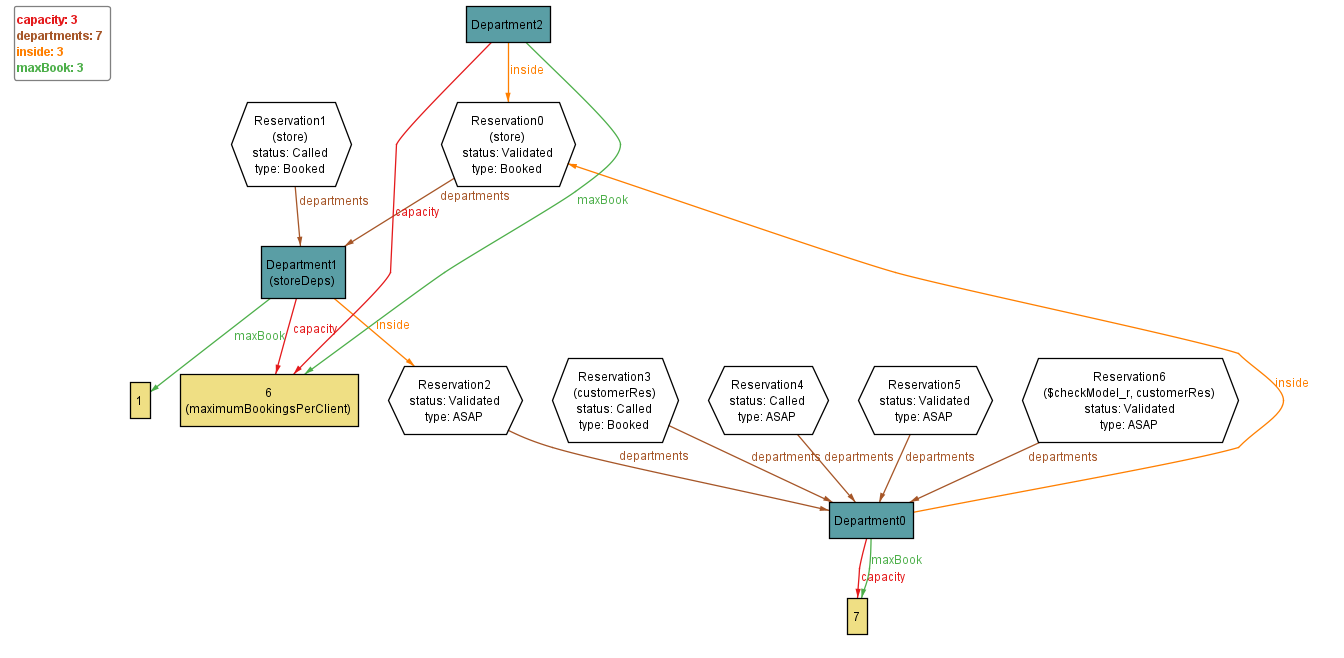
\includegraphics[scale=0.5]{AlloyModel/capacityRespected.png}\\
		\end{adjustwidth}
		\caption{\emph{Department Capacity respected. In this model, it's shown that the parameters of capacity and maximum allowed booked customers are respected}}
	\end{figure}
	
	
	\begin{figure}[H]
		\begin{adjustwidth} {-3cm}{}
			\centering
			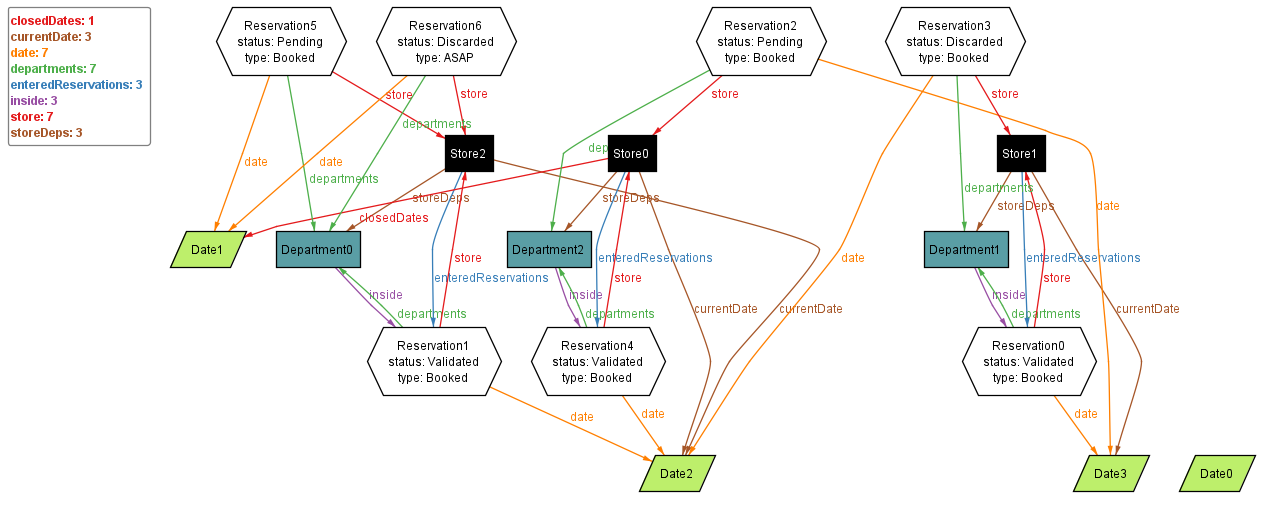
\includegraphics[scale=0.5]{AlloyModel/reservationStatus.png}\\	
		\end{adjustwidth}
		\caption{\emph{Coherent reservations status. Here the intent is to show that the status of all the reservations is coherent}}
	\end{figure}
	
	\begin{figure}[H]
		\begin{adjustwidth} {-3cm}{}
			\centering
			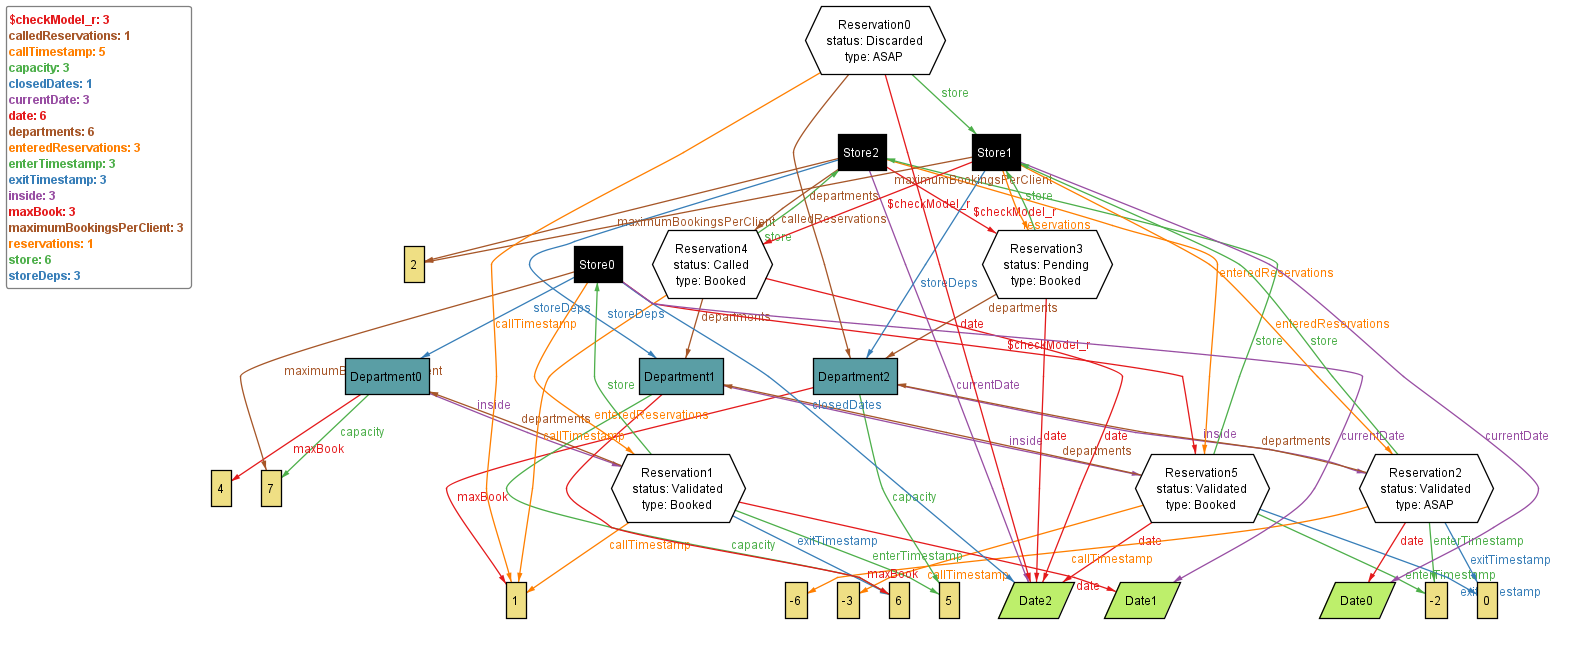
\includegraphics[scale=0.4, angle = 90]{AlloyModel/customerReservation.png}\\
		\end{adjustwidth}
		\caption{\emph{Customer reservations. Here is shown how constraints on customer's ability to make a reservation are respected}}
	\end{figure}

\section{References}
	\begin{itemize}
		\item Alloy Documentation: \url{https://alloytools.org/documentation.html}
		\item \LaTeX Documentation: \url{https://www.latex-project.org/help/documentation/}
	\end{itemize}	
	\bigskip
	
\section{Effort Spent}
	
	\bigskip
	\bigskip
	
	\begin{center}
		
		\renewcommand{\arraystretch}{1.2}
		
			\begin{tabular}[H]{|m{14em}|>{\centering\arraybackslash}m{12em}|}
				\rowcolor{gray!20}
				\hline
				\xrowht{5pt}
				\centering Task & Daniele Mammone's Hours \\
				\hline
				Introduction & 2 \\
				\hline
				Product Perspective & 2 \\
				\hline
				Product Functions & 6 \\
				\hline
				Domain Assumptions & 3 \\
				\hline
				State Charts & 4 \\
				\hline
				Use Cases & 8 \\
				\hline
				Class Diagram & 1 \\
				\hline
				External Interface Requirements & 1 \\
				\hline
				Mockups & 0 \\
				\hline
				Functional Requirements & 6 \\
				\hline
				Non-Functional Requirements & 1 \\
				\hline
				Formal Analysis Using Alloy & 6 \\
				\hline
				Scenarios & 1\\
				\hline
				Revision & 5\\
				\hline
				Document Drafting & 3 \\
				\hline
				Total Hours & 49\\
				\hline
			\end{tabular}
		
	\end{center}

	\bigskip
	\bigskip
	\bigskip
	\bigskip

	\begin{center}
		
		\renewcommand{\arraystretch}{1.2}
		
		\begin{tabular}[h!]{|m{14em}|>{\centering\arraybackslash}m{12em}|}
			\rowcolor{gray!20}
			\hline
			\xrowht{5pt}
			\centering Task & Gianmarco Naro's Hours\\
			\hline
			Introduction & 2 \\
			\hline
			Product Perspective & 3 \\
			\hline
			Product Functions & 3 \\
			\hline
			Domain Assumptions & 3 \\
			\hline
			State Charts & 1 \\
			\hline
			Use Cases & 4 \\
			\hline
			Class Diagram & 3 \\
			\hline
			External Interface Requirements & 1 \\
			\hline
			Mockups & 0 \\
			\hline
			Functional Requirements & 7 \\
			\hline
			Non-Functional Requirements & 1 \\
			\hline
			Formal Analysis Using Alloy & 2 \\
			\hline
			Scenarios & 2\\
			\hline
			Revision & 5\\
			\hline
			Document Drafting & 6 \\
			\hline
			Total Hours & 43\\
			\hline
		\end{tabular}
	\end{center}

	\bigskip

	\begin{center}
		
		\renewcommand{\arraystretch}{1.2}
		
		\begin{tabular}[h!]{|m{14em}|>{\centering\arraybackslash}m{12em}|}
			\rowcolor{gray!20}
			\hline
			\xrowht{5pt}
			\centering Task & Massimo Parisi's Hours \\
			\hline
			Introduction & 2 \\
			\hline
			Product Perspective & 2 \\
			\hline
			Product Functions & 2 \\
			\hline
			Domain Assumptions & 3 \\
			\hline
			State Charts & 2 \\
			\hline
			Use Cases & 7 \\
			\hline
			Class Diagram & 3 \\
			\hline
			External Interface Requirements & 4 \\
			\hline
			Mockups & 5 \\
			\hline
			Functional Requirements & 5 \\
			\hline
			Non-Functional Requirements & 1 \\
			\hline
			Formal Analysis Using Alloy & 2 \\
			\hline
			Scenarios & 0\\
			\hline
			Revision & 2\\
			\hline
			Document Drafting & 2 \\
			\hline
			Total Hours & 42\\
			\hline
		\end{tabular}
	\end{center}
	
\end{document}